%
% -------------------------------------------------------------------
% Electrodynamics lecture at TU Berlin, read by Prof. Holger Stark
% -------------------------------------------------------------------
%
%
% Anmerkungen: 

% - Sections
% Der Stil der sections und deren Nummerierungen orientiert sich an der Vorlesung. 
% Statt subsection*{} gibt es einen neuen Befehl subsectiona{}, der die Unter-
% überschriften nicht nummeriert, aber trotzdem in das Inhaltsverzeichnis integriert. 

% - Vektorpfeile
% Die Vektorpfeile des esvect-Pakets bieten ein besseres Spacing, vorallem wenn
% danach eine geschlossene Klammer oder eine Hochstellung folgt. In der Datei 
% esvectmod.sty in diesem Projekt ist noch eine kleine Verbesserung des Layouts drin, 
% aber ganz perfekt funktionieren Vektorpfeile in Latex nie. Weiter unten gibt es noch 
% eine Option, alle Vektoren stattdessen fettgedruckt darzustellen...

% - Abbildungen
% Alle Abbildungen sind vektorbasierte Skizzen im PDF-Format. Das Paket wrapfig erlaubt
% zwar Abbildungen in den Textfluss zu integrieren, aber manchmal ist der Abstand
% unter der Abbildung zum Text zu groß/klein. Dann kann mit \vspace{10mm} der Abstand
% vergrößert oder mit negativen Werten verkleinert werden. 

\documentclass[hidelinks, 11pt]{scrbook} 

\usepackage[left=2cm, right=2cm, bottom=1.5cm, top=1.5cm, includeheadfoot]{geometry} 
\usepackage[T1]{fontenc} 
\usepackage[utf8]{inputenc} 
\usepackage{graphicx} 
\usepackage{multirow} 
\usepackage{tabularx} 
\usepackage{xcolor} 
\usepackage{amsmath} 
\usepackage{amssymb} 
\usepackage{amsfonts} 
\usepackage{amsxtra} 
\usepackage{mathtools} 
\usepackage{upgreek} 
\usepackage{enumerate} 
\usepackage{tensor} 
\usepackage{float}
\usepackage[english,ngerman]{babel}
\usepackage{siunitx}
\usepackage{longtable}
\usepackage{cancel}
\usepackage{wrapfig}

\usepackage{lmodern}
\usepackage[f]{esvectmod}
\usepackage[font=footnotesize]{caption}
\sisetup{locale = DE, separate-uncertainty}  
\usepackage[immediate]{silence}
\WarningFilter[temp]{latex}{Command} % filter underline/underbar command warning from sectsty 

% --------------------------
% spacing

\setlength{\parindent}{0em}
\setlength{\parskip}{1em}

\usepackage[hang]{footmisc}
\setlength{\footnotemargin}{3mm} % space between number and content of footnote
\setlength{\skip\footins}{.5cm} % space between body and footnote section
\setlength{\footnotesep}{0.5cm}  % space between footnotes

%\renewcommand{\arraystretch}{1}

\raggedbottom

\makeatletter
\renewcommand\@pnumwidth{2em} % fix toc overfull hbox
\makeatother

% --------------------------
% section styles

%\usepackage{sectsty}
%\renewcommand{\thesection}{\Alph{section}} 
%\newcommand{\subsubsectiona}[1]{\subsubsection*{#1}}%\addcontentsline{toc}{subsection}{#1}} 
%\subsubsectionfont{\normalfont\large\underline}
\newcommand{\example}[1]{\paragraph{#1:}}

\makeatletter
\renewcommand\subsubsection{\@startsection{subsubsection}{3}{\z@}%
                                     {-3.25ex\@plus -1ex \@minus -.2ex}%
                                     {1.5ex \@plus .2ex}%
                                     {\normalfont\normalsize}}
\makeatother
\newcommand{\subsubsectiona}[1]{\subsubsection*{\underline{#1}}}
                                   
%\labelformat{section}{\thechapter#1} % section refs should include chapter letter

% --------------------------
% math
\DeclareMathOperator{\grad}{grad} 
\DeclareMathOperator{\divg}{div} 
\DeclareMathOperator{\rot}{rot} 

\newcommand{\upupharpoons}{\upharpoonleft\!\upharpoonright}
\newcommand{\updownharpoons}{\upharpoonleft\!\downharpoonright}
% pm sign with minus in paretheses
\newcommand\varpm{\mathbin{\vcenter{\hbox{
  \oalign{\hfil$\scriptstyle+$\hfil\cr\noalign{\kern-.3ex}$\scriptscriptstyle({-})$\cr}
}}}}
% mp sign with plus in parentheses
\newcommand\varmp{\mathbin{\vcenter{\hbox{
  \oalign{$\scriptstyle({+})$\cr\noalign{\kern-.3ex}\hfil$\scriptscriptstyle-$\hfil\cr}
}}}}
% vector than can be primed without looking ugly af 
%\newcommand*\pvec[1]{\vec{#1}\mkern2mu\vphantom{#1}} 
%\renewcommand{\pvec}[1]{\vec{#1}} 
% differential operator have a non-italic d in German equation typesetting 
%\newcommand*\diff{\mathop{}\!\diff } 
\newcommand{\diff}{\text{d}}	 
\newcommand{\Angstroem}{\text{\normalfont\AA}}   
\newcommand{\Abbref}[1]{Abb.~\ref{#1}} 
% vector arrow that does not clash with exponents 
\makeatletter 
\newcommand{\svec}[1]{\vec{#1}\@ifnextchar{^}{\,}{}} 
\makeatother 
% NO, better use esvect, much better spacing 
%\let\oldvec\vec 
%\renewcommand{\vec}[1]{\oldvec{\mkern2mu#1\mkern2mu}} 
%\renewcommand{\vec}[1]{\oldvec{#1\mkern-2mu}} 
%\renewcommand{\vec}[1]{\vv{#1}} % esvect vector 
% Alternative: bold non-cursive symbols for vectors instead of arrows 
\renewcommand{\vec}[1]{\mathbf{#1}} 
%\renewcommand{\svec}[1]{\vec{#1}} 

\newcommand\equivalence{\;\Leftrightarrow\;}
\newcommand\implication{\;\Rightarrow\;}

% Alternative: bold non-cursive symbols for vectors instead of arrows
%\renewcommand{\vec}[1]{\mathbf{#1}}

% set figure description
\addto\captionsngerman{
  \renewcommand{\figurename}{Abb.}
  \renewcommand{\tablename}{Tab.}
}
\graphicspath{{images/}} 
\usepackage[strict]{changepage}

% for formal definitions
\usepackage{framed}

% environment derived from framed.sty: see leftbar environment definition
\definecolor{formalbar}{rgb}{0.1,0.1,.2}
\definecolor{formalshade}{rgb}{0.95,0.95,1}

% Quote box for important statements
\newenvironment{formal}{%
  \def\FrameCommand{%
    \hspace{1pt}%
    {\color{formalbar}\vrule width 2pt}%
    {\color{formalshade}\vrule width 4pt}%
    \colorbox{formalshade}%
  }%
  \MakeFramed{\advance\hsize-\width\FrameRestore}%
  \noindent\hspace{-4.55pt}% disable indenting first paragraph
  \begin{adjustwidth}{}{7pt}%
  \vspace{-10pt}\vspace{2pt}%
}
{%
  \vspace{2pt}\end{adjustwidth}\endMakeFramed%
}

% !TEX root = Theo_III.tex

\usepackage{tikz}
\usetikzlibrary{arrows.meta,positioning,decorations.markings,intersections,calc,decorations.pathreplacing,external}
%\tikzexternalize[prefix=figures/] % activate

\tikzset{
    object color/.style={blue!40!black!80!white},
    object style/.style={object color,thick},
    legreen/.style={green!50!black},
    lorange/.style={red!60!yellow!70!black!90!white},
    polarisation color/.style={purple},
    charge color/.style={blue!50!white!70!black},
    red laser/.style={red!70!black},
    moving system color/.style={blue!60!black!70!white},
    coordsystem/.style={very thin, color=#1!50},
    invisible point/.style={circle,inner sep=0pt,outer sep=0pt,minimum size=0pt},
    point/.style={invisible point,fill=black,minimum size=4pt},
    arr/.style={->,>={Stealth},thin},
    rarr/.style={<-,>={Stealth},thin},
    midarrow/.style={postaction=decorate,decoration={markings, mark=at position #1 with {\arrow{Stealth}}} },
    midarrow/.default=.5,
    rmidarrow/.style={postaction=decorate,decoration={markings, mark=at position #1 with {\arrowreversed{Stealth}}} },
    rmidarrow/.default=.5,
    distance marker/.style={|<->|,>={Stealth}},
}
\tikzstyle{every node}=[font=\footnotesize]


\newcommand{\tfigTitel}{
    \begin{tikzpicture}
        \pgfmathsetmacro{\shadowangle}{132}
        \newlength{\shadowdistance}
        \pgfmathsetlength{\shadowdistance}{0.1ex}
        \pgfmathsetmacro{\shadowopacity}{1}
        \pgfmathsetmacro{\shadowspread}{0.003}
        \pgfmathsetmacro{\shadowsize}{5}
        \pgfmathtruncatemacro{\totshadow}{100}
        \path[red laser,opacity={\shadowopacity/\totshadow},shift={({132-180}:\shadowdistance)},scale={1+\shadowsize}] 
        foreach \nshadow [evaluate=\nshadow as \angshadow using \nshadow/\totshadow*360] in {1,...,\totshadow}{
            node[align=center] at (\angshadow:\shadowspread) {\huge Theoretische Physik 3\\ \\ \\
            \Large Elektrodynamik}
            };
        \node[align=center] at (0,0) {\huge Theoretische Physik 3\\ \\ \\ \Large Elektrodynamik};
    \end{tikzpicture}
}

\newcommand{\tfigVolumeWithNormal}{
    \begin{tikzpicture}[scale=2]
        \draw[object style] (0,1,1) -- (0,1,0) -- (1,1,0) -- (1,0,0)
        -- (1,0,1) -- (0,0,1) --(0,1,1) -- (1,1,1) 
        -- (1,0,1) --  (1,1,1) -- (1,1,0);
        % \node at (.5,.5,1) {$\vec a(\vec r)$};
        \node at (.5,.5,1) {$V$};
        \draw[arr] (1,.5,.5) -- +(0.5,0,0) node[right] {$\hat{\vec n}$};
    \end{tikzpicture}
}

\newcommand{\tfigAreaWithCurveAndNormal}{
    \begin{tikzpicture}[scale=2.3]
        \draw[object style,rmidarrow=.1] (0,0) rectangle (1,1) node[below,right] {$C$};
        \node at (.5,.5) {$F$};
        \node[point, label={$\hat{\vec n}$}] at (-.2,.6) {};
        \draw[decorate, decoration = {brace, mirror}]  (0,-.1) -- +(1,0) node[midway, below,yshift=-3pt] {$\Delta r_C$};
        \draw[arr] (1.15, .4) -- +(0,.3) node[midway, right] {$\hat{\vec t}_C$};
    \end{tikzpicture}
}

\newcommand{\tfigLinienintegral}{
    \begin{tikzpicture}[scale=2, clr/.style={lorange}]
        \coordinate (A) at (0,0);
        \coordinate (NC) at (0,.2);
        \coordinate (B) at (1.3,2);
        \coordinate (FC) at (.5,.1);
        \coordinate (C2) at (1.5,1);
        \coordinate (R) at (0.65,1);
        
        \node[point, label=right:{$\vec r_0$}] at (A) {};
        \node[point, label=right:{$\vec r_1$}] at (B) {};
        
        \draw[object style] (A) .. controls ($(A)+(NC)$) and ($(R)-(FC)$) .. (R) .. controls  ($(R)+(FC)$) and ($(B)-(NC)$) .. (B)
          node[very near end, left] {$C$};
        
        \node[point,clr,label={below,clr}:{$\vec r$}] at (R) {};
        \draw[arr,clr] (R) -- ($(R)+(FC)$) node[below] {$\diff \vec r$};
        \draw[arr, legreen] (-.1,.2) -- (-.01,.5) node[midway, left] {$s$};
    \end{tikzpicture}
}

\newcommand{\tfigHalbkugel}{
    \begin{tikzpicture}[scale=2]
        \coordinate (A) at (0,0);
        \draw[object style] (0,0) arc (0:180:1) node[midway, above] {$F$};
        \draw[object style,dashed] (0,0) arc (0:180:1 and .3);
        \draw[object style,rmidarrow] (0,0) arc (0:-180:1 and .3) node[midway, below] {$C=\partial F$};
        
        \draw[arr] (-.4,.5) -- +(45:.5) node[right] {$\diff \vec f=\hat{\vec n}\diff f$};
    \end{tikzpicture}
}

\newcommand{\tfigCoulombPointCharges}{
    % Forces on to charges
    \begin{tikzpicture}[scale=1]
        \coordinate (O) at (0.0,0.0);
        \coordinate (Q1) at (1.0,1.1);
        \coordinate (Q2) at (2.0,.1);
        \coordinate (F1) at ($(Q1)+(Q1)-(Q2)$);
        \coordinate (F2) at ($(Q2)+(Q2)-(Q1)$);
        
        \node[point, charge color] (Q1 node) at (Q1) 
            [label={east, yshift=1mm, charge color}:$q_1$] {} 
            edge[arr] node[at end, above] {$\vec F_1$} (F1);
        \node[point, charge color] (Q2 node) at (Q2) 
            [label={east, yshift=1mm, charge color}:$q_2$] {} 
            edge[arr] node[at end, below] {$\vec F_2$} (F2)
            edge[arr] node[midway, right, yshift=1mm, xshift=1mm] {$\vec r_1-\vec r_2$} (Q1 node);
        \node[invisible point] at (O) {} 
        edge[arr] node[midway, below] {$\vec r_2$} (Q2 node)
        edge[arr] node[midway, anchor=south east] {$\vec r_1$} (Q1 node);
    \end{tikzpicture}
}

% äquipotentiallinien und elektrische feld Linien zweier ungleichnamiger ladungen
\newcommand{\tfigDipoleFieldPotential}{
    \begin{tikzpicture}[scale=1.3]
        \coordinate (Q1) at (-1,0);
        \coordinate (Q2) at (1,0);
        \coordinate (A1) at (-2,0);
        \coordinate (A2) at (2,0);
        \coordinate (T) at (0,1.6);
        \draw[midarrow] (Q1) .. controls +(45:.7) and +(135:.7) .. (Q2);
        \draw[midarrow] (Q1) .. controls +(75:1)  and +(105:1)  .. (Q2);
        \draw[midarrow] (Q1) .. controls +(105:1.7) and +(75:1.7) .. (Q2);
        \draw[midarrow] (Q1) .. controls +(135:.7) and +(-135:.7) .. ($(Q1)+(T)$);
        \draw[rmidarrow] (Q2) .. controls +(45:.7) and +(-45:.7) .. ($(Q2)+(T)$);
        
        \draw[dashed] 
            let \p1=(Q1),\p2=(Q2) in
            (0,0) -- (T)
            (\x1/3,0) .. controls +(90:1) and +(-50:.3) .. ($(T)+{3/4}*(Q1)$)
            (\x2/3,0) .. controls +(90:1) and +(-130:.3) .. ($(T)+{3/4}*(Q2)$)
            (\x1-\x1/3,0) arc(0:180:1/3)
            (\x2+\x2/3,0) arc(0:180:1/3);
        
        \node[point, charge color] (Q2 node) at (Q2) 
            [label=south:$-q$] {} ;
        \node at (A2) {} 
            edge[arr] node {} (Q2 node);
        \node[point, charge color] (Q1 node) at (Q1) 
            [label=south:$q$] {} 
            edge[arr] node {} (A1)
            edge[arr] (Q2 node);
    \end{tikzpicture}
}

\newcommand{\tfigEfieldAndPotLinesAndChargeDensitityHomoChargedSphere}{
    % Field and equipotential lines of a charged sphere
    \begin{tikzpicture}[
        scale=2,
        potential color/.style={violet!60!black}
    ]
    \coordinate (O) at (0.0,0.0);

    \foreach \angle in {0,45,...,325}
        \draw[arr] (O) -- (\angle:1);
    \foreach \radius in {0,0.2,...,0.8}
        \draw[dashed,potential color] (O) circle [radius=\radius];
        
    \node[potential color] at (-20:1) {$V_r$};
    \node at (-150:1.2) {$\vec E$};

    \draw[charge color] (O) circle [radius=.7];
    \draw[arr, charge color] (O) -- (60:0.7) node[near end, left] {$R$};

    \begin{scope}[shift={(2.3,-.6)}]
        \coordinate (A) at (1.2, 0.8);
        
        \draw[arr] (0,0) -- (0, 1.3) 
            node[at end, anchor=south east] {$\rho(r)$};
        \draw[arr] (0,0) -- (1.6, 0) 
            node[at end, anchor=north west] {$r$};
        \draw[charge color] let \p1 = (A) in
            (0, \y1) -- (A) 
            node[at start, left] {$\rho_0$}
            -- (\x1, 0)
            node[charge color, below] {$R$};
    \end{scope}
    \end{tikzpicture}
}
\newcommand{\tfigEfieldAndPotentialHomoChargedSphere}{
    % field and potential function for sphere
    \begin{tikzpicture}[scale=3]
        \coordinate (A) at (0.8, 0.8);
        
        % electric field
        \draw[arr] (0,0) -- +(0, 1.1) 
            node[at end, anchor=south east] {$E(r)$};
        \draw[arr] (0,0) -- +(1.8, 0) 
            node[at end, anchor=north west] {$r$};
            
        \draw[charge color,yscale=.2] 
            let \n1={0.5},\n2={1.7} in
            plot[domain=0:\n1] (\x,\x/\n1^3) 
            node[above left] at (\n1/2,\n1/2/\n1^3) {$\propto r$} 
            plot[domain=\n1:\n2] (\x,1/\x^2) 
            let \n4={.5*\n2-.5*\n1+\n1} in % x value of middle point of second graph 
            node[above] at (\n4,1/\n4^2) {$\displaystyle\propto\frac{1}{r^2}$};
        \draw[dashed, very thin] (0.5,.8) -- +(0,-.8) 
            node[below] {$R$};
            
        % potential
        \begin{scope}[shift={(2.5,0)}]
            \draw[arr] (0,0) -- +(0, 1.1) 
                node[at end, anchor=south east] {$\phi(r)$};
            \draw[arr] (0,0) -- +(1.8, 0) 
                node[at end, anchor=north west] {$r$};
            \draw[charge color,yscale=.3] 
                let \n1={0.5},\n2={1.7} in 
                plot[domain=0:\n1] (\x,3/\n1/2 -\x^2/\n1^3/2)
                node[right, xshift=-25,yshift=25] {$\displaystyle\propto \frac3{2R}-\frac{r^2}{2R^3}$}
                plot[domain=\n1:\n2] (\x,1/\x)
                let \n4={.5*\n2-.5*\n1+\n1} in % x value of middle point of second graph 
                node[above] at (\n4,1/\n4) {$\displaystyle\propto\frac{1}{r}$};
                
            \draw[dashed, very thin] (0.5,1/1.7) -- +(0,-1/1.7) 
                node[below] {$R$};
        \end{scope}
    \end{tikzpicture}
}

\newcommand{\tfigThreeConductors}{
    % Anordnung von elektrischen Leitern Li mit Ladungen Qi und Potentialen φi.
    \begin{tikzpicture}[clr/.style={legreen},scale=1.2]
        \draw[rotate=45] 
            (0,0) ellipse [x radius=1.2, y radius=.5] 
            node {$L_1$} node[charge color] at +(-.9,0) {$Q_1$}
            node[clr] at +(.2,.8) {$\phi_1$} ;
        \draw[rotate=0] 
            (2,-2) ellipse [x radius=.5, y radius=.55] 
            node {$L_2$} node[charge color] at +(-.5,-.6) {$Q_2$}
            node[clr] at +(.2,.8) {$\phi_2$};
        \draw[rotate=3] 
            (4,0) ellipse [x radius=.8, y radius=.4] 
            node {$L_3$} node[charge color] at +(-.5,-.6) {$Q_3$}
            node[clr] at +(.3,.6) {$\phi_3$};
        \node at (5,-1.4) {$\ldots$};
    \end{tikzpicture}
}

\newcommand{\tfigSpecialCapacitors}{

% capacitors
\begin{tikzpicture}[scale=1.2]
    \begin{scope}
        \coordinate (A0) at (-.7,0);
        \coordinate (A1) at (-.7,2.5);
        \coordinate (B0) at (.7,0);
        \coordinate (B1) at (.7,2.5);
        \draw[very thick] (A0) -- (A1) 
        node[at start,below,legreen] {$\phi_1$}
        node[at end,above] {$-Q$};
        \draw[very thick] (B0) -- (B1) 
        node[at start,below,legreen] {$\phi_2$}
        node[at end,above] {$Q$};
        
        \draw[distance marker] ($(A0)!.5!(A1)$) -- ($(B0)!.5!(B1)$) node[midway,below] {$d$};
    \end{scope}
    
    \begin{scope}[shift={(3.2cm,1.2cm)}]
        \coordinate (O) at (0,0);
        \draw[thick] (O) circle[radius=.6];
        \draw[thick] (O) circle[radius=1];
        
        \draw[arr] (O) -- (30:1) node[pos=.9, below,yshift=-3] {$r_2$};
        \draw[arr] (O) -- (45:.6) node[midway, above, left,yshift=3] {$r_1$};
        \node[legreen] at (-160:1.2) {$\phi_2$};
        \node[legreen] at (-140:.4) {$\phi_1$};
        
        \draw (135:1) -- +(45:1) (-45:1) -- +(45:1);
        \begin{scope}
            \clip (O) circle[radius=1];
            \draw (135:.6) -- +(45:1) (-45:.6) -- +(45:1);
        \end{scope}
    \end{scope}
    
    \begin{scope}[shift={(7cm,1.2cm)}]
        \coordinate (O) at (0,0);
        \draw[thick] (O) circle[radius=.6];
        \draw[thick] (O) circle[radius=1];
        
        \draw[arr] (O) -- (30:1) node[pos=.9, below,yshift=-3] {$r_2$};
        \draw[arr] (O) -- (45:.6) node[midway, above, left,yshift=3] {$r_1$};
        \node[legreen] at (-160:1.2) {$\phi_2$};
        \node[legreen] at (-140:.4) {$\phi_1$};
    \end{scope}
\end{tikzpicture}

}

\newcommand{\tfigComplexProblemsConformalMap}{
    \begin{tikzpicture}
        \draw (-3,0) circle [radius=1];
        \node[align=center] at(-5,0) {Lösung $\phi$\\bekannt};
        \draw[arr] (-1,0) .. controls +(20:.7) and +(160:.7) .. (1,0) node[align=center,midway,above,yshift=.2cm] {Konforme\\Abbildung}
        node[align=center,midway,below,yshift=-.4cm] {$\begin{aligned}
            z&\rightarrow w=w(z) \\
            f(z)&\rightarrow f(z(w))=g(w)
        \end{aligned}$};
        
        \begin{scope}[shift={(4.5,.2)}]
        \coordinate (A) at (-2,-1);
        \coordinate (B) at (-1.8,-.8);
        \coordinate (C) at (-1.8,.-.2);
        \coordinate (D) at (-1.8,.3);
        \coordinate (E) at (-1.3,.5);
        \coordinate (F) at (-0.8,.3);
        \coordinate (G) at (-0.2,.4);
        \coordinate (H) at (0.8,.6);
        \coordinate (I) at (0.8,-1);
        \coordinate (J) at (-1.1,-1.4);
        
        \node[align=center] at(2.8,0) {$\mathfrak{R}(g(w)$ löst \\$\nabla^2\mathfrak{R}(g(w)=0$};
        
        \draw (A) 
        .. controls +(-150:.1) .. (B) 
        .. controls +(30:.1) and +( -50: 1.1) ..(C) 
        .. controls +(130: 1.1) and +(140:1) .. (D)
        .. controls +(-40:.5) and +(-100:.4) .. (E) 
        .. controls +(80:.5) and +(120:.8) .. (F) 
        .. controls +(-60:.8) and +(-95:1) .. (G)
        .. controls +(85:.8) and +(120:1) .. (H)
        .. controls +(-60:1.5) and +(5:.9) .. (I)
        .. controls +(-175:.7) and +(10:.4) .. (J)
        .. controls +(-170:.7) and +(10:.4) .. cycle;
        \end{scope}
    \end{tikzpicture}
}

\newcommand{\tfigWatermolecule}{

    % water molecule
    \begin{tikzpicture}[scale=3]
        \node[circle] (H1) at ($(-90+104.45/2:1)$) {$\mathrm{H}^+$};
        \node[circle] (H2) at ($(-90-104.45/2:1)$) {$\mathrm{H}^+$};
        \node[circle] (p) at (-90:.8) {};
        \node[circle] at (0,0) [label={east,xshift=-2mm,yshift=1mm}:-] {O} 
            edge (H1) 
            edge (H2) 
            edge[arr, charge color] 
            node[midway, left] {$\vec p$} (p);
    \end{tikzpicture}
}

\newcommand{\tfigElementalQuadrupoles}{
    % elemental quadrupoles
    \begin{tikzpicture}[
        scale=1.2,
        charge/.style={point, charge color, outer sep=2mm}
    ]
    \node[charge] (Q1) at (-1,-1) [label={left}:$+q$] {};
    \node[charge] at (-1,1) [label={left}:$-q$] {} edge[arr] (Q1);
    \node[charge] (Q2) at (1,1) [label={left}:$+q$] {};
    \node[charge] at (1,-1) [label={left}:$-q$] {} edge[arr] (Q2);


    \begin{scope}[shift={(5,0)}]
        \node[charge] (Q3) at (0,1) [label={left}:$+q$] {};
        \node[charge] (Q4) at (0,-1) [label={left}:$+q$] {};
        \node[charge, inner sep=1mm] at (0,0) [label={left}:$-2q$] {} 
            edge[arr] (Q3) 
            edge[arr] (Q4);
    \end{scope}
    \end{tikzpicture}
}


\newcommand{\tfigDipoles}{
    % dipoles
    \begin{tikzpicture}[scale=1]
        \begin{scope}[shift={(-1cm,0)}]
            \coordinate (A0) at (0,0);
            \coordinate (A1) at (-1,1.2);
            \coordinate (B0) at (1,-.2);
            \coordinate (B1) at (1.3,1.4);
            
            \draw[arr] (A0) -- (A1) node[midway, anchor=north east] {$\vec p_1$};
            \draw[arr] (B0) -- (B1) node[midway, right] {$\vec p_2$};
            \draw[arr] ($(A0)!.5!(A1)$) -- ($(B0)!.5!(B1)$) node[midway, above] {$\vec r$};
        \end{scope}
        \begin{scope}[shift={(3.5cm,0)}]
            \draw[arr] (0,0) -- +(0,0.5);
            \draw[arr] (0,0.6) -- +(0,0.5);
            \node at (0,-.5) {$U$ minimal};
        \end{scope}
        \begin{scope}[shift={(7cm,0)}]
            \draw[arr] (-.8,0.55-0.25) -- +(0,0.5);
            \draw[arr] (-.4,0.55-0.25) -- +(0,0.5);
            \draw[rarr] (.8,0) -- +(0,0.5);
            \draw[arr] (.8,0.6) -- +(0,0.5);
            \node at (0,-.5) {$U$ maximal};
        \end{scope}
        \begin{scope}[shift={(11cm,0)}]
            \draw[arr] (-.2,0.55-0.25) -- +(0,0.5);
            \draw[rarr] (.2,0.55-0.25) -- +(0,0.5);
            \node at (0,-.5) {Lokales Minimum};
        \end{scope}
    \end{tikzpicture}
}

\newcommand{\tFigRandbedingungenDielektrikum}{
    \begin{tikzpicture}[scale=1]
    \draw
    (0,0) .. controls (1.8,.6) and +(-3,.4) .. (7,.3)
    node[pos=.9, above, sloped] {$\vec E^{(2)},\vec D^{(2)},\vec P^{(2)}$}
    node[pos=.9, below, sloped] {$\vec E^{(1)},\vec D^{(1)},\vec P^{(1)}$}
    node[very near start, above, sloped] {$\varepsilon_2$}
    node[very near start, below, sloped] {$\varepsilon_1$}
    node[pos=.65,below,sloped] {$\sigma(\vec r)$};

    \coordinate (P) at (2, .446);

    \node[point] at (P) {};
    \draw[arr]
    (P) -- +(7:1)
    node[midway, below] {$\hat{\vec t}$};
    \draw[arr]
    (P) -- +(97:1)
    node[midway, left] {$\hat{\vec n}$};
    \end{tikzpicture}
}


\newcommand{\tfigDielektrischeBrechung}{
    \begin{tikzpicture}[
        scale=2,
        incolor/.style = {red!50!black},
        outcolor/.style = {blue!50!black}
    ]
    \coordinate (Start) at (-140:1);
    \coordinate (StartFoot) at ($(Start) + (0,.2)$);
    \coordinate (Middle) at (0,0);
    \coordinate (End) at (70:0.7);
    \coordinate (EndFoot) at (0,0.2);

    \draw[arr,legreen] 
        (Start) -- (Middle) 
        node[at start,anchor=north west] {$\vec D^{(1)}$}
        (Middle) -- (End)
        node[at end,anchor=south west] {$\vec D^{(2)}$};
    \draw[arr] ($.6*(Start)$) -- (Middle) 
        node[at start,anchor=south east] {$\vec E^{(1)}$};
    \draw[arr] 
        (Middle) -- ($.7*(End)$)
        node[at end,anchor=north west] {$\vec E^{(2)}$};

    \draw[thick] (-1,0) -- +(2,0);
    \draw[dashed] (0,-1) -- +(0,2);
    \node at (-0.5,.7) {$\varepsilon_2<\varepsilon_1$};
    \node at (0.5,-.7) {$\varepsilon_1$};
    \end{tikzpicture}
}


\newcommand{\tfigMessungVonFeldDurchRandbedingungen}{
    \begin{tikzpicture}[probeladung/.style={point,outer sep=1mm}]
    \draw[yshift=-1mm] (-5,0) rectangle +(3,.2);
    \node (E0) at (-5.8,0) {$\vec E_0$} edge[arr] (-4.8,0);
    \node[probeladung] (P1) at (-2.8,0) {};
    \node at (-5+3/4,-.8) {$\varepsilon_r$};
    \foreach \x in {1,2,...,4}{
        \draw[arr, object color] (3/4*\x-5-3/8,1.3) -- +(0,-2.6);
    };

    \draw[xshift=-1mm] (3.5,1.4) rectangle +(.2,-2.8);
    \node (E0) at (5.8,0) {$\vec E_0$} edge[arr] (3.5,0.7);
    \node[probeladung] (P2) at (3.5,0) {};
    \node at (5-3/4,-.8) {$\varepsilon_r$};
    \foreach \x in {1,2,...,4}{
        \draw[arr, object color] (3/4*\x+2-3/8,1.3) -- +(0,-2.6);
    };
    \node[object color] at (-3.5,1.8) {$\vec E\parallel\vec D$};
    \node[object color] at (3.5,1.8) {$\vec E$};

    \node at (0,0) {Probeladung} edge[arr] (P1) edge[arr] (P2);
    \end{tikzpicture}
}

\newcommand{\tfigDielektrischeKugelHomogenesEFeld}{
    \begin{tikzpicture}[scale=1,earr/.style={arr,object color}]
    \draw[thick] (0,0) circle[radius=1];
    \draw[arr] (0,0) -- (45:1) node[midway, anchor=south east] {$R$};
    \node at (0,-.7) {$\varepsilon_r> 1$};
    \draw[earr] (-2.5,2) -- +(5,0);
    \draw[earr] (-2.5,-2) -- +(5,0);
    \draw[earr] (-2.5,0) -- (-1,0) (1,0) -- +(1.5,0);
    \foreach \i in {1,-1} {
        \draw[earr] (-2.5,\i*2/3) .. controls +(0:.7) and +(\i*160:.3) .. (\i*160:1) (\i*20:1) .. controls +(\i*20:.3) and +(\i*180:.7) .. (2.5,\i*2/3); 
        \draw[earr] (-2.5,\i*4/3) .. controls +(0:1) and +(180:.5) .. (0,\i*1.1) .. controls +(0:.5) and +(180:1) .. (2.5,\i*4/3);
    };

    \draw[earr] (160:1) -- (20:1);
    \draw[earr] (180:1) -- (0:1);
    \draw[earr] (-160:1) -- (-20:1);

    \draw[arr] (3,0) -- +(1,0) node[at end, right] {$z$};

    \node at (0,-1.6) {$\varepsilon_r=1$};
    \node at (3.5,1.3) {$\vec E_0=E_0\vec e_z$};
    \end{tikzpicture}
}

\newcommand{\tfigEntelektrisierung}{
    \begin{tikzpicture}[scale=1.8]
        \foreach \x in {0,1,...,4}
            \draw[arr, object color] (-1.2+2.4*\x/4, -1.3) -- +(0,2.6);
        \draw[fill=white] (0,0) circle[radius=1]; 
        \foreach \x in {0,1,...,4} {
            \node at (135 - \x*90/4:.8) {$+$};
            \node at (-45 - \x*90/4:.8) {$-$};
        };
        \foreach \i in {0,1,2}
            \draw[arr,polarisation color] (-.5+\i/2,-.3) -- +(0,.6);
        \foreach \i in {0,1}
            \draw[arr] (-.25+\i/2,.2) -- +(0,-.4);
        
        \node[object color] at (1.5,1) {$\vec E_0$};
        \node[polarisation color] at (.8,0) {$\vec P$};
        \node[] at (-.2,-.4) {$\vec E'$};
    \end{tikzpicture}
}


\newcommand{\tfigSimpleDielectricBodiesEntelektrisierungsfeld}{
    \begin{tikzpicture}
        \foreach \i in {0,...,5}{
            \foreach \y in {-1,0,1}{
                \draw[arr,object color] (\i*3-1,\y*.4) -- +(2,0);
            }
        }
        \draw[thick] (0,0) circle[radius=.7];
        \begin{scope}[xshift=3cm]
            \draw[thick,rotate=45] (0,0) ellipse[x radius=.7,y radius=.5];
        \end{scope}
        \draw[thick] (6-.1,-.8) -- +(0,1.6)(6+.1,-.8) -- +(0,1.6);
        \draw[thick] (9-.8,.2) -- +(1.6,0) (9-.8,-.2) -- +(1.6,0);
        
        \draw[thick] let \n1={12-.8},\n2={12+.7} in
        (\n1,.2) -- +(\n2-\n1,0) (\n1,-.2) -- +(\n2-\n1,0) 
        (\n1,0) ellipse[y radius=.2,x radius=.1]
        (\n2,.2) arc[y radius=.2,x radius=.1,start angle=90, end angle=-90];
        
        \draw[thick] let \n1={15-.2},\n2={15+.2} in
        (\n1,-.8) -- +(0,1.6) (\n2,-.8) -- +(0,1.6) 
        (15,.8) ellipse[x radius=.2,y radius=.1]
        (\n1,-.8) arc[x radius=.2,y radius=.1,start angle=-180, end angle=0];
        
        \node at (0,-1.5) {$\displaystyle\lambda=\frac13$};
        \node at (3,-1.5) {$\lambda=\begin{pmatrix}\lambda_1&0&0\\0&\lambda_2&0\\0&0&\lambda_3\end{pmatrix}$};
        \node at (6,-1.5) {$\lambda=1$};
        \node at (9,-1.5) {$\lambda=0$};
        \node at (12,-1.5) {$\lambda=0$};
        \node at (15,-1.5) {$\displaystyle\lambda=\frac12$};
    \end{tikzpicture}
}


\newcommand{\tfigClausiusMosotti}{
    % dipol in dielektrikum in äußerem Feld - Beschreibung durch lokale dipole
    \begin{tikzpicture}[scale=1]
        \draw[arr, object color] (-2,-2) -- +(0,4) node[anchor=south west] {$\vec E_0$};
        \draw (-2.3,-1.7) -- +(7.3,0) (-2.3,1.7) -- +(7.3,0);

        \draw[fill=white] (0,0) circle[radius=1]; 
        \foreach \x in {0,1,...,3} {
            \node at (135 - \x*90/3:1.2) {$-$};
            \node at (-45 - \x*90/3:1.2) {$+$};
        }; 
        
        \draw[arr,polarisation color] (0,-.3) -- +(0,.6) node[midway,right] {$\vec p$};
        \foreach \i in {0,1,...,4}
            \draw[arr] ($(12+\i*360/5:.7)+(0,-.2)$) -- +(0,.4);
        \draw[arr] (2.5,0) -- +(0,1) node[midway,right,xshift=2mm] {$\displaystyle\vec E=\frac{1}{\varepsilon_r}\vec E_0$};
        \node[polarisation color] at (1.5,0) {$\vec P$};
        \node at (3.5,-1) {$\varepsilon_r>1$};
    \end{tikzpicture}
}


\newcommand{\tfigMagnetfeldBeiLeiter}{
    \begin{tikzpicture}[scale=3]
        \coordinate (O) at (0. 8,0);   % Koordinatenursprung
        \coordinate (A) at (1, 0.5);   % Punkt auf Leiter
        \coordinate (B) at (1.5, 0.2); % Punkt, wo Magnetfeld ausgewertet wird
        
        % Leiter (Kurve)
        \draw[color=blue!50!black] (0,0) .. controls (.3,.7) and (1.7,.3) .. (2,1);
        % Stromelement Idr
        \draw[arr] (1-0.1, 0.55-0.015) -- +(0.2, 0.03) 
            node[midway, above] {$I \diff \vec r'$}; 
            
        % Punkt, wo Magnetfeld ausgewertet wird
        \node[invisible point,text=orange!80] (b point) at (B) 
            [label={south east}:\textcolor{orange!80}{$\vec B(\vec r)$}] {$\mathbf{\otimes}$};
        % Punkt auf Leiter
        \node[invisible point] (conductor point) at (A) {}
            edge[arr] node[midway,auto,yshift=-1mm] {$\vec r-\vec r'$} 
            (b point);
        % Ursprung
        \node[point] (origin) at (O) [label={south west}:$O$] {} 
            edge[arr] node[midway,left] {$\vec r$} 
            (conductor point) 
            edge[arr] node[midway,below] {$\vec r'$} 
            (b point);
            
    \end{tikzpicture}
}

\newcommand{\tfigKraftParalleleLeiter}{
    \begin{tikzpicture}[scale=1.5,distance marker nobar/.style={<->,>={Stealth}},]
        \draw[distance marker nobar] (0,0.8) -- +(1,0) node[midway, above] {$d$};
        \draw[object color,midarrow] (0,-1) -- +(0,2) node[pos=.75,left] {$I_1$};
        \draw[object color,midarrow] (1,1) -- +(0,-2) node[pos=.25,right] {$I_2$};
        \draw[arr] (0,-.5) -- +(-.4,0) node[left] {$\diff\vec F$};
        \draw[arr] (1,-.5) -- +(.4,0);
        
        \begin{scope}[xshift=4cm]
            \draw[distance marker nobar] (0,0.8) -- +(1,0) node[midway, above] {$d$};
            \draw[object color,midarrow] (0,-1) -- +(0,2) node[pos=.75,left] {$I_1$};
            \draw[object color,midarrow] (1,-1) -- +(0,2) node[pos=.75,right] {$I_2$};
            \draw[arr] (0,-.5) -- +(.4,0) node[at start, left] {$\diff\vec F$};
            \draw[arr] (1,-.5) -- +(-.4,0);
        \end{scope}
    \end{tikzpicture}
}


\newcommand{\tfigCylinderConductorJandB}{
    \begin{tikzpicture}
        \draw[arr] (0,-1) -- +(0,4.5) node[anchor=south east] {$z$};
        
        \draw[arr] ($(100:.5)-(0,.7)$) arc[start angle=-260, end angle=80,x radius=.5, y radius=.25] node[pos=.75,right] {$\vec B$};
        
        \draw (-.7,2.5) -- ++(0,-2) arc [x radius=0.7, y radius=0.35, start angle=-180, end angle=0] -- ++(0,2) +(-.7,0) ellipse[x radius=0.7, y radius=0.35];
        \draw[arr] (-.2,1) -- +(0,.8) node[midway, left] {$\vec j$};
        \draw[arr] (0,1.4) -- +(1,0) node[midway, above] {$\vec r$};
        \draw[arr] (0,.5) -- +(.7,0) node[midway, above] {$R$};
        
        \begin{scope}[xshift=3cm]
            \coordinate (C) at (0,1.5);
            \draw[midarrow] (C) circle[radius=.7] circle[radius=1.2] node[pos=.5] {$C$};
            \draw[arr] (C) -- +(.7,0) node[midway, below] {$R$};
            \draw[arr] (C) -- +(40:1.2) node[near end, anchor=south east] {$r$};
            
        \end{scope}
        
        \begin{scope}[xshift=5.5cm]
            \coordinate (A) at (2, 1.7);
            
            \draw[arr] (0,0) -- (0, 3) 
                node[at end, anchor=south east] {$j(r)$};
            \draw[arr] (0,0) -- (4, 0) 
                node[at end, anchor=north west] {$r$};
            \draw[charge color] let \p1 = (A) in
                (0, \y1) -- (A) 
                node[at start, left] {$j_0$}
                -- (\x1, 0)
                node[charge color, below] {$R$};
        \end{scope}
            
        \begin{scope}[xshift=11cm]
            % electric field
            \draw[arr] (0,0) -- +(0, 3) 
                node[at end, anchor=south east] {$B(r)$};
            \draw[arr] (0,0) -- +(4, 0) 
                node[at end, anchor=north west] {$r$};
                
            \draw[charge color] 
                let \n0={2},\n1={1.7},\n3={3.7}, in
                plot[domain=0:\n0] (\x,\x) 
                node[above left] at (\n0/2,\n0/2) {$\propto r$} 
                plot[domain=\n0:\n3] (\x,\n0*\n0/\x)
                let \n5={\n0+(\n3-\n0)/2} in % x value of middle point of second graph 
                node[above] at (\n5,\n0*\n0/\n5) {$\displaystyle\propto\frac{1}{r}$};
            \draw[dashed, very thin]  let \n0={2} in (\n0,\n0) -- +(0,-\n0) node[below] {$R$};
        \end{scope}
    \end{tikzpicture}
}


\newcommand{\tfigCoil}{
    \begin{tikzpicture}[scale=1]
        \draw[arr] (0,0) -- (0,4.5)
        node[anchor=south east] {$z$};

        \draw[rmidarrow=.10] (-1,0)
        \foreach \a in {1,...,6}{
                .. controls +(0,.6) and +(0,.6)
                .. +(2,.35)
                .. controls +(0,-.6) and +(0,-.6)
                .. ++(0,.7)
            };
        \node[anchor=north west] at (.5,0) {$I$};
        \draw[legreen, rounded corners=6pt, midarrow=.7]
        (.8,.7) rectangle (1.2,3.5);
        \draw[legreen, |-|] (1.4,.7) -- +(0,2.8)
        node[midway, right] {$L$}
        node[near start, right] {$C=\partial F$};
    \end{tikzpicture}
}


\newcommand{\tfigMagnDipoleFieldCircleConductorEllipsoid}{
    \begin{tikzpicture}
        \foreach \i in {-1,1}{
            \draw[legreen,arr] (-\i,-1.2) .. controls (\i*.12,0) .. +(0,2.4);
            \draw[legreen,arr] (-\i*.9,-1.7) .. controls (\i*.13,0) .. +(0,3.4);
            \draw[legreen,arr] (-\i*.6,-2.1) .. controls (\i*.15,0) .. +(0,4.2);
        }
        \draw[legreen,arr,midarrow=.3] (-1,0) ellipse[x radius=.8, y radius=.35];
        \draw[legreen,arr,rmidarrow=.2] (1,0) ellipse[x radius=.8, y radius=.35];
        
        \draw[midarrow=.75,thick] (0,0) ellipse[x radius=1, y radius=.5];
        \node at (-.9,-.7) {$\vec j$};
        \node[legreen] at (1.5,.8) {$\vec B$};
        
        \begin{scope}[xshift=5cm,xscale=2]
            \fill[black!20!white] (0,0) -- (.8,0) arc[radius=.8,start angle=0, end angle=-20] -- cycle;
            \draw[thick] (0,0) ellipse[x radius=.8, y radius=.8];
            \draw[arr] (0,0) -- (0,1.5) node[anchor=south west] {$\vec n$};
            \draw[arr] (0,0) -- (0:.8);
            \draw[arr] (0,0) -- (-20:.8) node[midway, below] {$\vec r$};
            \draw[arr, red laser] (-20:.8) arc[radius=.8,start angle=-20, end angle=0] node[midway, right] {$\diff\vec r$};
            
            \node at (0,-1.5) {$\displaystyle\diff f=\frac12|\vec r\times \diff\vec r|$} edge (-10:.65); 
        \end{scope}
        \begin{scope}[xshift=10cm]
            \begin{scope}[rotate=-20,yscale=.5]
                \draw[thick] (0,0) ellipse[x radius=.7, y radius=3.2];
                \draw (-.7,0) arc[x radius=.7, y radius=.7,start angle=-180, end angle=0];
                \draw[dashed] (-.7,0) arc[x radius=.7, y radius=.7,start angle=180, end angle=0];
                \node at (0,-2) {$\rho(\vec r)$};
                \draw[arr] (0,-4.5) -- (0,-3.2) (0,0) -- (0,4.5) node[right] {$\vec\omega$};
            \end{scope}
            \draw[arr] (0,0) -- (0,1) node[midway, left] {$\vec r$};
        \end{scope}
    \end{tikzpicture}
}

\newcommand{\tfighysterese}{
    \begin{tikzpicture}[scale=2]

        \coordinate (saturation) at (1,1);
        \coordinate (inv saturation) at (-1,-1);

        % Axis
        \draw[name path=xaxis,arr] (-1.4,0) -- (1.4,0) node[anchor=north west] {$H$};
        \draw[name path=yaxis,arr] (0,-1.4) -- (0,1.4) node[anchor=south east] {$B$};

        % Curve (1) (magnetize)
        \draw[midarrow,dashed,color=blue!50!black]
        (0,0) .. controls (0.3,.2) and (0.1,1) .. (saturation)
        node[midway,right,xshift=-1.5mm,yshift=-2mm] {(1)};
        % Curve (2)  (change field to negative)
        \draw[name path=dcurve, midarrow,color=blue!50!green]
        (saturation) .. controls (-0.8,1) and (-0.1,-1) .. (inv saturation)
        node[near end,left] {(2)};
        % Curve (2)  (change field to positive)
        \draw[midarrow,color=blue!60!white!70!black]
        (inv saturation) .. controls (0.8,-1) and (0.1,1) .. (saturation)
        node[near start,right,xshift=1mm,yshift=1mm] {(3)};
        % Coordinates of Saturation
        \draw[dashed] (saturation) -- (1,0)
        node[below] {$H_\mathrm{S}$};
        \draw[dashed] (saturation) -- (0,1)
        node[left] {$B_\mathrm{S}$};

        % Remanence and coercitive field
        \path[name intersections={of=yaxis and dcurve, by=remanenz}];
        \path[name intersections={of=xaxis and dcurve, by=coercitive}];
        \draw ($(remanenz)+(1pt,0)$) -- ($(remanenz)-(1pt,0)$)
        node[left] {$B_\mathrm{R}$};
        \draw ($(coercitive)+(0,1pt)$) -- ($(coercitive)-(0,1pt)$)
        node[anchor=north west,xshift=-2mm] {$H_\mathrm{C}$};

    \end{tikzpicture}
}

\newcommand{\tfigMagneticRefraction}{
    \begin{tikzpicture}[
            scale=2,
            incolor/.style = {red!50!black},
            outcolor/.style = {blue!50!black}
        ]
        \coordinate (Start) at (-2,-0.5);
        \coordinate (StartFoot) at ($(Start) + (0,.2)$);
        \coordinate (Middle) at (0,-0.3);
        \coordinate (End) at (0.4,0.2);
        \coordinate (EndFoot) at (0,0.2);

        \draw (0,1) -- (0,-.6);
        \node[circle] at (-1,.9) {$\mu_1$};
        \node[circle] at (.5,.9) {$\mu_2\gg\mu_1$};

        \draw[arr, incolor] (Start) -- (Middle)
        node[midway, below] {$\vec H^{(1)}$};
        \draw[arr, outcolor] (Middle) -- (End)
        node[midway, right] {$\vec H^{(2)}$};
        \draw[dashed, incolor] (Start) -- (StartFoot)
        node[midway,left] {$H_\parallel^{(1)}$}
        -- (Middle) node[midway, above] {$H_\perp^{(1)}$};
        \draw[dashed, outcolor] (EndFoot)
        -- (End) node[midway, above] {$H_\perp^{(2)}$};
    \end{tikzpicture}
}


\newcommand{\tfigConductorLoopWithRefPoint}{
    \begin{tikzpicture}[scale=1]
        \coordinate (O) at (0,0);
        \coordinate (P) at (1,2);
        \draw[midarrow=.75] (O) ellipse [x radius=1, y radius=.5]
        node[] {$F$};
        \node[below] at (0,-.5) {$I$};
        \foreach \angle in{0, 55, ..., 360}
        \draw[gray] ($cos(\angle)*(1,0)+sin(\angle)*(0,.5)$) -- (P);
        \node[point] at (P) [label=P]{};
    \end{tikzpicture}
}

% \newcommand{\tfigMagneticFeldHomogenousBall}{
%     \begin{tikzpicture}[
%             scale=.7,
%             mcolor/.style=legreen,
%             pics/graph/.style={background code={
%                             \coordinate (O) at (0,0);
%                             \coordinate (P) at (1,2);
%                             \draw (O) circle [radius=1];
%                             \foreach \vzx in {1,-1}{
%                                     \draw[midarrow] (\vzx*0.5,0.866) ..
%                                     controls ($1.2*(\vzx*0.5,0.866)$)
%                                     and (\vzx*1.2, 2.4) .. (\vzx*2.5,3);
%                                     \draw[midarrow] (\vzx*2.5,-3) ..
%                                     controls (\vzx*1.2,-2.4)
%                                     and ($1.2*(\vzx*0.5,-0.866)$) .. (\vzx*0.5,-0.866);
%                                     \draw[midarrow=.51] (\vzx*0.866,0.5)
%                                     .. controls +($.8*(\vzx*0.866,0.5)$)
%                                     and (\vzx*3,1)
%                                     .. (\vzx*3,0)
%                                     .. controls (\vzx*3,-1) and ($1.6*(\vzx*0.866,-0.5)$)
%                                     .. (\vzx*0.866,-0.5) ;
%                                     \draw[arr] (\vzx*0.866,#1*-0.4) -- (\vzx*0.866,#1*0.4);
%                                     \draw[arr] (\vzx*0.5,#1*-0.8) -- (\vzx*0.5,#1*0.8);
%                                     \draw[arr, mcolor] (\vzx*0.7,-0.4) -- +(0,0.8);
%                                     \draw[arr, mcolor] (\vzx*0.25,-0.4) -- +(0,0.8);
%                                 }
%                             \draw[midarrow=.6] (0,1) -- (0,3.2);
%                             \draw[midarrow=.4] (0,-3.2) -- (0,-1);
%                             \draw[arr] (0,#1*-.9) -- (0,#1*0.9);
%                         }}
%         ]

%         %\pic=1 at (0,0) [transform shape]{graph};
%         %\pic at (7,0) [transform shape]{graph};

%         \draw (0,0) pic[transform shape] {graph=1} node[outer sep=70,above] {$\vec B$-Feld};
%         \draw (7,0) pic[transform shape] {graph=-1} node[outer sep=70,above] {$\vec H$-Feld};
%         \node[mcolor] at (-1.5,0) {$\vec M$};
%         \node[mcolor] at (-1.5+7,0) {$\vec M$};

%     \end{tikzpicture}
% }


\newcommand{\tfigInductionA}{
    \begin{tikzpicture}[scale=1]
        \draw[midarrow=.5] (0,0)
        ellipse[x radius=1, y radius=2];

        \draw (4, -.5) -- ++(-2,0)
        -- ++(0,1) node[midway, right] {N}
        -- +(2,0);
        \draw[arr] (1.7,-.19) -- ++(-1.1,0) node[near start, below] {$\vec v$};
        \node[below] at (0,-2) {$C=\partial F$};
        \node[anchor=south east] at (-1,0) {$I$};
        \draw[legreen,arr] (2,0.25) .. controls +(-1.5,0) and +(1,-1) .. (-2,1.6);
        \draw[legreen,arr] (2,-0.25) .. controls +(-1.5,0) and +(1,1) .. (-2,-1.6);
        \draw[legreen,arr] (2,0) -- (-2,0);
    \end{tikzpicture}
}

\newcommand{\tfigInductionB}{
    \begin{tikzpicture}[scale=1]
        \draw[midarrow=.5] (0,0)
        ellipse[x radius=1, y radius=2];

        \draw (4, -.5) -- ++(-2,0)
        -- ++(0,1) node[midway, right] {N}
        -- +(2,0);
        \draw[arr] (1.2,-1) -- ++(1.1,0) node[near start, below] {$\vec v$};
        \node[below] at (0,-2) {$C=\partial F$};
        \node[anchor=south east] at (-1,0) {$I$};
        \draw[legreen,arr] (2,0.25) .. controls +(-1.5,0) and +(1,-1) .. (-2,1.6);
        \draw[legreen,arr] (2,-0.25) .. controls +(-1.5,0) and +(1,1) .. (-2,-1.6);
        \draw[legreen,arr] (2,0) -- (-2,0);
    \end{tikzpicture}
}


\newcommand{\tfigcylindricalConductorAndCoil}{
    \begin{tikzpicture}[scale=1]
        \coordinate (bottom) at (0,0);
        \coordinate (top) at (0,3);
        \coordinate (offset) at (1,0);

        % cylindrical conductor
        \draw (top)
        ellipse[x radius=1, y radius=.5];
        \draw
        ($(bottom) + (offset)$)
        arc[start angle=0, end angle=-180, x radius=1, y radius=.5];
        \draw
        ($(bottom) + (offset)$) -- ($(top) + (offset)$)
        ($(bottom) - (offset)$) -- ($(top) - (offset)$);
        \draw
        (top) -- ($(top) + (offset)$)
        node[midway, below] {$a$};
        \draw[distance marker]
        ($(bottom) + (offset) + (.2, 0)$) -- +(top)
        node[midway, right] {$h$};
        \node at ($(bottom) + (-2,.75)$) {$\mu$};
        % coil
        \begin{scope}[shift={(4,0)}]
            \draw (0,-.2)
            \foreach \a in {1,...,5}{
                .. controls +(0,.6) and +(0,.6)
                .. +(2,.35)
                .. controls +(0,-.6) and +(0,-.6)
                .. ++(0,.7)
            };
            \node at (1,0.1) {$\mu$};
            \draw[distance marker]
                (2.2, 0) -- +(0,3)
                node[midway, right] {$h$};
        \end{scope}
    \end{tikzpicture}
}


\newcommand{\tfigTwoInductors}{
    \begin{tikzpicture}[scale=1]
        \draw[rotate=20, midarrow=0.75]
        (0,0) ellipse [x radius=1, y radius=.5]
        node {$C_1$}
        node[xshift=13, yshift=-20] {$I_1$};
        \draw[rotate=-40, midarrow=0.75]
        (3,0) ellipse [x radius=1, y radius=.5]
        node {$C_2$}
        node[xshift=-13, yshift=-20] {$I_2$};
        \node at (0,-2) {$\mu$};
        \node at (3,0) {$\ldots$};
    \end{tikzpicture}
}

\newcommand{\tfigGrenzflaecheMagnetic}{
    \begin{tikzpicture}[
            scale=1,
            dosenfarbe/.style={blue!50!black!80!white}
        ]
        \draw
        (0,0) .. controls (1.8,.6) and +(-3,0) .. (13,.3)
        node[pos=.17, above, sloped] {$\vec B^{(2)},\vec H^{(2)},\vec D^{(2)}$}
        node[pos=.22, below, sloped] {$\vec B^{(1)},\vec H^{(1)},\vec D^{(1)}$}
        node[very near end, above, sloped] {$\vec k\ldots$ Flächenstrom}
        node[very near end, below, sloped] {Grenzfläche};

        \coordinate (P) at (5.5, .37);

        \node[point] at (P) {};
        \draw[arr]
        (P) -- +(0:1)
        node[midway, below] {$\hat{\vec t}$};
        \draw[arr]
        (P) -- +(90:1)
        node[midway, left] {$\hat{\vec n}$};

        \node at (5.2,.1) {$\otimes$}
        node at(4.7,-.2) {$\hat{\vec m}=\hat{\vec n}\times\hat{\vec t}$};

        \draw [dosenfarbe]
        (7,.6) -- +(0,-.4)
        arc[start angle=-180, end angle=0,x radius=.5, y radius=.15]
        -- +(0,.4)
        arc[start angle=0, end angle=180,x radius=.5, y radius=.15]
        node[midway, above] {Dose}
        arc[start angle=-180, end angle=0,x radius=.5, y radius=.15];
        \draw[dosenfarbe]
        (8.5,.55) rectangle +(1,-0.4) node[midway,above,yshift=10] {Schleife};
    \end{tikzpicture}
}


\newcommand{\tfigBewegungDurchLichtaetherA}{
    \begin{tikzpicture}[scale=3]
        \begin{scope}
            \draw[arr] (0,0) -- (0,1)
                node[anchor=south east] {$\vec e_2$};
            \draw[arr] (0,0) -- (1,0)
                node[anchor=north west] {$\vec e_1$};
            \node at (.5,.5) {Äther};
        \end{scope}
        \begin{scope}[shift={(2cm,0)}]
            \draw[arr] (0,0) -- (0,1)
                node[anchor=south east] {$\vec e_2$};
            \draw[arr] (0,0) -- (1,0)
                node[anchor=north west] {$\vec e_1$};
            \node at (.5,.5) {Erde};

            \draw[arr] (.2,.2) -- +(.6,0) node[anchor=west] {$\vec v=v \vec e_1$};            
        \end{scope}
    \end{tikzpicture}
}

\newcommand{\tfigBewegungDurchLichtaetherB}{
    \begin{tikzpicture}[scale=1.5]
        \begin{scope}
            \draw[arr] (0,0) -- +(1,0)
                node[midway, below] {$v\vec e_1$};
            \draw[arr] (1,0) -- +(1,0)
                node[midway, below] {$\vec c'$};
            \draw[arr] (0,.1) -- +(2,0)
                node[midway, above] {$c \vec n$};
        \end{scope}

        \begin{scope}[shift={(3cm,-0.5cm)}]
            \draw[arr] (0,0) -- (0,1)
                node[midway, left] {$\vec c'$};
            \draw[arr] (0,1) -- +(1,0)
                node[midway, above] {$v\vec e_1$};
            \draw[arr] (0,0) -- +(1,1)
                node[midway, anchor=north west] {$c\vec n$};

        \end{scope}
    \end{tikzpicture}
}

\newcommand{\tfigMichelsonInterferometer}{
    \begin{tikzpicture}[scale=2]
        \coordinate (ST) at (0,0);
        \coordinate (L) at (-1,0);
        \coordinate (S1) at (0,1);
        \coordinate (S2) at (1,0);
        \coordinate (D) at (0,-1);

        \draw[midarrow, red laser] (L) -- (ST);
        \draw[midarrow=.3, rmidarrow=.6, red laser] (ST) -- (S1);
        \draw[midarrow=.3, rmidarrow=.6, red laser] (ST) -- (S2);
        \draw[midarrow, red laser] (ST) -- (D);

        \draw[dashed, very thick] ($(ST) + (45:.3)$) -- ($(ST) - (45:.3)$);
        \draw[very thick] ($(S1) + (.3,0)$) -- ($(S1) - (.3,0)$)
            node[midway, above] {S1};
        \draw[very thick] ($(S2) + (0,.3)$) -- ($(S2) - (0,.3)$)
            node[midway, right] {S2};
        
        \draw[fill=black] ($(L) - (.4, .1)$) rectangle ($(L) + (0, .1)$);
        \draw[fill=black] ($(D) - (.3, .05)$) rectangle ($(D) + (.3, 0)$)
            node[midway, below, yshift=-1.2mm] {D};

        \draw[|-|] let \p1 = (S1), \p2 = (S2) in 
            (\x2 + .4cm,\y1) -- (\x2 +.4cm, 0) 
            node[midway, right] {$l_1$};
        \draw[|-|] let \p1 = (S1), \p2 = (S2) in 
            (0,\y1 +.4cm) -- (\x2,\y1 +.4cm) 
            node[midway, above] {$l_2$};

        \begin{scope}[shift={(-2cm, -1cm)}, scale=.5]
            \draw[arr] (0,0) -- (0,1) node[anchor=south east] {$\vec e_2$};
            \draw[arr] (0,0) -- (1,0) node[anchor=north west] {$\vec e_1$};
        \end{scope}
    \end{tikzpicture}
}


\newcommand{\tfigSRTGedankenExperimentLichtkegel}{
    \begin{tikzpicture}[scale=2.5]

        \coordinate (O) at (0,0);
        \coordinate (O2) at (2.5,0.3);
        
        \draw[arr] (0,0) -- (0,1) node[anchor=south west] {$z$} node[midway, left] {$\Sigma$};
        \draw[arr] (0,0) -- (1,0) node[anchor=south west] {$x$};
        \draw[arr] (0,0) -- (45:0.8) node[anchor=north west] {$y$};

        \foreach \angle in {0,45,...,360}{
            \draw[arr, red laser] (O) -- (\angle:0.3);
        }
        \draw[arr] ($.7*(O2)$) -- ($0.9*(O2)$) node[midway, above] {$\vec v$};

        \begin{scope}[shift={(O2)}, moving system color]
            \draw[arr] (0,0) -- (0,1) node[anchor=south west] {$z'$} node[midway, left] {$\Sigma'$};
            \draw[arr] (0,0) -- (1,0) node[anchor=south west] {$x'$};
            \draw[arr] (0,0) -- (45:0.8) node[anchor=north west] {$y'$};
        \end{scope}
    \end{tikzpicture}
}
\renewcommand{\tfigSRTGedankenExperimentLichtkegel}{
    \begin{tikzpicture}[scale=3]
        \begin{scope}          
            \draw[arr] (0,0) -- (0,1) node[anchor=south west] {$y,\textcolor{blue!60!black!70!white}{y'}$} 
            node[midway, left] {$\Sigma,\textcolor{blue!60!black!70!white}{\Sigma'}$};
            \draw[arr] (0,0) -- (1,0) node[anchor=north west] {$x,\textcolor{blue!60!black!70!white}{x'}$};
            \node at (.5,-.2) {$t_0=0$};
        \end{scope}
        \begin{scope}[xshift=2cm]
            \node at (.5,-.2) {$t_0+\diff t$};

            \coordinate (O) at (0,0);
            \coordinate (O2) at (0.6,0.2);
            \coordinate (L) at (.9,.8);

            \draw[arr, red laser] (O) -- (L);
            \draw[arr, red laser] (O2) -- (L);

            \draw[gray,decorate, decoration = {brace}] let \p1 = (L) in 
                (0,\y1) -- (\x1,\y1) node[midway, above] {$\diff x$};
            \draw[gray,decorate, decoration = {brace}] let \p1 = (L) in 
                (\x1,0) -- (\x1,\y1) node[midway, left] {$\diff y$};
            
            \draw[arr] (0,0) -- (0,1) node[anchor=south west] {$y$} node[midway, left] {$\Sigma$};
            \draw[arr] (0,0) -- (1,0) node[anchor=north west] {$x$};
            %\draw[arr] (0,0) -- (45:0.8) node[anchor=north west] {$y$};

            \draw[arr] (O) -- (O2) node[midway, above] {$\vec v$};

            \begin{scope}[shift={(O2)}, moving system color]
                \draw[arr] (0,0) -- (0,1) node[anchor=south west] {$y'$} node[midway, left] {$\Sigma'$};
                \draw[arr] (0,0) -- (1,0) node[anchor=north west] {$x'$};
                %\draw[arr] (0,0) -- (45:0.8) node[anchor=north west] {$y'$};
                \draw[blue!50!gray,decorate,decoration = {brace}] let \p1 = (L) in 
                    (0,\y1+1) -- +(\x1,0) node[midway, above] {$\diff x'$};
                \draw[blue!50!gray,decorate, decoration = {brace,mirror}] let \p1 = (L) in 
                    (\x1+1,0) -- +(0,\y1) node[midway, right] {$\diff y'$};
            \end{scope}
        \end{scope}
    \end{tikzpicture}
}

\newcommand{\tfigSRTLichtkegel}{
    \begin{tikzpicture}[scale=2.5]
        \draw[arr] (0,-1) -- (0,1) node[anchor=south west] {$ct$};
        \draw[arr] (-1,0) -- (1,0) node[anchor=north west] {$x$};

        \draw[color=blue!50!green] (-.9,.9) -- (.9,-.9) (-.9,-.9) -- (.9,.9) 
        node[right] {$-(ct)^2+x^2=0$};
    \end{tikzpicture}
}



\newcommand{\tfigGeschwindigkeitsaddition}{
    \begin{tikzpicture}[scale=2]
        \begin{scope}
            \draw[arr] (0,0) -- (0,1)
                node[midway, left] {$\Sigma$}
                node[anchor=south east] {$y$};
            \draw[arr] (0,0) -- (1,0)
                node[anchor=north west] {$x$};
        \end{scope}
        \begin{scope}[shift={(2cm,0)}]
            \draw[arr] (0,0) -- (0,1)
                node[midway, left] {$\Sigma'$}
                node[anchor=south east] {$y'$};
            \draw[arr] (0,0) -- (1,0)
                node[anchor=north west] {$x'$};

            \draw[arr] (.2,.2) -- +(.6,0) node[anchor=west] {$v$};
            \node (U) at (.9,.6) {$u$};
            \node[point] at (.4,.6) {} edge[arr] (U);
        \end{scope}
    \end{tikzpicture}
}

\newcommand{\tfigMinkowskiDiagramA}{
    \begin{tikzpicture}[scale=3.5]
        \coordinate (C1) at (.9,.9);
        \coordinate (C2) at (-.9,.9);
        \coordinate (C3) at (-.9,-.9);
        \coordinate (C4) at (.9,-.9);

        \fill[blue!2!white] (C2) -- (C4) -- (C3) -- (C1);
        \fill[red!2!white] (C2) -- (C4) -- (C1) -- (C3);

        \draw[arr] (-1,0) -- (1,0) node[anchor=north west] {$x$};
        \draw[arr] (0,-1) -- (0,1) node[anchor=south east] {$ct$};
        \draw[color=violet] (-1,1) -- (1,-1) (-1,-1) -- (1,1) 
            node[right] {Lichtkegel $-(ct)^2+x^2=0$};
        
        \node[fill=blue!2!white] at (0,.7) {Zukunft};
        \node[fill=blue!2!white] at (0,-.7) {Vergangenheit};
        \node[red!40!white!70!black] at (2,-.5) {raumartige Ereignisse} edge[arr, very thin] (.8,-.4);
        \node[blue!40!white!70!black] at (2,.5) {zeitartige Ereignisse} edge[arr, very thin] (.55,.7);
        
        \draw[color=green!30!black, name path={weltlinie}] (-115:1.1) .. controls +(72:.8) and +(-108:.8) ..  (65:1.1)
            node[anchor=south] {Weltlinie};
        \draw[transparent, name path={x parallel}] (0,.6) -- +(.5,0);
        \draw[name intersections={of=weltlinie and x parallel,by={P1}},dashed] 
            ($(P1)+(.1,.1)$) -- ($(P1)+(-.1,-.1)$) 
            ($(P1)+(-.1,.1)$) -- ($(P1)+(.1,-.1)$)
            node[point] at (P1) {};
    \end{tikzpicture}
}
\newcommand{\tfigMinkowskiDiagramB}{
    \begin{tikzpicture}[scale=1.5,clr/.style={legreen}]
        \draw[arr] (-3,0) -- (3,0) node[anchor=north west] {$x$};
        \draw[arr] (0,-3) -- (0,3) node[anchor=south east] {$ct$};
        \draw[color=violet] let \n1={3} in (-\n1,\n1) -- (\n1,-\n1) (-\n1,-\n1) -- (\n1,\n1);
    
        \draw[clr,arr,name path global/.expanded={ctp axis}] (-110:3) -- (70:3) node[anchor=south east] {$ct'$};
        \draw[clr,arr,name path global/.expanded={xp axis}] (-160:3) -- (20:3) node[anchor=north west] {$x'$};
        \draw[clr,arr,dashed] (-2.9,.4) -- +(20:6) node[anchor=north west] {$ct'=\mathrm{const}$};
        \draw[clr,arr,dashed] (-2.9,-2.85) -- +(70:6) node[anchor=south east] {$x'=\mathrm{const}$};
        
        \draw[name path global/.expanded={hyp top}] plot[domain=-3:3,samples=30] ({\x},{sqrt(1+\x*\x)});
        \draw[name path global/.expanded={hyp right}] plot[domain=1:3,samples=50] ({\x},{sqrt(\x*\x-1)});
        \draw plot[domain=1:3,samples=50] ({\x},{-sqrt(\x*\x-1)});
        
        \draw[clr] (0,0) -- (1.5,0) arc [start angle=0, end angle=20, radius=1.5];
        \draw (10:1.3) node[clr] {$\delta$};
        \draw[clr] (0,0) -- (0,1.5) arc [start angle=90, end angle=70, radius=1.5];
        \draw (80:1.3) node[clr] {$\delta$};
    
        \node[point] at (1,0) [label={south west}:1] {};
        \node[point] at (0,1) [label={south west}:1] {};
        
        \path [name intersections={of=ctp axis and hyp top,by={P1}}]
            (P1) node [point,clr,label={south east,clr}:1] {};
        \path [name intersections={of=xp axis and hyp right,by={P1}}]
            (P1) node [point,clr,label={north west,clr}:1] {};
    \end{tikzpicture}
}



\newcommand{\tfigMinkowskiZeitdilatationLaengenkontraktion}{
    % Zeitdilatation und Längenkontraktion
    \begin{tikzpicture}[scale=1.5,clr/.style={legreen}]
        \clip (-1,-1) rectangle (3,3);
        \draw[arr] (-2,0) -- (2,0) node[anchor=north west] {$x$};
        \draw[arr] (0,-2) -- (0,2) node[anchor=south east] {$ct$};
        \draw[color=violet] let \n1={2} in (-\n1,\n1) -- (\n1,-\n1) (-\n1,-\n1) -- (\n1,\n1);
        \path let \n1={31},\n2={2.3} in 
            coordinate (A) at (-90-\n1:\n2)
            coordinate (B) at (90-\n1:\n2)
            coordinate (C) at (-180+\n1:\n2)
            coordinate (D) at (\n1:\n2);
        
        \draw[clr,arr,name path global/.expanded={ctp axis}] (A) -- (B) node[anchor=south east] {$ct'$};
        \draw[clr,arr,name path global/.expanded={xp axis}] (C) -- (D) node[anchor=north west] {$x'$};
        \draw[name path global/.expanded={hyp top}] plot[domain=0:1.7,samples=30] ({\x},{sqrt(1+\x*\x)});
        \draw[name path global/.expanded={hyp right}] plot[domain=1:2,samples=50] ({\x},{sqrt(\x*\x-1)});

        \node[point] at (1,0) {};
        \node[point] at (0,1) {};
        
        \path [name intersections={of=ctp axis and hyp top,by={P1}}]
            (P1) node [point,label={north west}:P] {};
        \path [name intersections={of=xp axis and hyp right,by={P2}}]
            (P2) node [point,label={south east}:M] {};
        \draw[dashed] let \p1=(P1),\p2=(P2) in 
            coordinate (PCT) at (0,\y1) 
            coordinate (PX) at (\x2,0) 
            (PCT) -- (P1)
            (PX) -- (P2);
        
        \draw[decorate, decoration = {brace,raise=3pt}] 
        (0,1) -- (PCT) node[midway, left,xshift=-3pt] {$ct>ct'$};
        \draw[decorate, decoration = {brace,raise=3pt}] 
        (PX) -- (1,0) node[midway, below,yshift=-3pt] {$x'<x$};
    \end{tikzpicture}
}


\newcommand{\tfigZunahmeImpulsmasse}{
    \begin{tikzpicture}
        \draw[arr] (0,0) -- (0,3) node[anchor=south east] {$m_r=\gamma m$}; 
        \draw[arr] (0,0) -- (3,0) node[anchor=north west] {$v/c$};
        \draw (-.1,1) -- +(.2,0) node[at start, left] {$m$};
        % hack: we parametrize with sqrt(x) so the precision goes up for values near 1:
        \draw plot[domain=0:.88,smooth] ({sqrt(\x)*2},{1/sqrt(1-\x)}); 
        \draw[dashed] (2,-.1) -- +(0,3) node[at start, below] {1};
    \end{tikzpicture}
}


\newcommand{\tfigMassenschale}{
    \begin{tikzpicture}
        \draw[arr] (0,-1) -- (0,3) node[anchor=south east] {$p^0$}; 
        \draw[arr] (-2.5,0) -- (2.5,0) node[anchor=north west] {$\vec p$};
        \draw[dashed] let \n1={2} in (-2,2) -- (1,-1) (2,2) -- (-1,-1);
        \draw plot[domain=-2:2] (\x,{sqrt(\x*\x+1)});
        \draw (-.1,1) -- +(.2,0) node[at start, anchor=north east] {$mc$};
    \end{tikzpicture}
}



\newcommand{\tfigDaempfungEMWelle}{
    \begin{tikzpicture}[scale=1.4]
        \draw[arr] (0,-1.2) -- (0,1.2) node[anchor=south east] {$E$}; 
        \draw[arr] (0,0) -- (4.7,0) node[anchor=north west] {$z$};
        \draw plot[domain=0:4.3,samples=100,smooth] (\x,{sin(\x*300)*exp(-\x/2)});
        \draw[legreen] plot[domain=0:4.3,samples=30] (\x,{exp(-\x/2)});
        \draw[legreen] plot[domain=0:4.3,samples=30] (\x,{-exp(-\x/2)});
        \draw[distance marker] (0,.6) -- +(2,0) node[midway, above] {$\xi$};
        
        \draw[dashed] (0,1/2.71828) node[left] {$1/e$} -- +(2,0)  -- (2,0);
    \end{tikzpicture}
}
\usepackage{hyperref} % include hyperref as last package!



\title{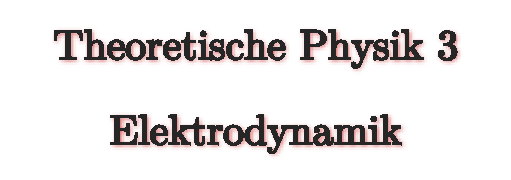
\includegraphics{images/Titel.pdf}}
\subtitle{Wintersemester 2021/2022}
\date{}
\author{von Kyano Levi\\bei Professor Holger Stark}

% -----------------------------------
% -----------------------------------
% -----------------------------------

\begin{document}

\frontmatter
\maketitle


\tableofcontents

% -----------------------------------
% -----------------------------------

\mainmatter
% !TEX root = Theo_III.tex

\chapter{Einleitung\label{einleitung}}

\section{Geschichte}

\begin{itemize}
	\item \textbf{1785} \textendash{} Charles Augustin de Coulomb: Entdeckung des Coulombsches Gesetzes.

	\item \textbf{1800} \textendash{} Alessandro Volta: Erfindung der erstern Batterie, die Voltasche Säule.

	\item \textbf{1820} \textendash{}  Hans Christian \O{}rsted: Das \O{}rstedsche Gesetz beschreibt, dass elektrische Ströme ein Magnetfeld erzeugen.

	\item \textbf{1820-25} \textendash{}   André-Marie Ampère: Entdeckung der Grundlagen der Magnetostatik durch Messungen.

	\item \textbf{1831} \textendash{}  Michael Faraday: Beschreibung der magnetischen Induktion.

	\item \textbf{1852} \textendash{}  Michael Faraday: Formulierung des Nahwirkungsstandpunktes (Beschreibung elektrischer Phänomene über Felder statt Kräfte).

	\item \textbf{1864} \textendash{} James Clerk Maxwell: Formulierung der Maxwell-Gleichungen als fundamentale Feldgleichungen des elektromagnetischen Feldes und Nutzung von elektrischen und magnetischen Hilfsfeldern für die physikalische Beschreibung in Materie sowie Äußerung der Vermutung, dass Licht eine elektromagnetische Welle ist.

	\item \textbf{1886} \textendash{} Heinrich Hertz: Nachweis elektromagnetischer Wellen und Postulierung eines Äthers als hypothetisches Ausbreitungsmedium.

	\item \textbf{1881} \textendash{} Michelson-Morley-Experiment: Konstanz der Lichtgeschwindigkeit unabhängig von Beobachter und Quelle ${\Rightarrow}$ ein absolutes Bezugssystem Äther existiert nicht.

	\item \textbf{1905} \textendash{} Albert Einstein: spezielle Relativitätstheorie.

\end{itemize}





\section{Inhalt}

Der Inhalt dieser Vorlesung gliedert sich in folgende Abschnitte:

\begin{itemize}
	\item Einleitung

	\item Elemente der Vektoranalysis

	\item Elektrostatik

	\item Elektrische Felder in Materie

	\item Magnetostatik

	\item Grundgleichungen der Elektrodynamik: Die Maxwellschen Gleichungen

	\item Spezielle Relativitätstheorie

	\item Ebene elektromagnetische Wellen

	\item Elektromagnetische Felder bei vorgegebenen Ladungen und Strömen
\end{itemize}



\section{Grundlegende Konstanten der Elektrodynamik}

Für Konstanten deren Wert per Definition festgelegt wurde, wird ein $\equiv $-Zeichen verwendet.


\begin{table}[H]
	\centering
	\begin{tabular}{|l|l|} \hline
		\textbf{Konstante}         & \textbf{Wert}                                                     \\\hline
		Vakuumlichtgeschwindigkeit & \centering\arraybackslash{}$c_{0}\equiv \SI{299792458}{\m\per\s}$ \\
		Elektrische Feldkonstante  & $\varepsilon _{0}=\SI{8,8541878128e-12}{\A\s\per\V\per\m}$        \\
		Magnetische Feldkonstante  & $\mu _{0}=\SI{1,25663706212e-6}{\N\per\square\A}$                 \\
		\hline
	\end{tabular}
\end{table}




\section{Grundlegende Formeln der Elektrodynamik}

Maxwellsche Feldgleichungen
\begin{equation*}
	\nabla \cdot \vec {D}=\rho _{f},\quad\nabla \cdot \vec {B}=0,\quad\nabla \times \vec {E}=-\frac{\partial \vec {B}}{\partial t},\quad\nabla \times \vec {H}=\vec {j}_{f}+\frac{\partial \vec {D}}{\partial t}
\end{equation*}
Materialgleichungen
\begin{equation*}
	\vec {D}=\varepsilon _{0}\vec {E}+\vec {P},\quad \vec {B}=\mu _{0}\left(\vec {H}+\vec {M}\right)
\end{equation*}
In linearen und isotropen Medien gilt
\begin{equation*}
	\vec {D}=\varepsilon _{0}\varepsilon _{r}\vec {E},\quad \vec {B}=\mu _{0}\mu _{r}\vec {H}
\end{equation*}
Im Vakuum gilt
\begin{equation*}
	\vec {D}=\varepsilon _{0}\vec {E}, \quad\vec {B}=\mu _{0}\vec {H}
\end{equation*}
Relationen von Lichtgeschwindigkeit, Feldkonstanten und Brechungsindex:
\begin{align*}
	c_{0} & =\frac{1}{\sqrt{\varepsilon _{0}\mu _{0}}} \\
	n     & =\frac{c_{0}}{c}
\end{align*}
In linearen, isotropen Medien gilt
\begin{equation*}
	n=\sqrt{\varepsilon _{0}\mu _{0}}
\end{equation*}
Gradient
\begin{equation*}
	\nabla \frac{1}{r}=-\frac{\vec {r}}{r^{3}}
\end{equation*}
Elektrisches Potential und elektrisches Feld:
\begin{equation*}
	\vec {E}=-\nabla \phi ,\quad \phi \left(\vec {r}\right)=\frac{1}{4\pi \varepsilon _{0}}\int \frac{\rho \left(\vec {r}'\right)}{\left| \vec {r}-\vec {r}'\right| }\diff ^{3}\vec {r}'
\end{equation*}

% !TEX root = Theo_III.tex


\chapter{Elemente der Vektoranalysis\label{elemente_der_vektoranalysis}}

\section{Vektoranalysis}

\subsection{Gradient und Nabla-Operator}

Der Gradient eines skalaren Feldes $U$ ist definiert über das totale Differential:
\begin{equation*}
	\diff U=\grad U\cdot \diff \vec {r}=\nabla U\cdot \diff \vec {r}
\end{equation*}
Der Gradient steht senkrecht auf den Äquipotentiallinien. Für kartesische Koordinaten gilt
\begin{equation*}
	\nabla =\vec {e}_{x}\frac{\partial }{\partial x}+\vec {e}_{y}\frac{\partial }{\partial y}+\vec {e}_{z}\frac{\partial }{\partial z}=\sum _{i}\vec {e}_{i}\nabla _{i},
\end{equation*}
während für krummlinige allgemein gilt, dass
\begin{equation*}
	\nabla =\sum _{i}\vec {e}_{i}\frac{1}{\left| \partial \vec {r}/\partial x_{i}\right| }\frac{\partial }{\partial x_{i}}.
\end{equation*}
\subsection{Divergenz eines Vektorfeldes\label{ref-007}}

Die Divergenz eines Vektorfeldes $\vec {a}$ wird beschrieben durch
\begin{equation*}
	\divg \vec {a}\left(\vec {r}\right)=\nabla \cdot \vec {a}\left(\vec {r}\right).
\end{equation*}
Sie gibt die Quellenhaftigkeit von $\vec {a}$ an. In kartesischen Koordinaten ist $\divg \vec {a}=\sum _{i}\nabla _{i}a_{i}$.



\begin{figure}[htb]
	\centering
	\tfigVolumeWithNormal
	\caption{Volumen $V$ mit Oberflächennormale $\hat{\vec{n}}$. }
	\label{fig:volume_with_normal}
\end{figure}

Betrachte zum Verständnis ein kleines Volumen $ V$ bei $\vec {r}$. Die Normalen $\hat{\vec {n }}$ zeigen überall nach außen (siehe \Abbref{fig:volume_with_normal}).
Der Fluss aus $V$ heraus ist gegeben durch
\begin{equation*}
	q\left(r\right) V,
\end{equation*}
wobei $q\left(r\right)=\divg \vec {a}$. Wir können sagen, dass
\begin{align*}
	q\left(\vec {r}\right)=\divg \vec {a}=\begin{cases} >0, & \text{Quelle von }\vec {a}                       \\
              <0, & \text{Senke von }\vec {a}                        \\
              =0, & \text{was reinflie\ss{}t},\text{flie\ss{}t raus}
	                                      \end{cases} .
\end{align*}



\subsection{Rotation eines Vektorfeldes}

Die Rotation eines Vektorfeldes $\vec {a}$ ist definiert als
\begin{equation*}
	\rot \vec {a}\left(\vec {r}\right)=\nabla \times \vec {a}\left(\vec {r}\right)
\end{equation*}


\begin{figure}[htb]
	\centering
	%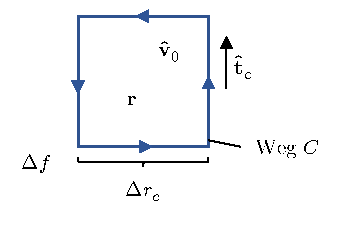
\includegraphics{vecanaylsis_curl.pdf}
	\tfigAreaWithCurveAndNormal
	\caption{Die Kurve $C$ mit Tangentialvektor $\hat{\vec{t}}$ schließt die Fläche $A$ mit Normalenvektor $\hat{\vec{n}}$ ein. }
	\label{fig:area_with_curve_normal}
\end{figure}

und es wird auch als das Wirbelfeld von $\vec {a}$ bezeichnet. Wieder ist die Darstellung in kartesischen Koordinaten einfach: $\left(\rot \vec {a}\right)_{i}=\varepsilon _{ijk}\partial _{{x_{j}}}a_{k}$.

Wir schauen uns ein kleines orientiertes Flächenelement $\vec F$ an, wie in \Abbref{fig:area_with_curve_normal} dargestellt. Dann ist die Verwirbelung/Zirkulation um $\vec F$
\begin{equation*}
	\sum _{C}\vec {a}\cdot \hat{\vec {t}}_{C}\Delta  r_{C}=\rot \vec {a}\cdot  \vec F
\end{equation*}
mit Tangentialvektor $\hat{\vec {t}}_{C}$ und Parallelkomponente $\vec {a}\cdot \hat{\vec {t}}_{C}$. Wir bezeichnen $\vec {\omega }=\rot \vec {a}$ als lokale Wirbelstärke.

Allgemein gilt, dass Gradientenfelder wirbelfrei sind,
\begin{equation*}
	\vec {a}=\grad U\equivalence \rot \vec {a}=0\quad\mathrm{bzw.}\quad  \rot \left(\grad U\right)=0
\end{equation*}
und Wirbelfelder quellenfrei sind,
\begin{equation*}
	\divg \vec {B}=0\equivalence \vec {B}=\rot \vec {A}\quad\mathrm{bzw.}\quad  \divg \left(\rot \vec {A}\right)=0.
\end{equation*}
Wir definieren ferner den Laplace-Operator als
\begin{equation*}
	\Delta  \equiv \nabla ^{2}\equiv \nabla \cdot \nabla ,
\end{equation*}
für den in kartesischen Koordinaten gilt:
\begin{equation*}
	\nabla ^{2}=\partial _{x}^{2}+\partial _{y}^{2}+\partial _{z}^{2}.
\end{equation*}
\subsection{Fundamentalsatz der Vektoranalysis (Helmholtz-Theorem)\label{ref-009}}

Das Helmholtz-Theorem besagt, dass Quellen und Wirbel ein Vektorfeld $\vec {a}\left(\vec {r}\right)$ eindeutig bestimmen. Ein Vektorfeld kann also in ein Rotationsfeld und ein Wirbelfeld aufgeteilt werden:
\begin{equation*}
	\vec {a}=\underset{\substack{
			\omega =\rot \vec {a}=\rot \vec {a}_{t} \\
			\divg \vec {a}_{t}=0 \\
			\text{Wirbel}!
		}}{\underbrace{\vec {a}_{t}}}+\underset{\substack{
			\rho =\divg \vec {a}=\divg \vec {a}_{l} \\
			\rot \vec {a}_{l}=0                     \\
			\text{Quellen}!
		}}{\underbrace{\vec {a}_{l}}}+\underset{\substack{
			\rot \vec {a}_{r}=\divg \vec {a}_{r}=0 \\
			\text{Randbedingungen}                 \\
			\hat{\vec {n }}\cdot \vec {a}=f\left(\vec {r}\right),\vec {r}\in \partial V
		}}{\underbrace{\vec {a}_{r}}}
\end{equation*}
Eine zusätzliche, sowohl quellen- als auch wirbelfreie Komponente kann vorkommen, um Randbedingungen zu erfüllen oder einen konstanten Untergrund zu addieren.

Ebene Transversalwellen ($e^{i\vec {k}\cdot \vec {r}}\perp \vec {k}$) sind zum Beispiel quellenfrei, ebene Longitudinalwellen ($e^{i\vec {k}\cdot \vec {r}}\parallel \vec {k}$) sind dagegen wirbelfrei, denn
\begin{equation*}
	\divg \left(e^{i\vec {k}\cdot \vec {r}}\right)=i\vec {k}\cdot e^{i\vec {k}\cdot \vec {r}},\quad \rot \left(e^{i\vec {k}\cdot \vec {r}}\right)=i\vec {k}\times e^{i\vec {k}\cdot \vec {r}}.
\end{equation*}




\section{Integration von Feldern}


\subsection{Linienintegrale}


\begin{equation*}
	\int _{C}\vec {a}\left(\vec {r}\right)\cdot \diff \vec {r}=\int _{C}\vec {a}\left(\vec {r}\left(s\right)\right)\cdot \frac{\diff \vec {r}}{\diff s}\diff s
\end{equation*}


\begin{figure}[htb]
	\centering
	\tfigLinienintegral
	\caption{Eine Kurve ist nach Bogenlänge $s$ parametrisiert, sodass für $s=0$ der Startpunkt $\vec r_0$ und für $s=1$ der Endpunkt $\vec r_1$ angenommen wird.
		Für einen auf der Kurve liegenden Punkt $\vec r$ ist der Tangentialvektor $\diff r$ eingezeichnet. }
	\label{fig:vecanaylsis_curve}
\end{figure}

Parameterdarstellung: $\vec {r}=\vec {r}\left(s\right)\rightarrow \diff \vec {r}=\frac{\diff \vec {r}}{\diff s}\diff s$ mit der Bogenlänge $s$.

Für rotationsfreie (Einschränkung, siehe Satz von Poincaré) Felder ist das Linienintegral zwischen zwei Punkten wegunabhängig:
\begin{equation*}
	\oint \vec {a}\cdot \diff \vec {r}=0\equivalence \vec {a}\left(\vec {r}\right)=\nabla \varphi \equivalence \rot \vec {a}=\vec {0}.
\end{equation*}


\subsection{Satz von Stokes}

\begin{equation*}
	\underset{\text{Fluss von }\rot \vec {a}~\text{durch} F}{\underbrace{ \int _{F}\rot \vec {a}\cdot \diff f}}=\underset{\text{Zirkulation von }\vec {a}~\text{entlang}~ C=\partial F}{\underbrace{\oint _{C=\partial F}\vec {a}\cdot \diff \vec {r}}}
\end{equation*}

\begin{figure}[htb]
	\centering
	\tfigHalbkugel
	\caption{}
	\label{fig:vecanaylsis_normal}
\end{figure}

Die Kurve $C$ ist dabei stets so orientiert, dass sie der Rechte-Hand-Regel folgt. Von außen (die Seite, nach der der Normalenvektor $\diff \vec {f}$ zeigt) betrachtet geht die Kurve gegen den Uhrzeigersinn.


\subsection{Satz von Gauß}

\begin{equation*}
	\underset{\text{Quellen von }\vec {a}~\mathrm{in} V}{\underbrace{ \int _{V}\divg \vec {a}\cdot \mathrm{dV}}}=\underset{\substack{
			\text{Fluss von }\vec {a}~\text{durch } \\
			\partial V \mathrm{aus}~V \text{heraus}
		}}{\underbrace{\int _{\partial V}\vec {a}\cdot \diff\vec f}}
\end{equation*}
Aus den Satz von Gauß abgeleiteten Formen:
\begin{itemize}
	\item $\vec {a}=g\vec {e}_{i}\rightarrow \int _{V}\frac{\partial }{\partial x_{i}}g\diff V=\int _{\partial V}g\diff f_{i}$

	\item $g=a_{j}\rightarrow \int _{V}\rot \vec {a}\diff V=\int _{\partial V}\diff \vec {f}\times \vec {a}$

	\item Greensche Identitäten (diese finden ihre Anwendung in der Potentialtheorie, hierzu wird $\nabla ^{2}\varphi $ verwendet). $\vec {a}_{1}=\varphi \nabla \psi , \vec {a}_{2}=\psi \nabla \varphi $.

	      \begin{enumerate}[a]
		      \setcounter{enumii}{14}

		      \item[o] 1. Identität: $\int \nabla \cdot \vec {a}_{1}\diff V$
			      \begin{equation*}
				      \int _{V}\left(\nabla \varphi \cdot \nabla \psi +\varphi \nabla ^{2}\psi \right)\diff V=\int _{\partial V}\varphi \nabla \psi \cdot \diff \vec f
			      \end{equation*}
		      \item[o] 2. Identität: $\int \left(\nabla \cdot \vec {a}_{1}-\nabla \cdot \vec {a}_{2}\right)\diff V$ (Greenscher Satz)
			      \begin{equation*}
				      \int _{V}\left(\varphi \nabla ^{2}\psi -\psi \nabla ^{2}\varphi \right)\diff V=\int _{\partial V}\left(\varphi \nabla \psi -\psi \nabla \varphi \right)\cdot \diff \vec f
			      \end{equation*}
	      \end{enumerate}
\end{itemize}

% !TEX root = Theo_III.tex

\chapter{Elektrostatik\label{elektrostatik}}

Die Elektrostatik behandelt elektrische Felder ruhender oder langsam bewegter elektrischer Ladungen. In den folgenden Kapiteln werden die Grundgesetze der Elektrostatik aus dem Coulomb-Gesetz abgeleitet.

\section{Bemerkungen zur elektrischen Ladung}

Es gibt zwei Arten von Ladungen: positive und negative Ladung. Die Ladung ist eine diskrete Größe und nimmt stets ein ganzzahliges Vielfaches der sogenannten Elementarladung $e_{0}$ an:
\begin{equation*}
	e_{0}=\SI{1.602176624e-19}{\coulomb}
\end{equation*}
Diese wurde zuerst bei dem Millikan-Versuch bestimmt. So trägt zum Beispiel das Proton die Ladung $+e_{0}$ und das Elektron die Ladung $-e_{0}$. Quarks haben zwar Bruchteile der Elementarladung, treten aber nie frei, sondern nur in Kombinationen auf, die ein Vielfaches der Elementarladung bilden.

Es gilt strenge Ladungserhaltung:
\begin{formal}
	In einem abgeschlossenen System bleibt die Summe aller Ladungen konstant.
\end{formal}
Eine Ladung auf einem infinitesimalen Raum wird als Punktladung bezeichnet. In der Elektrostatik und der Elektrodynamik wird häufig mit der Ladungsdichte $\rho $ gerechnet. Für eine einzige Punktladung $q$ (zum Beispiel ein Proton oder Elektron) am Ort $\vec {r}_{0}$ gilt für die Ladungsdichteverteilung
\begin{equation*}
	\rho \left(\vec {r}\right)=q\delta \left(\vec {r}-\vec {r}_{0}\right).
\end{equation*}
Daraus lässt sich die Ladungsdichte für viele Punktladungen $q_{i}$ an Orten $\vec {r}_{i}$ verallgemeinern:
\begin{equation*}
	\rho \left(\vec {r}\right)=\sum _{i}q_{i}\delta \left(\vec {r}-\vec {r}_{i}\right)
\end{equation*}
Im Grenzwert für kleinste Abstände kann man schließlich auch mit kontinuierlichen Ladungsdichten rechnen:
\begin{equation*}
	\rho \left(\vec {r}\right)=\frac{\diff Q}{\diff V}
\end{equation*}
Die gesamte Ladung in einem Volumen $V$ ist also
\begin{equation*}
	Q=\int _{V}\diff ^{3}\vec {r}\rho \left(\vec {r}\right).
\end{equation*}



\section{Coulombsches Gesetz und elektrisches Feld}

Im Alltag machen wir die Erfahrung, dass sich gleichnamige (also zum Beispiel zwei positive) Ladungen abstoßen, während zwischen ungleichnamigen Ladungen eine anziehende Kraft wirkt. Diese Kraft ist ein Vektor im Sinne der Newtonschen Mechanik und unterliegt also dem Superpositionsprinzip.


\subsection{Coulombsches Gesetz}

Die Kraft, die eine Ladung $q_{2}$ am Ort $\vec {r}_{2}$ auf eine Ladung $q_{1}$ am Ort $\vec {r}_{1}$ ausübt (siehe \Abbref{fig:coulomb_point_charges}), berechnet sich durch
\begin{equation}
	\label{3.1}
	\boxed{\vec {F}_{1}=kq_{1}q_{2}\frac{\vec {r}_{1}-\vec {r}_{2}}{\left| \vec {r}_{1}-\vec {r}_{2}\right| ^{3}}=-\vec {F}_{2}.}
\end{equation}
Dieser Zusammenhang ist als Coulombsches Gesetz bekannt und wurde experimentell gefunden. Die Proportionalitätskonstante $k$ ist dabei
\begin{equation*}
	k=\frac{1}{4\pi \varepsilon _{0}}. 
\end{equation*}

\begin{figure}[htb]
	\centering
	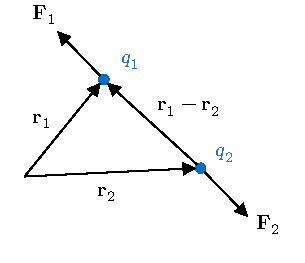
\includegraphics{coulomb_point_charges.pdf}
	\caption{Die Kraft auf zwei Punktladungen $q_1$ und $q_2$ an Orten $\vec r_1$ und $\vec r_2$ wird durch das Coulombsche Gesetz beschrieben und ist invers proportional zum Qudrat des Abstands $\left|\vec r_1-\vec r_2\right|$. }
	\label{fig:coulomb_point_charges}
\end{figure}

mit Dielektrizitätskonstante $\varepsilon _{0}=\SI{8,8541878128e-12}{\farad\per\m}$. Das Coulombsche Gesetz hat die gleiche Form wie das Newtonsche Gravitationsgesetz, aber hier kann die Kraft auch abstoßend wirken, weil die Ladung anders als die Masse negativ sein kann. Genauso wie beim Gravitationsgesetz ist die Kraft antiproportional zum Quadrat des Abstands der Ladungen.\footnote{Es ist möglich, dass die Proportionalität nicht exakt $\vec {F}\propto r^{-2}$ ist, aber es ist durch Experimente bestätigt worden, dass für einen Ansatz $F\propto r^{-2-\varepsilon }$ zumindest $\varepsilon <3\cdot 10^{-16}$ ist und für einen Ansatz $F\propto e^{-\frac{r}{\xi }}r^{-2}$ (siehe sogenanntes Yukawa-Potential) wenigstens $\xi >\SI{1e8}{\m}$. }

Mithilfe des Coulombschen Gesetzes können wir nach dem Superpositionsprinzip die Kraft auf eine Testladung $q_{0}$ am Ort $\vec {r}_{0}$ durch mehrere Ladungen $q_{i}$ bestimmen:
\begin{equation}
	\label{3.2}
	\vec {F}=\frac{q_{0}}{4\pi \varepsilon _{0}}\sum _{i}q_{i}\frac{\vec {r}_{0}-\vec {r}_{i}}{\left| \vec {r}_{0}-\vec {r}_{i}\right| ^{3}}
\end{equation}
Dieser Ansatz ist der Fernwirkungsstandpunkt (die Kraft wirkt über die Ferne hinweg). Seit Veröffentlichung der Relativitätstheorie ist aber bekannt, dass sich nichts schneller als mit Vakuumlichtgeschwindigkeit bewegen kann \textendash{} also auch keine Kraftwirkung. 

Daher führt man den sogenannten Nahwirkungsstandpunkt ein, bei dem man man ein elektrisches Feld $\vec {E}$ betrachtet, das durch Ladungen $q_{i}$ erzeugt wird ($\vec {E}$ zeigt weg von positiven Ladungen und hin zu den negativen):
\begin{equation}
	\vec {E}\left(\vec {r}\right)=\frac{1}{4\pi \varepsilon _{0}}\sum _{i}q_{i}\frac{\vec {r}_{0}-\vec {r}_{i}}{\left| \vec {r}_{0}-\vec {r}_{i}\right| ^{3}},\quad \vec {E}\left(\vec {r}\right)=\frac{1}{4\pi \varepsilon _{0}}\int \rho \left(\vec {r}'\right)\frac{\vec {r}-\vec {r}'}{\left| \vec {r}-\vec {r}'\right| ^{3}}\diff ^{3}\vec {r}'
\end{equation}
Damit ergibt sich die folgende Kraft auf eine Testladung $q_{0}$:
\begin{equation}
	\vec {F}=q_{0}\vec {E}\left(\vec {r}_{0}\right)
\end{equation}


\section{Feldgleichungen der Elektrostatik}

\subsection{Grundlagen}

Wir definieren zunächst das elektrostatische Potential:
\begin{equation}
	\label{3.3}
	\boxed{\vec {E}=-\nabla \phi ,\quad \phi \left(\vec {r}\right)=\frac{1}{4\pi \varepsilon _{0}}\int \frac{\rho \left(\vec {r}'\right)}{\left| \vec {r}-\vec {r}'\right| }\diff ^{3}\vec {r}'}
\end{equation}
Weil $\vec {E}$ ein Potentialfeld ist, ist $\rot \vec {E}=0$. Das elektrostatische Feld ist also wirbelfrei.

Zum Beispiel ist das Potential einer Punktladung $\rho \left(\vec {r}\right)=q\delta \left(\vec {r}-\vec {r}_{0}\right)$ nach obiger Formel\footnote{Hinweis: Es gilt
	\begin{equation*}
		\nabla \frac{1}{\left| \vec {r}-\vec {r}\mathrm{'}\right| }=-\frac{1}{\left| \vec {r}-\vec {r}\mathrm{'}\right| ^{2}}\nabla \left| \vec {r}-\vec {r}\mathrm{'}\right| \overset{\nabla r=\frac{\vec {r}}{r}=\hat{\vec {r}}}{=}-\frac{\vec {r}-\vec {r}\mathrm{'}}{\left| \vec {r}-\vec {r}\mathrm{'}\right| ^{3}}
	\end{equation*}
}:
\begin{equation*}
	\phi \left(\vec {r}\right)=\frac{1}{4\pi \varepsilon _{0}}\frac{q}{\left| \vec {r}-\vec {r}_{0}\right| }
\end{equation*}
Die Quellen des elektrischen Feldes werden durch die Divergenz von $\vec E$ beschrieben,
\begin{equation*}
	\divg \vec {E}=-\nabla ^{2}\phi =-\frac{1}{4\pi \varepsilon _{0}}\int \rho \left(\vec {r}\mathrm{'}\right)\underset{\overset{!}{=}-4\pi \delta \left(\vec {r}-\vec {r}\mathrm{'}\right)}{\underbrace{\nabla ^{2}\frac{1}{\left| \vec {r}-\vec {r}\mathrm{'}\right| }}}\diff ^{3}r\mathrm{'}=\frac{1}{\varepsilon _{0}}\rho \left(\vec {r}\right).
\end{equation*}
\subsection{Feldgleichungen der Elektrostatik\label{ref-020}}

Die soeben gefundenen Zusammenhänge werden als Feldgleichungen der Elektrostatik bezeichnet:
\begin{align}
	\label{3.4}
	\Aboxed{\divg \vec {E}&=\frac{1}{\varepsilon _{0}}\rho \left(\vec {r}\right)} \\
	\label{3.5}
	\Aboxed{\rot \vec {E}&=0}
\end{align}
Die erste Gleichung wird als Gaußsches Gesetz bezeichnet und beschreibt die elektrische Ladung als Quelle des elektrischen Feldes. Die zweite beschreibt die Wirbelfreiheit des elektrostatischen Feldes.

Mit $\vec {D}=\varepsilon _{0}\vec {E}$ im Vakuum kann man das Gaußsche Gesetz auch umformulieren zu
\begin{equation}
	\label{3.6}
	\divg \vec {D}=\rho \left(\vec {r}\right).
\end{equation}
Zu beiden Feldgleichungen gibt es integrale Formulierungen:
\begin{equation*}
	\int _{V}\diff ^{3}\vec r\divg \vec {E}=\int _{\partial V}\vec {E}\cdot \diff \vec {f}=\frac{1}{\varepsilon _{0}}\int \diff ^{3}\vec r\rho \left(\vec {r}\right)\implication \boxed{\int _{\partial V}\vec {E}\cdot \diff \vec f=\frac{1}{\varepsilon _{0}}Q}
\end{equation*}
\begin{formal}
    Der Fluss aus einem Volumen $V$ heraus ist proportional zu der Gesamtladung. Die elektrische Ladungsdichte ist die Quelle des elektrischen Feldes. 
\end{formal}
Betrachte als Beispiel eine Punktladung, die das Feld $\vec {E}=\frac{1}{4\pi \varepsilon _{0}}q\frac{\vec {r}-\vec {r}_{0}}{\left| \vec {r}-\vec {r}_{0}\right| ^{3}}=\frac{1}{4\pi \varepsilon _{0}}q\frac{\hat{\vec {R}}}{R^{2}}$ erzeugt:
\begin{equation*}
	\int _{\partial V_{K}}\vec {E}\cdot \diff \vec {f}=\frac{q}{4\pi \varepsilon _{0}}\int _{\partial V_{K}}\frac{\hat{\vec {R}}}{R^{2}}\cdot \hat{\vec {R}}R^{2}\diff \Omega  =\frac{q}{4\pi \varepsilon _{0}}\int _{\partial V_{K}}\diff \Omega  =\frac{q}{\varepsilon _{0}}
\end{equation*}
Für die andere Feldgleichung betrachten wir das Arbeitsintegral, also die von einer Punktladung $q$ verrichtete Arbeit gegen die elektrische Kraft $\vec F_{\mathrm{el}}=q\vec {E}$.
\begin{equation*}
	W=-q\int _{C}\vec {E}\cdot \diff \vec {r}=q\int _{C}\nabla \phi \cdot \diff \vec {r}=q\int _{C}\diff \phi =q\left[\phi \left(2\right)-\phi \left(1\right)\right]
\end{equation*}
Insbesondere gilt
\begin{equation}
	\label{3.7}
	\oint \vec {E}\cdot \diff \vec {r}=0
\end{equation}

\begin{formal}
	Die Feldlinien des elektrostatischen Feldes sind nicht geschlossen, es gibt keine Zirkulation in der Elektrostatik, $\rot \vec {E}=0$.
\end{formal}



\subsection{Potentialgleichung}

Aus dem Gaußschen Gesetz können wir die folgende Poisson-Gleichung ableiten, die für $\rho =0$ zu einer Laplace-Gleichung wird:
\begin{equation}
	\label{3.8}
	\boxed{\nabla ^{2}\phi =-\frac{1}{\varepsilon _{0}}\rho }
\end{equation}
Zur Lösung einer linearen Differentialgleichung können wir die Methode der Greenschen Funktion verwenden. Dabei drücken wir die Lösung allgemein als Faltung der Ladungsdichte mit einer sogenannten Greenschen Funktion aus,
\begin{equation}
	\label{3.9}
	\phi \left(\vec {r}\right)=\int G\left(\vec {r}-\vec {r}'\right)\rho \left(\vec {r}'\right)\diff ^{3}\vec {r}'.
\end{equation}
Durch Vergleich mit der Bestimmungsgleichung des elektrischen Potentials können wir die Greensche Funktion für diese Differentialgleichung ablesen:
\begin{equation}
	\label{3.10}
	G\left(\vec {r}-\vec {r}'\right)=\frac{1}{4\pi \varepsilon _{0}}\frac{1}{\left| \vec {r}-\vec {r}'\right| }
\end{equation}
Insbesondere gilt für eine Punktladung $\rho \left(\vec {r}\right)=\delta \left(\vec {r}-\vec {r}_{0}\right)$, dass $\phi \left(\vec {r}\right)=G\left(\vec {r}-\vec {r}_{0}\right)$ und damit, dass
\begin{equation*}
	\nabla ^{2}\frac{1}{\left| \vec {r}-\vec {r}_{0}\right| }=-4\pi \delta \left(\vec {r}-\vec {r}_{0}\right).
\end{equation*}



\subsection{Feldlinien}

\begin{figure}[htb]
	\centering
	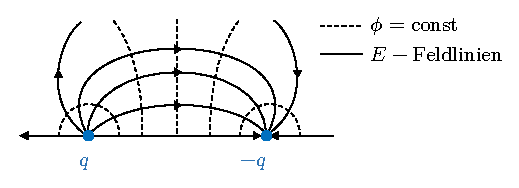
\includegraphics{dipole_field_potential.pdf}
	\caption{Äquipotentiallinien und elektrische Feldlinien von zwei ungleichnamigen Ladungen. }
	\label{fig:dipole_field_potential}
\end{figure}

Als Äquipotentiallinien bzw. -flächen werden die Linien/Flächen gleichen Potentials, $\phi =\text{const}$ bezeichnet. Die Feldlinien stehen senkrecht auf den Äquipotentialflächen, weil $\vec {E}\left(\vec {r}\right)=-\nabla \phi $. In \Abbref{fig:dipole_field_potential} sind die Äquipotentiallinien und die Feldlinien einer positiven und einer negativen Ladung dargestellt. 

\subsection{Elektrostatische Energie}

Die potentielle Energie einer Ladung $q$ am Ort $\vec {r}$ im Feld $\vec {E}=-\nabla \phi $ ist definiert über einen Referenzpunkt $\phi _{1}=0$, der zum Beispiel im Unendlichen liegt (aber je nach Anwendung auch an anderen Punkten liegen kann):
\begin{equation}
	\label{3.11}
	U\left(\vec {r}\right)=q\phi \left(\vec {r}\right)
\end{equation}
Zum Beispiel ist die potentielle Energie von zwei Punktladungen
\begin{equation*}
	U=q_{1}\phi _{2}=\frac{1}{4\pi \varepsilon _{0}}\frac{q_{1}q_{2}}{\left| \vec {r}_{1}-\vec {r}_{2}\right| }.
\end{equation*}
Die elektrostatische Energie $U$ von $N$ Punktladungen im eigenen Feld kann dann in zwei Schritten bestimmt werden.
\begin{itemize}
	\item Bestimme die Energie von $q_{i}$ im Feld von $q_{j}$ ($j=1,\ldots ,i-1$):
	      \begin{equation*}
		      U_{i}\left(\vec {r}_{i}\right)=q_{i}\sum _{j=1}^{i-1}\phi _{j}=\frac{q_{i}}{4\pi \varepsilon _{0}}\sum _{j=1}^{i-1}\frac{q_{j}}{\left| \vec {r}_{i}-\vec {r}_{j}\right| }
	      \end{equation*}
	\item Bringe $N$ Ladungen sukzessive an ihren Ort:
	      \begin{equation*}
		      U=\sum _{i=2}^{N}U_{i}\left(\vec {r}_{i}\right)=\frac{1}{4\pi \varepsilon _{0}}\sum _{i=2}^{N}\sum _{j=1}^{i-1}\frac{q_{i}q_{j}}{\left| \vec {r}_{i}-\vec {r}_{j}\right| }=\frac{1}{8\pi \varepsilon _{0}}\sum _{i\neq j}^{N}\frac{q_{i}q_{j}}{\left| \vec {r}_{i}-\vec {r}_{j}\right| }
	      \end{equation*}

\end{itemize}
Für eine kontinuierliche Ladungsverteilung ergibt sich
\begin{equation*}
	U=\frac{1}{8\pi \varepsilon _{0}}\int \diff ^{3}\vec {r}\diff ^{3}\vec {r}'\frac{\rho \left(\vec {r}\right)\rho \left(\vec {r}'\right)}{\left| \vec {r}-\vec {r}'\right| }=\frac{1}{2}\int \diff ^{3}\vec {r}\rho \left(\vec {r}\right)\phi \left(\vec {r}\right)
\end{equation*}
Bemerkungen:
\begin{itemize}
	\item Den zusätzlichen Faktor von $\frac{1}{2}$ erhält man, weil $\phi \left(\vec {r}\right)$ von $\rho \left(\vec {r}\right)$ selbst erzeugt wird und die gegenseitige Wirkung von je zwei Ladungen die gleiche ist.

	\item Für beschränkte $\rho $ ist $\vec {r}\rightarrow \vec {r}'$ wohl definiert, da $\diff ^{3}r=r^{2}\diff r\diff \Omega  $.


\end{itemize}
Es ist auch möglich, die Energie durch das Feld $\vec {E}\left(\vec {r}\right)$ auszudrücken:
\begin{equation*}
	U=\frac{\varepsilon _{0}}{2}\int \diff ^{3}\vec {r}\phi \nabla ^{2}\phi \overset{\text{partielle Int}.}{=}\frac{\varepsilon _{0}}{2}\int \diff ^{3}\vec {r}\nabla \phi \cdot \nabla \phi =\frac{\varepsilon _{0}}{2}\int \diff ^{3}\vec {r}\left| \vec {E}\right| ^{2}
\end{equation*}
Damit lässt sich die Energiedichte in der Elektrostatik folglich schreiben als
\begin{equation*}
	u\left(\vec {r}\right)=\frac{\varepsilon _{0}}{2}\left| \vec {E}\left(\vec {r}\right)\right| ^{2}=\frac{1}{2}\vec {E}\cdot \vec {D}.
\end{equation*}



\subsection{Homogen geladene Kugel}

\begin{figure}[htb]
	\centering
	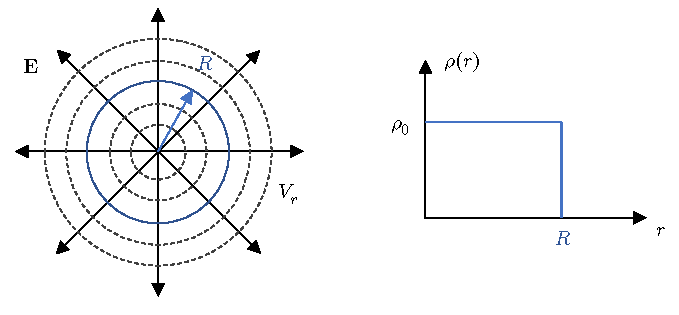
\includegraphics{homogenously_charged_ball.pdf}
	\caption{Links: Äquipotentiallinien und elektrische Feldlinien einer homogen geladenen Kugel mit Radius $R$. Rechts: Die Ladungsdichte ist konstant $\rho_0$ innerhalb ($r<R$) und gleich 0 außerhalb der Kugel. }
	\label{fig:homogenously_charged_ball}
\end{figure}

Auf der homogen geladenen Kugel $V_{r}$ ist die Ladungsdichte $\rho \left(\vec {r}\right)$ innerhalb der Kugel konstant $\rho _{0}$ und außerhalb der Kugel gleich $0$ (siehe \Abbref{fig:homogenously_charged_ball}). Das Problem ist kugelsymmetrisch und hängt nur von der Radialrichtung ab.



\begin{figure}[htb]
	\centering
	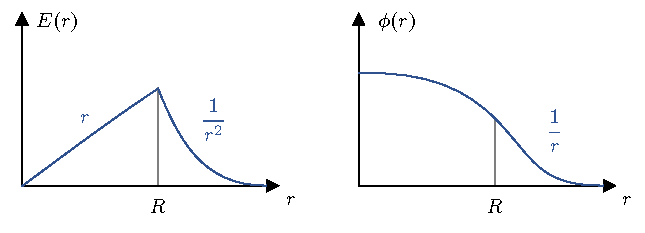
\includegraphics{homogenously_charged_ball_field_potential.pdf}
	\caption{Links: Elektrisches Feld einer homogen geladenen Kugel. Das Feld steigt im Inneren linear an und fällt im Äußeren mit $r^{-2}$ ab. Rechts: Das Potential fällt im Äußeren genauso ab wie das Potential einer Punktladung. }
	\label{fig:homogenously_charged_ball_field_potential}
\end{figure}

Feld und Potential können zum Beispiel über das Gaußsche Gesetz berechnet werden:
\begin{align*}
	\int _{{V_{r}}}\diff ^{3}r'\frac{\rho \left(r\right)}{\varepsilon _{0}}&=\int _{{V_{r}}}\diff ^{3}r'\divg \vec {E}=\int _{\partial {V_{r}}}\vec {E}\cdot \diff \vec {f}\implication 4\pi r^{2}E\left(r\right)=\frac{1}{\varepsilon _{0}}\int _{0}^{r}\diff r'r'^{2}\rho \left(r'\right) \\
	\Rightarrow E\left(r\right)&=\frac{Q}{4\pi \varepsilon _{0}}
	\begin{cases} \frac{r}{R^{2}}, & r<R     \\
          \frac{1}{r^{2}}, & r\geq R
	\end{cases} \quad\xrightarrow{\text{Integration}}\quad \phi \left(r\right)=\frac{Q}{4\pi \varepsilon _{0}}
	\begin{cases} \frac{1}{R}\left(\frac{3}{2}-\frac{r^{2}}{2R^{2}}\right), & r<R     \\
          \frac{1}{r},  & r\geq R
	\end{cases}
\end{align*}
Beide Größen sind in \Abbref{fig:homogenously_charged_ball_field_potential} dargestellt. Bemerkenswert ist, dass für $r\geq R$ das elektrische Feld $\vec {E}\left(\vec {r}\right)=E\left(r\right)\cdot \vec {e}_{r}$ gerade dem Feld einer Punktladung $Q$ im Mittelpunkt der Kugel entspricht.

Es soll nun die Energiedichte $u\left(\vec {r}\right)$ für die homogen geladene Kugel berechnet werden:
\begin{align*}
	u\left(\vec {r}\right)=\frac{\varepsilon _{0}}{2}\left| \vec {E}\right| ^{2}=\frac{Q^{2}}{32\pi ^{2}\varepsilon _{0}}\begin{cases} \frac{r^{2}}{R^{6}}, & r<R     \\
              \frac{1}{r^{4}},     & r\geq R
    \end{cases}
\end{align*}
Daraus ergibt sich die elektrostatische Energie ("`Selbstenergie`` einer homogen geladenen Kugel)
\begin{equation*}
	U=4\pi \int _{0}^{\infty }\diff ru\left(r\right)r^{2}=\frac{1}{4\pi \varepsilon _{0}}\frac{3}{5}\frac{Q^{2}}{R}.
\end{equation*}
Diese Rechnung lässt über die Ruheenergie eines Elektrons eine Abschätzung für den Elektronenradius zu (sogenannter klassischer Elektronenradius):
\begin{equation*}
	U\overset{!}{=} m_{e}c^{2}\approx \SI{0.5}{\mega\eV}\implication R_{e}= \SI{1,7e-15}{\m}
\end{equation*}
Allerdings liegt die Compton-Wellenlänge $\lambda _{e}=\frac{h}{m_{e}c}=\SI{2e-12}{\m}$ schon weit über diesem Radius, sodass Quanteneffekte hier nicht vernachlässigbar sind.



\subsection{Extremalprinzip und Kapazitäten}

\begin{formal}
	In der Elektrostatik sind Leiter stets Äquipotentialflächen, d.h. $\phi =\text{const}$ und daher $\vec {E}=-\nabla \phi =\vec {0}$ entlang des Leiters. Sonst würde ein Strom fließen, weil sich die freien Elektronen im Leiter aufgrund des nicht-verschwindenden Feldes bewegen würden.
\end{formal}

\begin{figure}[htb]
	\centering
	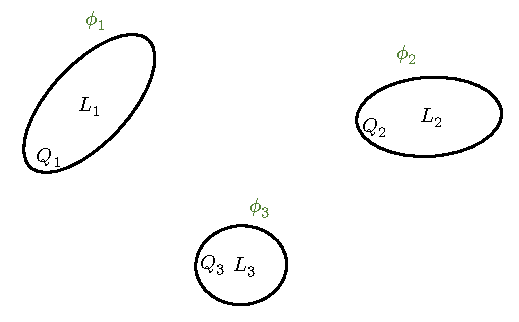
\includegraphics{three_conductors.pdf}
	\caption{Konfiguration von elektrischen Leitern $L_i$ mit Ladungen $Q_i$ und Potentialen $\phi_i$. }
	\label{fig:three_conductors}
\end{figure}

Betrachte den Fall von $n$ Leitern mit Volumina $L_{i}$, einer Ladung $Q_{i}$ und den Potentialen $\phi _{i}$, wie schematisch in \Abbref{fig:three_conductors} gezeigt.

Es soll untersucht werden, wie aus der Ladungsverteilung die Potentiale und das elektrische Feld bestimmt werden können.
\begin{formal}
		\textbf{Theorem von Thomson:}
		
		Die Ladungsdichten $\rho _{i}\left(\vec {r}\right)$ in Leitern $i$ stellen sich so ein, dass die Gesamtenergie minimal wird.
\end{formal}
Beweis:
\begin{equation*}
	U=\frac{1}{8\pi \varepsilon _{0}}\sum _{ij}\int _{L_{i}}\diff ^{3}\vec {r}_{i}\int _{L_{j}}\diff ^{3}\vec {r}_{j}\frac{\rho _{i}\left(\vec {r}_{i}\right)\rho _{j}\left(\vec {r}_{j}\right)}{\left| \vec {r}_{i}-\vec {r}_{j}\right| }
\end{equation*}
Minimierung unter der Nebenbedingung $\int _{{L_{i}}}\diff ^{3}\vec {r}\rho _{i}\left(\vec {r}\right)=Q_{i}$ führt auf
\begin{equation*}
	\frac{\partial }{\partial \rho _{k}\left(\vec {r}\right)}\left(U-\sum _{i}\phi _{i}\int _{L_{i}}\diff ^{3}\vec {r}_{i}\rho _{i}\left(\vec {r}\right)\right)=0
\end{equation*}
wobei in Voraussicht die Lagrange-Parameter als $\phi _{i}$ bezeichnet werden, weil sich mit
\begin{equation*}
    \partial _{{\rho _{k}}\left(\vec {r}\right)}\sum _{i}\int \rho _{i}\left(\vec {r}\right)f_{i}\left(\vec {r}\right)\diff ^{3}r=f_{k}\left(\vec {r}\right)
\end{equation*}
ergibt, dass
\begin{equation*}
	\phi _{k}=\frac{1}{4\pi \varepsilon _{0}}\sum _{j}\int _{L_{j}}\diff ^{3}\vec {r}_{j}\frac{\rho _{j}\left(\vec {r}_{j}\right)}{\left| \vec {r}_{k}-\vec {r}_{j}\right| },\quad \vec {r}_{k}\in L_{k}
\end{equation*}
was gerade der Bestimmungsgleichung für das Potential $\phi _{k}$ als Potential von $L_{k}$ entspricht. Da das Vorgehen der Minimierung der Gesamtenergie auf das richtige Potential führt, ist das Theorem bestätigt.



\subsubsectiona{Kapazitäten}

Die Potentiale $\phi _{i}$ lassen sich linear über die Ladungen $Q_{i}$ zerlegen,
\begin{equation*}
	\phi _{i}=\sum _{j}p_{ij}Q_{j},
\end{equation*}
weil einerseits gilt, dass $\nabla ^{2}\phi =-\rho /\varepsilon _{0}$ und andererseits $\phi $ linear in $\rho $ ist. Dieser Zusammenhang lässt sich invertieren,
\begin{equation*}
	Q_{i}=\sum _{j}C_{ij}\phi _{j},
\end{equation*}
wobei dann die Vorfaktoren $C_{ij}$ als Kapazitäten mit der Einheit $\left[C_{ij}\right]=\SI{1}{\coulomb\per\V}=\SI{1}{\farad}$ definiert werden. Aus dem Ausdruck für die elektrostatische Energie
\begin{equation*}
	U=\frac{1}{2}\sum _{i}\underset{Q_{i}=\sum _{j}C_{ij}\phi _{j}}{\underbrace{\int _{L_{i}}\diff ^{3}\vec {r}_{i}\rho _{i}\left(\vec {r}_{i}\right)\phi _{i}}}=\frac{1}{2}\sum _{ij}\phi _{i}C_{ij}\phi _{j}
\end{equation*}
folgt die Symmetrie $C_{ij}=C_{ji}$.

So gilt zum Beispiel für einen Plattenkondensator allgemein
\begin{equation*}
	C=\frac{Q}{V},\quad U=\frac{1}{2}CV^{2}=\frac{1}{2}QV
\end{equation*}
für einen Plattenkondensator mit parallelen Platten der Fläche $A$ und Abstand $d$
\begin{equation*}
	C=\varepsilon _{0}\varepsilon _{r}\frac{A}{d},
\end{equation*}
für einen Zylinderkondensator der Länge $L$ und mit Radien $r_{1}<r_{2}$
\begin{equation*}
	C=2\pi \varepsilon _{0}\varepsilon _{r}\frac{L}{\ln \frac{r_{2}}{r_{1}}}
\end{equation*}
und schließlich für einen Kugelkondensator mit Radien $r_{1}<r_{2}$
\begin{equation*}
	C=4\pi \varepsilon _{0}\varepsilon _{r}\left(\frac{1}{r_{1}}-\frac{1}{r_{2}}\right)^{-1}=4\pi \varepsilon _{0}\varepsilon _{r}\frac{r_{1}r_{2}}{d}.
\end{equation*}
\Abbref{fig:capacitors} bildet diese drei einfachen Kondensatorgeometrien ab. 


\begin{figure}[htb]
	\centering
	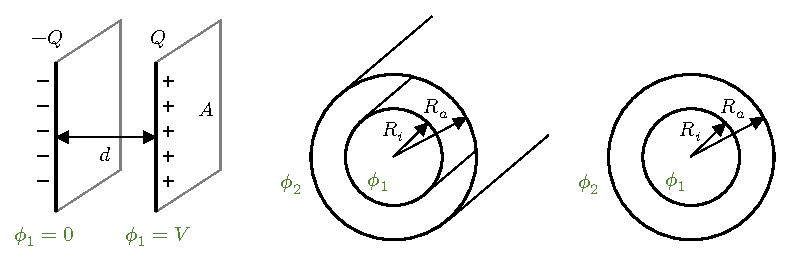
\includegraphics{capacitors.pdf}
	\caption{Schematische Darstellung eines Plattenkondensators mit parallelen, ebenen Platten (Links), eines Zylinderkondensators (Mitte) und eines Kugelkondensators (Rechts). Auf den Platten ist das Potential jeweils $\phi_1$ und $\phi_2$. }
	\label{fig:capacitors}
\end{figure}



\subsection{Maxwellscher Spannungstensor}

\section{Randbedingungen des elektrischen Feldes auf Grenzflächen\label{sec:randbedingungen_auf_grenzflaechen}}

 {\ldots}

\section{Randwertprobleme der Elektrostatik}

Meist sind bei der Lösung von elektrostatischen Problemen der Poisson-Gleichung
\begin{equation*}
	\nabla ^{2}\phi =-\frac{\rho }{\varepsilon _{0}}
\end{equation*}
in einem Volumen $V$ noch die Randbedingungen auf $\partial V$ zu berücksichtigen.

\subsection{Eindeutigkeit der Lösung}

Allgemein sind drei verschiedene Arten von Randbedingungen möglich. 

\begin{enumerate}
	\item Dirichlet-Randbedingung: Das Potential ist auf dem Rand vorgegeben, $\left.\hspace{0pt}\phi \right| _{\partial V}$.

	\item Neumann-Bedingung: Die Normalenableitung der Lösung wird auf dem Rand vorgegeben, $\vec {n}\cdot \left.\hspace{0pt}\nabla \phi \right| _{\partial V}=\left.\frac{\partial \phi }{\partial n}\right| _{\partial V}$

	\item Cauchy-Bedingung: $a\left(1\right)+b\left(2\right)$ ist vorgegeben.
\end{enumerate}

Zum Beispiel kommt die Dirichlet-Randbedingung bei Oberflächen von Leitern vor, von denen wir ja bereits wissen, dass dort das Potential konstant gleich $0$ ist.
\begin{formal}
	Für Dirichlet- und Neumann-Randbedingungen ist die Lösung der Poisson-Gleichung eindeutig.
\end{formal}
Der Beweis ist einfach, denn seien $\phi _{1}$ und $\phi _{2}$ zwei unterschiedliche Lösungen, dann erfüllt $\phi _{d}=\phi _{1}-\phi _{2}$ die Gleichung $\nabla ^{2}\phi _{2}=0$ mit der Randbedingung
\begin{align*}
	\begin{cases} \left.\phi _{d}\right| _{\partial V}                             & =0 \\
              \left.\frac{\partial \phi _{d}}{\partial n}\right| _{\partial V} & =0
	\end{cases} ,
\end{align*}
da $\phi _{1,2}$ die gleichen Randbedingungen erfüllen. Mit der zweiten Greenschen Identität folgt
\begin{equation*}
	\int _{V}\left(\varphi \nabla ^{2}\psi +\nabla \varphi \cdot \nabla \psi \right)\diff V=\int _{\partial V}\varphi \nabla \psi \cdot \diff \vec {f}.
\end{equation*}
Setze nun $\varphi =\psi =\phi _{d}$:
\begin{equation*}
	\int _{V}\left(\nabla \phi _{d}\right)^{2}\diff V=0
\end{equation*}
Da nun aber der Integrand stets positiv ist, folgt $\nabla \phi _{d}=0$ und also ohne Beschränkung der Allgemeinheit $\phi _{d}=\text{const}=0$.


\subsection{Methode der Greenschen Funktion}

\subsection{Aussagen zur Potentialtheorie}

\subsection{Lösungen zur Laplace-Gleichung in Kugelkoordinaten}

Die Laplace-Gleichung ist eine zentrale Gleichung in der Physik. In der Elektrostatik gilt sie zum Beispiel im ladungsfreien Raum, aber sie spielt auch für viele andere Modelle eine große Rolle. In kartesischen Koordinaten nimmt die Gleichung die Form
\begin{equation*}
	\nabla ^{2}\phi =\left(\frac{\partial ^{2}}{\partial x^{2}}+\frac{\partial ^{2}}{\partial y^{2}}+\frac{\partial ^{2}}{\partial z^{2}}\right)\phi =0
\end{equation*}
an. Die Lösung lässt sich in Eigenfunktionen des Laplace-Operators zerlegen. Diese sind zum Beispiel für den kartesischen Fall ebene Wellen.

Für kugelsymmetrische Problem bietet es sich an in Kugelkoordinaten zu rechnen. In Kugelkoordinaten lässt sich der Laplace-Operator in Radial- und Winkelanteil zerlegen:
\begin{align*}
	\nabla ^{2}\phi &=\nabla _{r}^{2}\phi +\frac{1}{r^{2}}\nabla _{\varphi ,\vartheta }^{2}\phi \\&=\frac{1}{r^{2}}\frac{\partial }{\partial r}r^{2}\frac{\partial }{\partial r}\phi +\frac{1}{r^{2}\sin \vartheta }\frac{\partial }{\partial \vartheta }\sin \varphi \frac{\partial }{\partial \vartheta }\phi -\frac{1}{r^{2}\sin ^{2} \vartheta }\frac{\partial ^{2}}{\partial \varphi ^{2}}\phi
\end{align*}
Zur Lösung wird ein Produktansatz gemacht,
\begin{equation*}
	\phi \left(r,\varphi ,\vartheta \right)=R\left(r\right)Y\left(\varphi ,\vartheta \right).
\end{equation*}
Eingesetzt in die Laplace-Gleichung ergibt sich
\begin{equation*}
	Y\nabla _{r}^{2}R+\frac{R}{r^{2}}\nabla _{\varphi ,\vartheta }^{2}Y=0 \equivalence\frac{r^{2}}{R}\nabla _{r}^{2}R=-\frac{1}{Y}\nabla _{\varphi ,\vartheta }^{2}Y=\text{const}
\end{equation*}
und hieraus erhält man separat die radialen Eigenfunktionen
\begin{equation*}
	R\left(r\right)=\alpha r^{l}+\beta r^{-\left(l+1\right)}
\end{equation*}
und die bereits aus der Quantenmechanik bekannten Kugelflächenfunktionen $Y_{lm}\left(\varphi ,\vartheta \right)$ für den Winkelanteil nach der Eigenwertgleichung
\begin{equation*}
	\nabla _{\varphi ,\vartheta }^{2}Y_{lm}=-l\left(l+1\right)Y_{lm}.
\end{equation*}
Die Gesamtlösung setzt sich dann zusammen aus dem Radial- und Winkelanteil:
\begin{equation*}
	\phi \left(r,\varphi ,\vartheta \right)=\sum _{l=0}^{\infty }\sum _{m=-l}^{l}\underset{\text{Radialanteil}}{\underbrace{\left(\alpha _{lm}r^{l}+\beta _{lm}r^{-\left(l+1\right)}\right)}}\underset{\text{Winkelanteil}}{\underbrace{Y_{lm}\left(\varphi ,\vartheta \right)}}
\end{equation*}
Für zylindersymmetrische Probleme ist die $\varphi $-Abhängigkeit aufgehoben und es brauchen nur Funktionen mit $m=0$ betrachtet zu werden.

Für die Kugelflächenfunktionen von zwei Vektoren $\vec {r}_{1}=\left(r_{1},\varphi _{1},\vartheta _{1}\right)$ und $\vec {r}_{2}=\left(r_{2},\varphi _{2},\vartheta _{2}\right)$ gilt das folgende Additionstheorem:
\begin{equation*}
	\sum _{m=-l}^{l}Y_{lm}\left(\varphi _{1},\vartheta _{1}\right)Y_{lm}^{*}\left(\varphi _{2},\vartheta _{2}\right)=\frac{2l+1}{4\pi }P_{l}\left(\cos \angle \left(\vec {r}_{1},\vec {r}_{2}\right)\right)
\end{equation*}
Die Greensche Funktion kann mit diesem Additionstheorem nach den Kugelflächenfunktionen entwickelt werden
\begin{equation*}
	\frac{1}{\left| \vec {r}-\vec {r}'\right| }=\frac{1}{\sqrt{r^{2}+r'^{2}-2rr'\cos \vartheta }}=\sum _{l}\frac{r_{<}^{l}}{r_{>}^{l+1}}P_{l}\left(\cos \vartheta \right),\quad 
		r_{>}=\max \left(r,r'\right) ,\quad
		r_{<}=\min \left(r,r'\right)
\end{equation*}


\begin{figure}[htb]
	\centering
	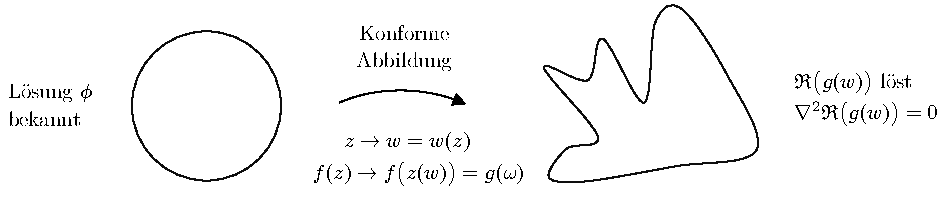
\includegraphics{complex_problems_conformal_map.pdf}
	\caption{Für Probleme mit komplexen Geometrien kann mithilfe einer konformen Abbildung $z$ die Lösung aus der Lösung für den kugelsymmetrischen Fall abgeleitet werden. }
	\label{fig:complex_problems_conformal_map}
\end{figure}

Obwohl die Wahl der Kugelkoordinaten nur für wenige Probleme sinnvoll ist, kann die Lösung für das kugelförmige Problem durch konforme Abbildungen auf komplexere Geometrien angewandt werden (\Abbref{fig:complex_problems_conformal_map}).

\section{Multipolentwicklung}

Bei der Multipolentwicklung klassifiziert man bestimmte Ladungsverteilungen nach sogenannten Momenten (Dipolmoment, Quadrupolmoment, {\ldots}). Zum Beispiel beschreibt das Dipolmoment zwei räumlich voneinander getrennte Ladungen unterschiedlichen Vorzeichens. Auch ein nach außen insgesamt elektrisch neutraler Körper kann ein Dipolmoment aufweisen, nämlich wenn die Schwerpunkte von der positiven und negativen Ladung nicht zusammenfallen. Ein prominentes mikroskopisches Beispiel ist das Wassermolekül (\Abbref{fig:water_molecule}), bei dem das Sauerstoffatom eine bedeutend größere Elektronegativität besitzt als die Wasserstoffatome und dadurch eine Ladungsverschiebung der gebundenen Elektronen zum Sauerstoffatom hin bewirkt. Dadurch besitzt dieses lokal eine Ladung von $\SI{-0.8}{\eV}$, während die Wasserstoffatome eine Ladung von je $\SI{+0.4}{\eV}$ tragen.

Das Dipolmoment $\vec {p}$ ist ein Vektor und per Definition von der negativen Ladung zur positiven gerichtet. Die Einheit des Dipolmoments ist $\SI{1}{Debye}=\SI{3,34e-30}{\coulomb\m}$.



\begin{figure}[htb]
	\centering
	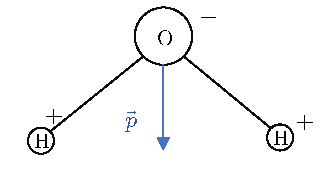
\includegraphics{water_molecule.pdf}
	\caption{Das Wassermolekül ist ein Dipol, bei dem das Sauerstoffatom eine negative Partialladung trägt, während die Wasserstoffatome aufgrund ihrer geringeren Elektronegativität entsprechend positiv geladen sind. }
	\label{fig:water_molecule}
\end{figure}

Für die Multipolentwicklung wird das Potential
\begin{equation*}
	\phi \left(\vec {r}\right)=\frac{1}{4\pi \varepsilon _{0}}\int \diff ^{3}\vec {r}'\frac{\rho \left(\vec {r}\right)}{\left| \vec {r}-\vec {r}'\right| }
\end{equation*}
nach den sogenannten Momenten der Ladungsverteilung entwickelt. Führe dazu zunächst eine Taylorentwicklung für den Ausdruck $1/\left| \vec {r}-\vec {r}'\right| $ um $\vec {r}$ durch ($\left| \vec {r}\right| =r$, Einsteinsche Summenkonvention):
\begin{equation*}
	\frac{1}{\left| \vec {r}-\vec {r}'\right| }=\frac{1}{r}-x_{i}'\partial _{i}\frac{1}{r}+\frac{1}{2}x_{i}'x_{j}'\partial _{i}\partial _{j}\frac{1}{r}+\ldots +\frac{\left(-1\right)^{n}}{n!}x_{i_{1}}'\ldots x_{i_{n}}'\partial _{{i_{1}}}\ldots \partial _{{i_{n}}}\frac{1}{r}
\end{equation*}
Damit lässt sich das Potential nähern als
\begin{align*}
	\phi \left(\vec {r}\right)&\approx \frac{1}{4\pi \varepsilon _{0}}\left(\int \diff ^{3}\vec {r}'\frac{\rho \left(\vec {r}\right)}{r}-\int \diff ^{3}\vec {r}'\rho \left(\vec {r}\right)x_{i}'\partial _{i}\frac{1}{r}+\frac{1}{2}\int \diff ^{3}\vec {r}'\rho \left(\vec {r}\right)x_{i}'x_{j}'\partial _{i}\partial _{j}\frac{1}{r}+\ldots \right. \\ &\quad\quad\left. +\frac{\left(-1\right)^{n}}{n!}\int \diff ^{3}\vec {r}'\rho \left(\vec {r}\right)x_{i_{1}}'\ldots  x_{i_{n}}'\partial _{{i_{1}}}\ldots \partial _{{i_{n}}}\frac{1}{r}\right)\\&=\frac{1}{4\pi \varepsilon _{0}}\left(\frac{1}{r}\underset{q}{\underbrace{\int \diff ^{3}\vec {r}'\rho \left(\vec {r}\right)}}-\partial _{i}\frac{1}{r}\underset{p_{i}}{\underbrace{\int \diff ^{3}\vec {r}'\rho \left(\vec {r}\right)x_{i}'}}+\frac{1}{6}\partial _{i}\partial _{j}\frac{1}{r}\underset{Q_{ij}}{\underbrace{\int \diff ^{3}\vec {r}'\rho \left(\vec {r}\right)\left(3x_{i}'x_{j}'-r^{'2}\delta _{ij}\right)}}+\ldots \right. \\ &\quad\quad\left.  +\,\partial _{{i_{1}}}\ldots \partial _{{i_{n}}}\frac{1}{r}\underset{M_{{i_{1}}\ldots {i_{n}}}}{\underbrace{\frac{\left(-1\right)^{n}}{n!}\int \diff ^{3}\vec {r}'\rho \left(\vec {r}\right)x_{i_{1}}'\ldots x_{i_{n}}'}}\right)\\&=\frac{1}{4\pi \varepsilon _{0}}\left(\frac{q}{r}-p_{i}\partial _{i}\frac{1}{r}+\frac{1}{6}Q_{ij}\partial _{i}\partial _{j}\frac{1}{r}+\ldots +M_{{i_{1}}\ldots {i_{n}}}\partial _{{i_{1}}}\ldots \partial _{{i_{n}}}\frac{1}{r}\right).
\end{align*}
Dabei identifizieren wir das Dipolmoment als Tensor erster Stufe
\begin{equation*}
	p_{i}=\int \diff ^{3}\vec {r}'\rho \left(\vec {r}\right)x_{i}',
\end{equation*}
das Quadrupolmoment als Tensor zweiter Stufe
\begin{equation*}
	Q_{ij}=\int \diff ^{3}\vec {r}'\left(3x_{i}'x_{j}'-r^{'2}\delta _{ij}\right)\rho \left(\vec {r}\right),
\end{equation*}
bei dem standardmäßig noch der Term $-r^{'2}\delta _{ij}$ hinzugefügt wird, welcher aber nicht zu $\phi(\vec r) $ beiträgt, weil
\begin{equation*}
	\delta _{ij}\partial _{i}\partial _{j}\frac{1}{r}=\sum _{i}\partial _{i}^{2}\frac{1}{r}=\nabla ^{2}\frac{1}{r}=0
\end{equation*}
und schließlich das $n$-te Multipolmoment
\begin{equation*}
	M_{{i_{1}}\ldots {i_{n}}}\propto \int \diff ^{3}\vec {r}'\rho \left(\vec {r}\right)x_{i_{1}}'\ldots x_{i_{n}}'.
\end{equation*}
Mit den Identitäten
\begin{equation*}
	\partial _{i}\frac{1}{r}=-\frac{1}{r^{2}}\partial _{i}r=-\frac{x_{i}}{r^{3}},\quad \partial _{i}\partial _{j}\frac{1}{r}=\frac{3x_{i}x_{j}}{r^{5}}-\frac{\delta _{ij}}{r^{3}},
\end{equation*}
(wobei der Term $\delta_{ij}/r^3$ irrelevant ist wegen $\delta _{ij}Q_{ij}=Q_{ii}=0$) erhält man dann für das Potential
\begin{equation*}
	\phi \left(\vec {r}\right)=\frac{1}{4\pi \varepsilon _{0}}\left(\frac{q}{r}+\frac{\vec {p}\cdot \vec {r}}{r^{3}}+\frac{1}{2}Q_{ij}\frac{x_{i}x_{j}}{r^{5}}+\ldots \right).
\end{equation*}



\subsection{Diskussion der Multipolmomente}

\begin{enumerate}
	\item Monopol (Potential/Feld einer Punktladung $\rho _{m}=q\delta \left(\vec {r}\right)$)
		\begin{equation*}
			\phi _{\mathrm{m}}\left(\vec {r}\right)=\frac{1}{4\pi \varepsilon _{0}}\frac{q}{r}\rightarrow \vec {E}(\vec r)=\frac{q}{4\pi \varepsilon _{0}}\frac{\vec {r}}{r^{3}}
		\end{equation*}
	\item Dipol:
		\begin{align*}
				\phi _{\diff }&=-\frac{1}{4\pi \varepsilon _{0}}\vec {p}\cdot \nabla \frac{1}{r}=\frac{1}{4\pi \varepsilon _{0}}\frac{\vec {p}\cdot \vec {r}}{r^{3}}\propto \frac{1}{r^{2}} \\
				E_{i}&=\frac{1}{4\pi \varepsilon _{0}}p_{j}\nabla _{i}\nabla _{j}\frac{1}{r}=\frac{1}{4\pi \varepsilon _{0}}\frac{p_{j}}{r^{3}}\left(\frac{3x_{i}x_{j}}{r^{2}}-\delta _{ij}\right)\propto \frac{1}{r^{3}}
		\end{align*}
		Wir sehen, dass das Feld eines Dipols mit $r^{-3}$ abnimmt, während dasjenige eines Monopols nur mit $r^{-2}$ abfällt. Die Felder der einzelnen Ladungen heben sich im Fernfeld zum Teil auf.

		Die Ladungsdichte eines elementaren Dipols ist
		\begin{equation*}
			\rho _{\diff }\left(\vec {r}\right)=q\left(\delta \left(\vec {r}-\frac{\vec {d}}{2}\right)-\delta \left(\vec {r}+\frac{\vec {d}}{2}\right)\right),
		\end{equation*}
		woraus sich ein Dipolmoment von
		\begin{equation*}
			\vec {p}=q\vec {d}\parallel \vec {d}
		\end{equation*}
		ergibt. 

		Man kann auch einen sogenannten Punktdipol betrachten \textendash{} ein idealisiertes Objekt, bei dem der Abstand $\vec {d}$ gegen $0$ geht:
		\begin{equation*}
			\vec {p}=\lim _{\substack{
					d\rightarrow 0 \\
					qd<\infty}} q\vec {d},\quad \rho _{\diff }\left(\vec {r}\right)=-\vec {p}\cdot \nabla \delta \left(\vec {r}\right), \quad\phi _{\diff }=-\frac{1}{4\pi \varepsilon _{0}}\vec {p}\cdot \nabla \frac{1}{r}
		\end{equation*}
	\item Quadrupol:
		\begin{align*}
				\phi _{\mathrm{Q}}&=\frac{1}{4\pi \varepsilon _{0}}\frac{1}{6}Q_{kl}\nabla _{k}\nabla _{l}\frac{1}{r}=\frac{1}{4\pi \varepsilon _{0}}\frac{1}{2}Q_{kl}\frac{x_{k}x_{l}}{r^{5}}\propto \frac{1}{r^{3}} \\
				E_{i}&=-\frac{1}{4\pi \varepsilon _{0}}\frac{1}{6}Q_{kl}\nabla _{i}\nabla _{k}\nabla _{l}\frac{1}{r}=\frac{1}{4\pi \varepsilon _{0}}\frac{Q_{kl}}{2}\frac{5x_{i}x_{k}x_{l}-r^{2}\left(\delta _{kl}x_{i}+\delta _{il}x_{k}+\delta _{ik}x_{l}\right)}{r^{7}}
		\end{align*}


		\begin{figure}[htb]
			\centering
			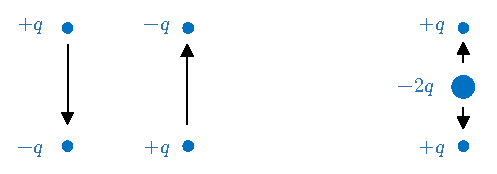
\includegraphics{elemental_quadrupoles.pdf}
			\caption{Elementare Quadrupole können in zwei verschiedenen Konfigurationen auftreten. }
			\label{fig:elemental_quadrupoles}
		\end{figure}

		Es gibt zwei elementare Quadrupole (mit $\vec {p}=0$), die in \Abbref{fig:elemental_quadrupoles} zu sehen sind. 

		Wird der Bezugspunkt/Aufpunkt verschoben, so ändern sich im Allgemeinen die Multipolmomente, aber das erste Moment, das bei der Multipolentwicklung einer Ladungsverteilung ungleich $0$ ist, bleibt unverändert.


		\begin{formal}
			Das niedrigste, nicht-verschwindende Multipolmoment in der Entwicklung ist unabhängig vom Bezugspunkt.
		\end{formal}
		Man kann auch sphärische Multipolmomente mithilfe von Kugelflächenfunktionen ausdrücken.
\end{enumerate}


\subsection{Energie von Multipolen im äußeren Feld}

Die Energie von Multipolen in einem externen Potential $\phi _{e}\left(\vec {r}\right)$ kann aus der bereits bekannten Formel für die Energie einer beliebigen Ladungsverteilung $\rho \left(\vec {r}\right)$ abgeleitet werden,
\begin{equation*}
	U=\int _{V}\diff ^{3}\vec {r}\rho \left(\vec {r}\right)\phi _{e}\left(\vec {r}\right).
\end{equation*}
Wir nehmen an, dass die Änderung von $\phi _{e}$ in $V$ nur klein ist und erhalten durch eine Taylor-Entwicklung
\begin{align*}
	U&=\int \diff ^{3}\vec {r}\rho \left(\vec {r}\right)\left[\phi _{e}\left(0\right)+\vec {r}\nabla \phi _{e}\left(0\right)+\frac{1}{2}x_{i}x_{j}\nabla _{i}\nabla _{j}\phi _{e}\left(0\right)+\ldots \right]\\&=q\phi \left(0\right)-\vec {p}\cdot E_{e}\left(0\right)-\frac{1}{6}Q_{ij}\nabla _{j}E_{e}^{\left(i\right)}\left(0\right)+\ldots
\end{align*}
Die Energie der Multipole ist also durch die $n$-fache Ableitung des Potentials $\nabla ^{n}\phi $ bestimmt. Diese Rechnung erlaubt wegen der Taylor-Entwicklung eine beliebige Wahl des Bezugspunkts.

\begin{figure}[htb]
	\centering
	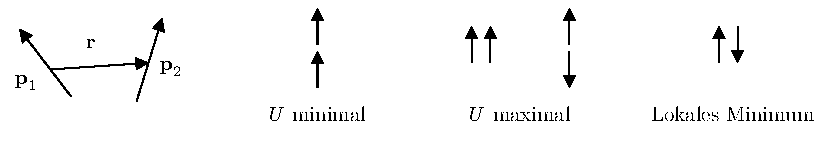
\includegraphics{dipoles.pdf}
	\caption{Links: Schematische Darstellung zweier Dipole $\vec p_1$, $\vec p_2$ mit Abstand $\vec r$. Weitere Abbildungen: Spezielle Anordnungen zweier Dipole, für die die Energie extremal wird. }
	\label{fig:dipoles}
\end{figure}

Als typisches Beispiel soll die Wechselwirkung zweier Dipole betrachtet werden. Die potentielle Energie kann berechnet werden, indem der Dipol $\vec {p}_{2}$ wie oben beschrieben in das Feld des Dipols $\vec {p}_{1}$ gesetzt wird (oder umgekehrt):
\begin{equation*}
	U_{\mathrm{DD}}=-\vec {p}_{2}\cdot \vec {E}_{1}\left(\vec {r}\right)=-\frac{1}{4\pi \varepsilon _{0}}\frac{1}{r^{3}}\left(\frac{3\left(\vec {r}\cdot \vec {p}_{1}\right)\left(\vec {r}\cdot \vec {p}_{2}\right)}{r^{2}}-\vec {p}_{1}\cdot \vec {p}_{2}\right)
\end{equation*}
Diese wird minimal für $\vec {p}_{1}\parallel \vec {p}_{2}\parallel \vec {r}$ und maximal für $\vec {p}_{1}\parallel \vec {p}_{2}\perp \vec {r}$. Diese Konfigurationen sind in \Abbref{fig:dipoles} zusammengestellt. Für antiparallele $\vec {p}_{1}$ und $\vec {p}_{2}$ und $\vec {p}_{1},\vec {p}_{2}\perp \vec {r}$ wird außerdem ein lokales Minimum erreicht. Aus diesem Grund bilden Dipolmoleküle auch häufig Molekülketten.

Zuletzt sollen noch Drehmomente auf Multipole diskutiert werden.
\begin{align*}
		\vec {M}          & =\int \diff ^{3}\vec {r}\vec {r}\times \underset{\text{Kraftdichte}}{\underbrace{\rho \left(\vec {r}\right)\vec {E}_{e}\left(\vec {r}\right)}}\implication M_{i}=\int \diff ^{3}\vec {r}\varepsilon _{ijk}x_{j}\rho \left(\vec {r}\right)\underset{\approx E_{e}^{\left(k\right)}\left(0\right)+x_{l}\nabla _{l}E_{e}^{\left(k\right)}\left(0\right)}{\underbrace{E_{e}^{\left(k\right)}\left(\vec {r}\right)}} \\
		\implication M_{i} & =\left(\vec {p}\times \vec {E}_{e}\right)_{i}+\frac{1}{3}\varepsilon _{ijk}Q_{jl}\nabla _{l}E_{e}^{\left(k\right)}
\end{align*}
Insbesondere dreht das Drehmoment $\vec {M}$ einen Dipol parallel zu $\vec {E}$, da $\vec {M}=0$ für $\vec {p}\parallel \vec {E}_{e}$ und
\begin{equation*}
	U=-\vec {p}\cdot \vec {E}_{e}=-pE_{e}\cos \vartheta \implication M=-\frac{\partial U}{\partial \vartheta }=-pE_{e}\sin \vartheta =-\left| \vec {p}\times \vec {E}_{e}\right| .
\end{equation*}
% !TEX root = Theo_III.tex


\chapter{Elektrische Felder in Materie}

In diesem Kapitel werden die makroskopischen Gleichungen der Elektrostatik in Materie beschrieben und erläutert.



\section{Mikroskopische Gleichungen der Elektrostatik und Mittelung\label{sec:mikroskopische_gleichungen_der_elektrostatik}}

Bis jetzt haben wir nur freie Ladungen betrachtet. Die Ladungsdichte $\rho \left(\vec {r}\right)$ erzeugt ein elektrisches Feld $\vec {E}(\vec r)$. In Materie sind zusätzlich auch gebundene Ladungen vorhanden, die mit dem Feld wechselwirken. Das können (nach außen hin elektrisch neutrale) Atome, geladenen Ionen, permanente Dipole (oder Multipole) sein (z.B. $\mathrm{H}_{2}\mathrm{O}$), sowie Dipole sein, die durch ein äußeres elektrisches Feld induziert werden.

Um diese Wechselwirkung zu beschreiben, wird eine Mittelung der mikroskopischen Gleichungen
\begin{equation*}
	\divg \vec {e}=\frac{1}{\varepsilon _{0}}\rho \left(\vec {r}\right),\quad \rot \vec {e}=0
\end{equation*}
durchgeführt. Wir haben bisher einzelne Ladungen durch $\delta $-Funktionen in der Ladungsdichte beschrieben. Dadurch kommt es zu starken räumlichen Ladungsschwankungen. Für eine makroskopische Betrachtung in Größenordnungen von Nanometern wenden wir eine räumliche Mittelung bzw. Glättungsfunktion auf die Ladungsdichteverteilung an.




\subsection{Glättungsfunktion}

Um eine stark variierende Funktion $F\left(\vec {r},t\right)$ zu mitteln, wird sie mit einer sogenannten Glättungsfunktion $f$ gefaltet. Dabei kann es sich z.B. um eine Gauß-Funktion handeln:
\begin{equation*}
	F\left(\vec {r},t\right) \xrightarrow{\text{Mittelung}} \left\langle F\left(\vec {r},t\right)\right\rangle =\int f\left(\left| \vec {r}-\vec {r}'\right| \right)F\left(\vec {r}',t\right)\diffa[3]{\vec{r}'}
\end{equation*}
Für eine Punktladung $F\left(\vec {r}\right)=F_{0}\delta \left(\vec {r}-\vec {r}_{0}\right)$ ist dann zum Beispiel $\left\langle F\right\rangle =F_{0}f\left(\vec {r}-\vec {r}_{0}\right)$.

Für die Mittelung gelten die folgenden Eigenschaften:\begin{enumerate}
	\item Die Mittelung der konstanten Funktion $F=1$ ist genau dann konstant $1$, wenn die Glättungsfunktion über den gesamten Raum auf $1$ normiert ist,
	      \begin{equation*}
		      \left\langle 1\right\rangle =1\equivalence \int \diffa[3]{\vec{r}}f=1.
	      \end{equation*}
	\item $\partial _{i}\left\langle F\right\rangle =\left\langle \partial _{i}F\right\rangle $.
\end{enumerate}



\section{Makroskopische Gleichungen der Elektrostatik\label{sec:Makroskopische_Gleichungen_der_Elektrostatik}}

Mithilfe der Glättung kann man das makroskopische $\vec {E}$-Feld als
\begin{equation*}
	\vec {E}\left(\vec {r},t\right)=\left\langle \vec {e}\left(\vec {r},t\right)\right\rangle
\end{equation*}
schreiben. Für die Ladungsdichte erhält man
\begin{equation*}
	\left\langle \rho \left(\vec {r}\right)\right\rangle =\left\langle \rho _{f}\left(\vec {r}\right)+\rho _{b}\left(\vec {r}\right)\right\rangle =\left\langle \rho _{f}\left(\vec {r}\right)\right\rangle +\left\langle \rho _{b}\left(\vec {r}\right)\right\rangle \equiv \rho _{F}+\rho _{B}.
\end{equation*}
Die gebundenen Ladungen werden als Summe der Ladungsdichten einzelner Moleküle geschrieben:
\begin{equation*}
	\rho _{b}\left(\vec {r}\right)=\sum _{n}\rho _{n}\left(\vec {r}\right), \rho _{n}\left(\vec {r}\right)=\sum _{i}q_{i}\delta \left(\vec {r}-\vec {r}_{i}\right)=\sum _{i}q_{i}\delta \left(\vec {r}-\left(\vec {r}_{n}+\vec {r}_{ni}\right)\right)
\end{equation*}
mit neuen Bezugspunkten $\vec {r}_{n}$ für die einzelnen Moleküle. Für die Mittelung wird dann eine Taylor-Entwicklung um diese neuen Bezugspunkte $\vec {r}_{n}$ durchgeführt:
\begin{align*}
	\left\langle \rho _{n}\left(\vec {r}\right)\right\rangle & =\sum _{i}q_{i}f\left(\vec {r}-\left(\vec {r}_{n}+\vec {r}_{ni}\right)\right) \\&=\sum _{i}q_{i}\left[f\left(\vec {r}-\vec {r}_{n}\right)-\vec {r}_{ni}\cdot \nabla f\left(\vec {r}-\vec {r}_{n}\right)+\frac{1}{2}\left(\vec {r}_{ni}\right)_{k}\left(\vec {r}_{ni}\right)_{l}\nabla _{k}\nabla _{l}f\left(\vec {r}-\vec {r}_{n}\right)+\ldots \right]
\end{align*}
Daraus können die molekularen Dipolmomente bestimmt werden:
\begin{align*}
	q_{n}                            & =\sum _{i}q_{i}                                                              & \text{(Molekulare Ladung)}           \\
	\vec {p}_{n}                     & =\sum _{i}q_{i}\vec {r}_{ni}                                                 & \text{(Molekulares Dipolmoment)}     \\
	\left(\mathrm{Q}_{n}\right)_{kl} & =3\sum _{i}q_{i}\left(\vec {r}_{ni}\right)_{k}\left(\vec {r}_{ni}\right)_{l} & \text{(Molekulares Quadrupolmoment)}
\end{align*}
(vgl. Multipolmomente einer kontinuierlichen Ladungsverteilung, aber hier jetzt diskret). Insgesamt ergibt sich eine Verschmierung punktförmiger molekularer Multipole:
\begin{align*}
	\left\langle \rho _{n}\left(\vec {r}\right)\right\rangle & =q_{n}f\left(\vec {r}-\vec {r}_{n}\right)-\vec {p}_{n}\cdot \nabla f\left(\vec {r}-\vec {r}_{n}\right)+\frac{1}{6}\left(\mathrm{Q}_{n}\right)_{kl}\nabla _{k}\nabla _{l}f\left(\vec {r}-\vec {r}_{n}\right) \\&=\left\langle q_{n}\delta \left(\vec {r}-\vec {r}_{n}\right)\right\rangle -\nabla \cdot \left\langle p_{n}\delta \left(\vec {r}-\vec {r}_{n}\right)\right\rangle +\frac{1}{6}\nabla _{k}\nabla _{l}\left\langle \left(\mathrm{Q}_{n}\right)_{kl}\delta \left(\vec {r}-\vec {r}_{n}\right)\right\rangle
\end{align*}
und für die gemittelte gebundene Ladungsdichte:
\begin{equation*}
	\left\langle \rho _{b}\left(\vec {r}\right)\right\rangle =\rho _{\mathrm{m}}\left(\vec {r}\right)-\nabla \cdot \vec {P}\left(\vec {r}\right)+\nabla _{k}\nabla _{l}{Q}_{\mathrm{kl}}+\ldots
\end{equation*}
mit der makroskopischen Ladungsdichte (Monopoldichte)
\begin{equation*}
	\rho _{\mathrm{m}}\left(\vec {r}\right)=\left\langle \sum _{n}q_{n}\delta \left(\vec {r}-\vec {r}_{n}\right)\right\rangle ,
\end{equation*}
der Polarisation (Dipolmomentdichte)
\begin{equation*}
	\vec {P}\left(\vec {r}\right)=\left\langle \sum _{n}\vec {p}_{n}\delta \left(\vec {r}-\vec {r}_{n}\right)\right\rangle
\end{equation*}
und so weiter.


Damit ergibt sich jetzt insgesamt die gemittelte mikroskopische Ladungsdichte
\begin{equation*}
	\left\langle \rho \left(\vec {r}\right)\right\rangle =\left\langle \rho _{f}\left(\vec {r}\right)\right\rangle +\left\langle \rho _{b}\left(\vec {r}\right)\right\rangle =\underset{\rho _{\mathrm{Ma}}\left(\vec {r}\right)}{\underbrace{\rho _{F}\left(\vec {r}\right)+\rho _{m}\left(\vec {r}\right)}}\underset{\rho _{\mathrm{Mi}}\left(\vec {r}\right)}{\underbrace{-\nabla \cdot \vec {P}\left(\vec {r}\right)+\nabla _{k}\nabla _{l}Q_{kl}\left(\vec {r}\right)}}
\end{equation*}
und es folgt für die makroskopischen Feldgleichungen
\begin{align*}
	\left\langle \divg \vec {e}\right\rangle & =\frac{1}{\varepsilon _{0}}\left\langle \rho \left(\vec {r}\right)\right\rangle ,\quad \left\langle \rot \vec {e}\right\rangle =\vec {0}                                                                                                                                                               \\
	\divg \vec {E}                           & =\frac{1}{\varepsilon _{0}}\left(\rho _{\mathrm{Ma}}\left(\vec {r}\right)+\rho _{\mathrm{Mi}}\left(\vec {r}\right)\right)=\frac{1}{\varepsilon _{0}}\left(\rho _{\mathrm{Ma}}\left(\vec {r}\right)-\nabla \cdot \vec {P}\left(\vec {r}\right)+\nabla _{k}\nabla _{l}Q_{kl}\left(\vec {r}\right)\right)
\end{align*}
und
\begin{equation*}
	\rot \vec {E}=\vec {0}.
\end{equation*}
An dieser Stelle führen wir jetzt das sogenannte dielektrische Verschiebungsfeld $\vec {D}$ ein:
\begin{equation*}
	\vec {D}\left(\vec {r}\right)=\varepsilon _{0}\vec {E}\left(\vec {r}\right)+\vec {P}\left(\vec {r}\right)-\nabla Q\left(\vec {r}\right)
\end{equation*}
Dabei ist die Idee, dass höhere Multipole der Ladungen jetzt in dem Hilfsfeld $\vec {D}$ stecken. In der Regel wird übrigens bereits das Quadrupolmoment vernachlässigt.

Damit können die makroskopischen Feldgleichungen jetzt geschrieben werden als
\begin{equation*}
	\boxed{\divg \vec {D}=\rho _{\mathrm{Ma}}\left(\vec {r}\right), \quad\rot \vec {E}=0.}
\end{equation*}
Die Quellen des dielektrischen Verschiebungsfeldes sind also die makroskopischen Ladungsdichten und nicht die höheren Multipolmomente. Außerdem ist $\vec {D}$ nur ein Hilfsfeld, das fundamentale Feld ist das elektrische Feld $\vec {E}$.

Die Polarisation $\vec {P}$ wird zur Darstellung in der Regel nach $\vec {E}$ entwickelt,
\begin{equation*}
	P_{i}\left(\vec {E}\right)=\varepsilon _{0}\chi _{ij}^{\left(1\right)}E_{j}+\varepsilon _{0}\chi _{ijk}^{\left(2\right)}E_{j}E_{k}+\ldots ,
\end{equation*}
wobei $\chi _{ij}^{\left(1\right)}, \chi _{ijk}^{\left(2\right)},\ldots $ die hier neu eingeführten elektrischen Suszeptibilitätstensoren sind. Im linearen, isotropen Medium gilt
\begin{equation*}
	\vec {P}\left(\vec {E}\right)=\varepsilon _{0}\chi \vec {E},
\end{equation*}
wobei $\chi $ ein Skalar ist. Das trifft hauptsächlich auf Gase, Flüssigkeiten und kubischen Kristalle zu. In anisotropen Medien ist $\chi ^{\left(1\right)}$ ein Tensor zweiter Stufe und für nicht-lineare Medien werden noch höhere Suszeptibilitäten $\chi ^{\left(n\right)}$ relevant, die Tensoren der Stufe $\left(n+1\right)$ sind. Diese sind besonders wichtig in der nicht-linearen Optik. Im Allgemeinen ist die Polarisation nicht parallel zum elektrischen Feld und nur im linearen und isotropen Fall ist $\vec {P}\parallel \vec {E}$.

Häufig wird auch der dielektrische Tensor $\varepsilon $ eingeführt:
\begin{equation*}
	\vec {D}\left(\vec {r}\right)=\varepsilon _{0}\vec {E}\left(\vec {r}\right)+\vec {P}\left(\vec {r}\right)\equiv \varepsilon \vec {E}\left(\vec {r}\right), \quad\varepsilon \equiv \varepsilon _{0}\left(1+\chi ^{\left(1\right)}\right)
\end{equation*}
Dieser ist uns für den linearen, isotropen Fall wiederum schon bekannt als Dielektrizitätskonstante oder Permittivität $\varepsilon _{r}=\chi +1$.

Eine andere Beschreibung erfolgt mithilfe der atomaren Polarisierbarkeit $\alpha $ (im Allgemeinen ebenfalls ein Tensor zweiter Stufe), die das molekulare Dipolmoment mit dem elektrischen Feld verbindet,
\begin{equation*}
	\vec {p}=\varepsilon _{0}\alpha \vec {E}.
\end{equation*}
Mit der Dipoldichte $n=N/V$ lässt sich die Polarisation schreiben als
\begin{equation*}
	\vec {P}=\varepsilon _{0}n\alpha \vec {E}, \quad\chi ^{\left(1\right)}=n\alpha .
\end{equation*}
Polarisation kann in einem Medium auftreten als permanente, ausgerichtete Dipole (in ferroelektrischen Materialien), die durch die Kristallstruktur bedingt sind, als induzierte Polarisation durch Ausrichtung von ungeordneten permanenten Dipolen gegen die thermische Bewegung oder durch Verschiebung von Ladungen innerhalb des Mediums (typisch für Dielektrika).



\section{Randbedingungen von Dielektrika und Anwendungen\label{sec:randbedingungen_von_dielektrika}}



\subsection{Randbedingungen und Polarisationsladung}

Die Randbedingungen bei Übergängen zwischen zwei Medien lassen sich ähnlich herleiten wie in Kapitel \ref{sec:randbedingungen_auf_grenzflaechen}. Betrachte zunächst die Tangentialkomponente des elektrischen Feldes, wie in \Abbref{fig:bc_dielectrica} dargestellt. Da $\rot \vec {E}=\vec {0}$, erhält man die folgende Randbedingung für die Tangentialkomponente:
\begin{equation*}
	\hat{\vec {t}}\cdot \left(\vec {E}^{\left(2\right)}-\vec {E}^{\left(1\right)}\right)=0\equivalence \vec {E}_{\parallel }^{\left(1\right)}=\vec {E}_{\parallel }^{\left(2\right)}
\end{equation*}


\begin{figure}[htb]
	\centering
	\tFigRandbedingungenDielektrikum
	\caption{Übergang zwischen zwei Dielektrika. Die Felder $\vec E$, $\vec D$ und $\vec P$ ändern sich auf der Grenzfläche, an welcher sich eine Flächenladungsdichte $\sigma$ ausbildet. }
	\label{fig:bc_dielectrica}
\end{figure}

Für die Normalkomponente von $\vec {D}$ folgt aus $\divg \vec {D}=\rho _{\mathrm{Ma}}$
\begin{equation*}
	\hat{\vec {n}}\cdot \left(\vec {D}^{\left(2\right)}-\vec {D}^{\left(1\right)}\right)=D_{\perp }^{\left(2\right)}-D_{\perp }^{\left(1\right)}=\sigma
\end{equation*}
mit makroskopischer Flächenladungsdichte $\sigma $ auf der Grenzfläche\footnote{Für lineare, isotrope Dielektrika gilt insbesondere $\varepsilon _{2}E_{\perp }^{\left(2\right)}=\varepsilon _{1}E_{\perp }^{\left(1\right)}+\sigma .$}. Dieser Zusammenhang lässt sich mithilfe von $D_{\perp }^{\left(i\right)}=\varepsilon _{0}E_{\perp }^{\left(i\right)}+P_{\perp }^{\left(i\right)}$ auch kombiniert über das elektrische Feld und die Polarisation ausdrücken als
\begin{equation*}
	E_{\perp }^{\left(2\right)}-E_{\perp }^{\left(1\right)}=\frac{1}{\varepsilon _{0}}\left(\sigma +P_{\perp }^{\left(1\right)}-P_{\perp }^{\left(2\right)}\right).
\end{equation*}
Für den Spezialfall $\sigma =0$ wird in
\begin{align*}
	E_{\perp }^{\left(2\right)}-E_{\perp }^{\left(1\right)}=\frac{1}{\varepsilon _{0}}\left(P_{\perp }^{\left(1\right)}-P_{\perp }^{\left(2\right)}\right)\equiv \frac{1}{\varepsilon _{0}}\sigma _{p}
\end{align*}
die Polarisationsladung $\sigma _{p}$ definiert. Es gibt also aufgrund des Sprungs der Polarisation auf der Grenzfläche einen Sprung der Normalkomponente $E_{\perp }$. Das führt auf ein Brechungsgesetz (\Abbref{fig:dielectric_refraction}):

\begin{formal}
	Beim Übergang zum dielektrisch dünneren Medium wird das elektrische und das dielektrische Feld zum Lot hin gebrochen.
\end{formal}



\begin{figure}[htb]
	\centering
	\tfigDielektrischeBrechung
	\caption{Die elektrischen Felder werden beim Übergang in Medien mit anderer Permittivität gebrochen, ähnlich zu der optischen Brechung. }
	\label{fig:dielectric_refraction}
\end{figure}

Diese Brechung ist ganz ähnlich zur optischen Brechung (wenn auch genau umgekehrt, denn dort wird das Licht beim Übergang in das optisch dichtere Medium zum Lot hin gebrochen). Es gilt
\begin{equation*}
	\vec {E}_{\parallel }^{\left(1\right)}=\vec {E}_{\parallel }^{\left(2\right)},\quad E_{\perp }^{\left(2\right)}=\frac{\varepsilon _{1}}{\varepsilon _{2}}E_{\perp }^{\left(1\right)}.
\end{equation*}
Diese Randbedingungen ermöglichen auch eine Messung von $\vec {D}$ und $\vec {E}$, indem eine Probeladung in einen schmalen Spalt im zu vermessenden Dielektrikum eingebracht wird, wie in \Abbref{fig:measure_fields_in_dielectricum} zu sehen.

\begin{figure}[htb]
	\centering
	\tfigMessungVonFeldDurchRandbedingungen
	\caption{Indem eine Probeladung in einem schmalen Spalt in ein Dielektrikum gebracht wird, können mithilfe der Randbedingungen die elektrischen Felder in diesem gemessen werden. Wird der Spalt senkrecht zu den Feldlinien gesetzt, so erfährt die Probeladung gerade die Kraft, die aus dem äußeren Feld $\vec E_0=\vec D/\varepsilon_0$ resultiert, was eine Messung der dielektrischen Verschiebung $\vec D$ ermöglicht. Bei einer parallelen Ausrichtung spürt die Ladung nur das Feld $\vec E_0=\vec E$. }
	\label{fig:measure_fields_in_dielectricum}
\end{figure}




\subsection{Entelektrisierungsfelder}


\begin{figure}[htb]
	\centering
	\tfigDielektrischeKugelHomogenesEFeld
	\caption{Eine dielektrische Kugel in einem ursprünglich homogenen äußeren Feld $\vec E_0=E_0 \vec e_z$ beeinflusst die Feldlinien, weil die Randbedingungen erfüllt werden müssen. Innerhalb der Kugel ist das Feld homogen. }
	\label{fig:dielectric_sphere_in_homogeneous_field}
\end{figure}

Wird ein Dielektrikum einem äußeren elektrischen Feld $\vec {E}_{0}$ ausgesetzt, erzeugt die Polarisation ein sogenanntes Entelektrisierungs- oder Polarisationsfeld, welches das äußere Feld abschwächt. Der Grund sind Oberflächenladungen durch Polarisation.

Das Entelektrisierungsfeld soll exemplarisch für eine dielektrische Kugel in einem homogenen äußeren Feld berechnet werden (\Abbref{fig:dielectric_sphere_in_homogeneous_field}).

Da es keine freien Ladungen gibt, also $\rho _{\mathrm{Ma}}=0$, ist die Laplace-Gleichung $\nabla ^{2}\phi =0$ zu lösen. Aufgrund der Axialsymmetrie um die $z$-Achse wird als Lösungsansatz eine Linearkombination aus Legendre-Polynomen erster Ordnung für die Beschreibung der Potentiale $\phi _{i}$ innerhalb und $\phi _{a}$ außerhalb der Kugel verwendet:
\begin{equation*}
	\phi _{i,a}=\sum _{l=0}^{\infty }\left(a_{l}^{\left(i,a\right)}r^{l}+b_{l}^{\left(i,a\right)}r^{-\left(l+1\right)}\right)P_{l}\left(\cos \vartheta \right)
\end{equation*}
Aus Betrachtungen für die Grenzfälle können die Koeffizienten $a_{l}^{\left(i,a\right)}$ und $b_{l}^{\left(i,a\right)}$ ermittelt werden:

\begin{enumerate}[i)]
	\item Im Unendlichen ($r\rightarrow \infty $) verschwindet die Störung durch die dielektrische Kugel und das Feld ist homogen, $E_{0}\vec {e}_{z}=-\nabla \phi _{a}$. Das Potential nimmt dort also die Form $\phi _{a}\left(r\rightarrow \infty \right)=-E_{0}z=-E_{0}r\cos \vartheta $ an. Durch einen Koeffizientenvergleich erhält man $a_{1}^{\left(a\right)}=-E_{0}, a_{l>1}^{\left(a\right)}=0$.

	\item Im Mittelpunkt ($r=0$) darf das Potential nicht divergieren, sodass $b_{l}^{\left(i\right)}=0$ für alle $l$.

	\item An der Grenzfläche ($r=R$) muss gelten, dass $E_{\parallel }^{\left(i\right)}=E_{\parallel }^{\left(a\right)}$ und $\varepsilon _{r}E_{\perp }^{\left(i\right)}=E_{\perp }^{\left(a\right)}$. Einsetzen und Lösen des Gleichungssystems führt auf
	      \begin{equation*}
		      a_{1}^{\left(i\right)}=-\frac{3}{\varepsilon _{r}+2}E_{0},\quad b_{1}^{\left(a\right)}=\frac{\varepsilon _{r}-1}{\varepsilon _{r}+2}R^{3}E_{0},\quad a_{l>1}^{\left(i\right)}=0,\quad b_{l>1}^{\left(a\right)}=0.
	      \end{equation*}
\end{enumerate}

Mit den Ersetzungen $r\cos \vartheta =z=\vec {r}\cdot \vec {e}_{z}$ und dem Dipolmoment $\vec {p}=\frac{4}{3}\pi R^{3}\vec {P}$ erhält man schließlich
\begin{equation*}
	\phi _{i}=-\frac{3}{\varepsilon _{r}+2}\vec {E}_{0}\cdot \vec {r}, \quad\phi _{a}=-\vec {E}_{0}\cdot \vec {r}+\frac{1}{4\pi \varepsilon _{0}}\frac{\vec {p}\cdot \vec {r}}{r^{3}}
\end{equation*}
und
\begin{equation*}
	\vec {E}^{\left(i\right)}=\frac{3}{\varepsilon _{r}+2}\vec {E}_{0}, \quad\vec {E}^{\left(a\right)}=\vec {E}_{0}-\frac{1}{4\pi \varepsilon _{0}}\nabla \frac{\vec {p}\cdot \vec {r}}{r^{3}}.
\end{equation*}
Im Innern der Kugel ist also das elektrische Feld homogen und die (lineare) Polarisation ist
\begin{equation*}
	\vec {P}=\varepsilon _{0}\chi \vec {E}^{\left(i\right)}=3\varepsilon _{0}\frac{\varepsilon _{r}-1}{\varepsilon _{r}+2}\vec {E}_{0}.
\end{equation*}
Das innere Feld lässt sich auch umformulieren zu
\begin{equation*}
	\vec {E}^{\left(i\right)}=\vec {E}_{0}-\frac{1}{3\varepsilon _{0}}\vec {P},
\end{equation*}
also der Summe des ursprünglichen äußeren Feldes und eines abschwächenden Feldes $\vec {E}'\equiv \vec {P}/3\varepsilon _{0}$ \textendash{} dem abschirmenden Entelektrisierungsfeld (\Abbref{fig:dielectric_ball_polarisation_field}).

\begin{figure}[htb]
	\centering
	\tfigEntelektrisierung
	\caption{Entelektrisierungsfeld/Polarisationsfeld einer dielektrischen Kugel in einem homogenen äußeren elektrischen Feld. }
	\label{fig:dielectric_ball_polarisation_field}
\end{figure}


Für den allgemeinen, nicht kugelsymmetrischen Fall sind Entelektrisierungsfeld $\vec {E}'$ und Polarisation nicht parallel. Dann gilt
\begin{equation*}
	\vec {E}'=-\frac{1}{\varepsilon _{0}}\lambda \vec {P}
\end{equation*}


\begin{figure}[htb]
	\centering
	\tfigSimpleDielectricBodiesEntelektrisierungsfeld
	\caption{Enelektrisierungsfaktor bzw. -tensor von speziellen Geometrien: Kugel, Ellipsoid, Platte (Feld orthogonal), Platte (Feld parallel), Zylinder (Feld parallel), Zylinder (Feld orthogonal). }
	\label{fig:simple_dielectric_bodies_polarisation_field}
\end{figure}

mit dem Entelektrisierungstensor $\lambda$. Für die Kugel ist natürlich $\lambda =1/3$, für eine zum äußeren Feld orthogonale Platte dagegen $\lambda =1$ und für eine zum äußeren Feld parallele Platte $\lambda =0$. Für einen langen Zylinder, der orthogonal zum Feld steht ist $\lambda =1/2$ (siehe \Abbref{fig:simple_dielectric_bodies_polarisation_field}).

Für komplexere dielektrische Körper in einem homogenen äußeren Magnetfeld ist $\vec {P}$ nicht homogen.



\subsection{Clausius-Mosotti-Formel}

Im Kapitel \ref{sec:Makroskopische_Gleichungen_der_Elektrostatik} wurde bereits die molekulare Polarisierbarkeit $\alpha $ eingeführt. Diese beschreibt das induzierte Dipolmoment eines Moleküls in Abhängigkeit von dem lokalen elektrischen Feld
\begin{equation*}
	\vec {p}=\varepsilon _{0}\alpha \vec {E}_{\mathrm{loc}}.
\end{equation*}
Die Clausius-Mosotti-Formel beschreibt, wie die molekulare Polarisierbarkeit mit der (makroskopischen) Dielektrizität $\varepsilon _{r}$ zusammenhängt:
\begin{equation*}
	\frac{\varepsilon _{r}-1}{\varepsilon _{r}+2}=\frac{1}{3}n\alpha
\end{equation*}

\begin{figure}[htb]
	\centering
	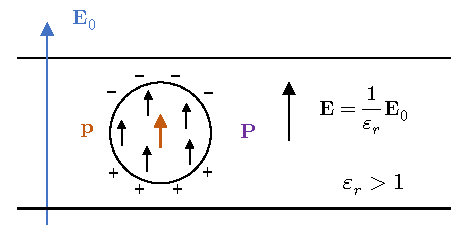
\includegraphics{clausius_mosotti.pdf}
	\caption{Ein Dipol $\vec p$ befindet sich in einem Medium mit $\varepsilon_r >1$. Ein äußeres elektrisches Feld $\vec E_0$ liegt an (lokal homogen). Im Dielektrikum ist die Feldstärke $\vec E=\vec E_0/\varepsilon_r$. Es wird ein kleiner, kugelförmiger Bereich um den Dipol herum betrachtet, innerhalb dessen alle Dipole des Mediums berücksichtigt werden. Der Dipol $\vec p$ ruft eine Polarisation $\vec P$ hervor. }
	\label{fig:clausius_mosotti}
\end{figure}

Die Formel wird hergeleitet aus der in \Abbref{fig:clausius_mosotti} dargestellten Geometrie. Ein äußeres elektrisches Feld $\vec {E}_{0}$ durchdringt das Medium mit $\varepsilon _{r}>1$. Dort ist also das Feld $\vec {E}=\vec {E}_{0}/\varepsilon _{r}$. Im Medium befindet sich ein mikroskopischer Dipol $\vec {p}$. Durch dessen Existenz ist auch eine Polarisation $\vec {P}$ vorhanden, die das Feld innerhalb des Mediums verändert. Um jetzt das lokale Feld beim Dipol zu bestimmen, legen wir eine kleine Hohlkugel um den Dipol herum. Außerhalb dieser Kugel rechnen wir makroskopisch mit der Polarisation, aber innerhalb der Kugel betrachten wir vorsichtshalber die einzelnen Dipole des Dielektrikums (z.B. Dipole auf Gitterplätzen im Festkörper). Der Bereich außerhalb ist also das kontinuierliche Dielektrikum, während innen diskrete Dipole liegen.

Das lokale elektrische Feld hat verschiedene Beiträge: zum einen das Feld $\vec {E}$ im Medium, dann das Feld, das durch die Oberflächenladung (von der Polarisation erzeugt) an der Kugel hervorgerufen wird (sog. Lorentzfeld) und schließlich das Feld, das aus den Dipolen um $\vec {p}$ herum resultiert:
\begin{equation*}
	\vec {E}_{\mathrm{loc}}=\vec {E}+\vec {E}_{\sigma }+\vec {E}_{\mathrm{dip}}
\end{equation*}
Die zweite Komponente lässt sich sofort bestimmen, da es genau dem Entelektrisierungsfeld $\frac{1}{3\varepsilon _{0}}\vec {P}$ entspricht, nur mit verkehrtem Vorzeichen, weil das Dielektrikum jetzt außerhalb der Kugel liegt und nicht innerhalb. Für kubische Gitter, Flüssigkeiten und Gase ist aufgrund der Isotropie $\vec {E}_{\mathrm{dip}}=0$.

Damit kann die Polarisation über die Dipoldichte $n$ ausgerechnet werden:
\begin{equation*}
	\vec {P} =n\vec {p}=\varepsilon _{0}n\alpha \vec {E}_{\mathrm{loc}}=\varepsilon _{0}n\alpha \left(\vec {E}+\frac{1}{3\varepsilon _{0}}\vec {P}\right)
\end{equation*}
Diese Gleichung kann umgestellt und mit $\vec {P}=\varepsilon _{0}\chi \vec {E}$ verglichen werden, sodass man
\begin{equation*}
	\chi =\frac{n\alpha }{1-\frac{1}{3}n\alpha }
\end{equation*}
bzw.
\begin{equation*}
	\varepsilon _{r}=1+\chi =\frac{1+\frac{2}{3}n\alpha }{1-\frac{1}{3}n\alpha }
\end{equation*}
erhält. Umformen führt dann auf die Clausius-Mosotti-Formel,
\begin{equation*}
	\frac{\varepsilon _{r}-1}{\varepsilon _{r}+2}=\frac{1}{3}n\alpha ,
\end{equation*}
die eine nichtlineare Beziehung zwischen $\varepsilon _{r}$ und $\alpha $ beschreibt\footnote{In der Optik ist diese Formel ebenfalls von Bedeutung. Sie wird dort für den Brechungsindex $\overline{n}=\sqrt{\varepsilon _{r}}$ geschrieben und als Lorenz-Lorentz-Formel bezeichnet. }.

Für Gase ($n\alpha \ll 1$) ist
\begin{equation*}
	\chi =n\alpha \implication \varepsilon _{r}=1+n\alpha ,
\end{equation*}
die Beziehung wird also linear aufgrund der Vernachlässigung des Lorentzfeldes $\vec {E}_{\sigma }$. In allgemeinen (nicht kubischen) Kristallen spielen die Beiträge von $\vec {E}_{\mathrm{dip}}$ allerdings eine Rolle.

\section{Elektrostatische Energie im Dielektrikum}

Die (Selbst-) Energie einer makroskopischen Ladungsverteilung $\rho =\rho _{\mathrm{Ma}}$ im Vakuum ist bekanntermaßen
\begin{equation*}
	U_{\text{Selbst}}=\frac{1}{2}\int \diffa[3]{\vec{r}}\rho \left(\vec {r}\right)\phi \left(\vec {r}\right)
\end{equation*}
und entspricht gerade der Arbeit, die aufzubringen ist, um die Ladungsverteilung aus dem Unendlichen zusammenzubringen. Im Dielektrikum verändert sich diese Energie, weil es auch Arbeit kostet, die Polarisation im Dielektrikum zu erzeugen.

Die Berechnung erfolgt analog zu der im Vakuum. Die Änderung von $U$ durch Hinzufügen einer zusätzlichen Ladungsdichte $\delta \rho $ bei $\phi \left(\vec {r}\right)$ berechnet sich durch
\begin{equation*}
	\delta U=\int _{V}\diffa[3]{\vec{r}}\phi \left(\vec {r}\right)\delta \rho \left(\vec {r}\right).
\end{equation*}
Mit $\nabla \cdot \vec {D}=\rho \implication \delta \rho =\nabla \cdot \delta \vec {D}$ und partieller Integration folgt
\begin{equation*}
	\delta U=\int _{V}\diffa[3]{\vec{r}}\phi \left(\vec {r}\right)\nabla \cdot \delta \vec {D}=\int _{\partial V}\phi \left(\vec {r}\right)\delta \vec {D}\cdot \diff \vec {S}-\int _{V}\diffa[3]{\vec{r}}\nabla \phi \left(\vec {r}\right)\delta \vec {D}=\int \diffa[3]{\vec{r}}\vec {E}\left(\vec {r}\right)\cdot \delta \vec {D}.
\end{equation*}
Das Volumen kann so gewählt werden, dass das Dielektrikum gänzlich innerhalb liegt, sodass der Oberflächenterm bei der partiellen Integration verschwindet.

Im linearen Dielektrikum, $\vec {D}=\varepsilon _{0}\varepsilon _{r}\vec {E}\implication \vec {E}\cdot \delta \vec {D}=\frac{1}{2}\delta \left(\vec {E}\cdot \vec {D}\right)$, erhält man durch Integration (Einbringen der ganzen Ladungsdichte $\rho _{\mathrm{Ma}}$ in das Medium)\footnote{Diese Gleichung hat dieselbe Form wie die im Vakuum, nur dass jetzt die makroskopische Ladungsdichte $\rho _{\mathrm{Ma}}$ als Summe der gemittelten freien Ladungsdichte und Monopoldichte eingesetzt wird. }
\begin{equation*}
	U_{\text{Selbst}}=\frac{1}{2}\int \diffa[3]{\vec{r}}\vec {E}\cdot \vec {D}=\frac{1}{2}\int \diffa[3]{\vec{r}}\rho _{\mathrm{Ma}}\left(\vec {r}\right)\phi \left(\vec {r}\right)
\end{equation*}
bzw. (wieder mit partieller Integration)
\begin{equation*}
	U_{\text{Selbst}}=-\frac{1}{2}\int \diffa[3]{\vec{r}}\nabla \phi \left(\vec {r}\right)\cdot D=\frac{1}{2}\int \diffa[3]{\vec{r}}\phi \left(\vec {r}\right)\nabla \cdot \vec {D}.
\end{equation*}
Die schon hergeleitete Formel
\begin{equation*}
	u=\frac{1}{2}\vec {E}\cdot \vec {D}
\end{equation*}
für die Energiedichte gilt für lineare Dielektrika genauso wie für das Vakuum.

Nun soll noch der Fall betrachtet werden, in dem ein lineares Dielektrikum in ein bereits bestehendes Feld $\vec {E}_{0}$ eingebracht wird. Hier gilt jetzt
\begin{equation*}
	U=-\frac{1}{2}\int \diffa[3]{\vec{r}}\vec {P}\cdot \vec {E}_{0}.
\end{equation*}
Das entspricht also gerade der Dipolenergie von $\vec P\diffa[3]{\vec{r}}$ im Feld $\vec {E}_{0}$. Der Faktor $1/2$ kommt zustande, weil die Polarisation $\vec {P}$ durch das äußere Feld erst induziert wird.

Außerdem wird das Dielektrikum in Gebiete mit stärkerem Feld oder höherer Polarisation gezogen, weil dann die potentielle Energie abnimmt. Die wirkende Kraft berechnet sich aus dem Potential,
\begin{equation*}
	\vec {F}=\nabla U.
\end{equation*}
Dieses Prinzip findet eine sehr wichtige Anwendung in der optischen Pinzette.


% !TEX root = Theo_III.tex
\chapter{Magnetostatik}


In den vorigen Kapiteln haben wir uns mit der Elektrostatik beschäftigt und gesehen, wie Ladungen dem Coulombgesetz gehorchen und ein elektrisches Feld hervorrufen, das die Grundgleichungen $\rot \vec {E}=0$ und $\divg \vec {D}=0$ erfüllt.

In der Magnetostatik betrachten wir jetzt stationäre (also nicht zeitabhängige) Ströme und die Kraftwirkung, die sie hervorrufen. Es wird ein Magnetfeld und die Stromdichte eingeführt, was schließlich auf eine integrale und differentielle Formulierung der Grundgesetze der Magnetostatik führt.

Es gibt Ähnlichkeiten zwischen der Elektro- und Magnetostatik, wie zum Beispiel das Abstandsverhalten und die Symmetrie einiger Formeln, aber auch wesentliche Unterschiede, unter Anderem in den Kraftrichtungen und Potentialen.

\section{Strom, Stromdichte und Kontinuitätsgleichung}

Der elektrische Strom $I$ ist als zeitliche Änderung der Ladung definiert,
\begin{equation*}
	I=\frac{\diff q}{\diff t}.
\end{equation*}
Die Einheit ist der Ampère. Aus der Ladungserhaltung folgt, dass der Strom konstant entlang eines Drahts ist.

Außerdem wird die Stromdichte als Strom pro Querschnittsfläche $A$
\begin{equation*}
	\vec {j}=\frac{\text{Strom}}{\text{Fläche}}=\frac{I}{A}\frac{\diff \vec {\vec {r}}}{\diff s}\:\xrightarrow{\Delta  f\diff s=\diff ^{3}r}\: \vec {j}\diffa[3]{\vec{r}}=I\diff \vec {r}
\end{equation*}
definiert. Dabei ist $\diff\vec r$ als Leiterelement und $I\diff\vec r$ als gerichtetes Stromelement zu verstehen. Es gilt also
\begin{equation*}
	I=\int_A \vec j \cdot \diff \vec A,
\end{equation*}
bzw. für eine gleichmäßig auf $A$ verteilte Stromdichte
\begin{equation*}
	I=\vec j\cdot \vec A.
\end{equation*}

Die Stromdichte lässt sich auch ausdrücken durch das Produkt aus Ladungsdichte und Geschwindigkeit,
\begin{equation*}
	\vec {j}=\rho \vec {v},
\end{equation*}
was eine mikroskopische Definition analog zu der der Ladungsdichte erlaubt\footnote{Zur Erinnerung: $\rho =\sum _{i}q_{i}\delta \left(\vec {r}-\vec {r}_{i}\right)$.}:
\begin{equation*}
	\vec {j}=\sum _{i}q_{i}\vec {v}_{i}\delta \left(\vec {r}-\vec {r}_{i}\right)
\end{equation*}
Die Stromdichte zeigt damit in dieselbe Richtung wie der Geschwindigkeitsvektor einer positiven Ladung.

Zur Herleitung der Kontinuitätsgleichung betrachten wir die zeitliche Änderung der Ladung in einem Volumen $V$:
\begin{equation*}
	\frac{\diff Q}{\diff t}=\frac{\diff }{\diff t}\int _{V}\diff^{3}\vec {r}\rho \left(\vec {r},t\right)=\int _{V}\diffa[3]{\vec{r}}\frac{\partial }{\partial t}\rho \left(\vec {r},t\right)
\end{equation*}
Wegen der Ladungserhaltung entspricht dies gerade dem Fluss der Stromdichte aus der Volumenoberfläche $\partial V$ heraus:
\begin{equation*}
	\int _{V}\diffa[3]{\vec{r}}\frac{\partial }{\partial t}\rho \left(\vec {r},t\right)=-\int _{\partial V}\vec {j}\cdot \diff \vec {f}=-\int _{V}\diffa[3]{\vec{r}}\divg \vec {j},
\end{equation*}
woraus sich die Kontinuitätsgleichung ergibt:
\begin{equation*}
	\frac{\partial }{\partial t}\rho +\divg \vec {j}=0
\end{equation*}
In der Magnetostatik ist $\partial _{t}\rho =0$ und damit
\begin{equation*}
	\divg \vec {j}=0.
\end{equation*}
\section{Leiter und Magnetfeld}

Auf Erde kommen im Wesentlichen zwei natürliche bekannte Magnetfelder vor: dasjenige der Erde und das Magnetfeld von speziellen Mineralen, wie zum Beispiel Magnetit. Hans Christian \O{}rsted entdeckte im 19. Jahrhundert, dass auch stromdurchflossene Leiter ein Magnetfeld erzeugen und André-Marie Ampère entdeckte fast zeitgleich, dass ein Magnetfeld eine Kraftwirkung auf Leiter hervorruft.

Auf ein stromdurchflossenes Volumenelement $\diff V=\diff^3 \vec r$ in einem Magnetfeld $\vec B$ wirkt nach dem folgenden Gesetz eine Kraft\footnote{vergleichlich mit $\vec {F}=q\vec {E}$, also Produkt aus Quelle und Feld in der Elektrostatik. }:
\begin{equation*}
	\diff \vec {F}=(\vec j\times\vec B)\diff V
\end{equation*}
Die Gesamtkraft auf einen ausgedehnten Leiter $V$ ergibt sich durch Integration:
\begin{equation*}
	\vec {F}=\int _{V}\vec {j}\times \vec {B}\diff V
\end{equation*}
Im Spezialfall für einen dünnen Leiter $C$ und ein Leiterelement $\diff\vec r$ ($\diff V = \diff A\diff\vec r$) gilt
\begin{align}
	\label{eq:def_magn_flussdichte}
	\diff \vec F & =I\diff\vec r\times\vec B                                                                                               \\
	\vec {F}     & =\int _{V}\vec {j}\times \vec {B}\diff A \diff\vec r = \int_{A}j\diff A \cdot \int_C \diff\vec r\times \vec B \nonumber \\& = I\int_C \diff\vec r\times \vec B .\nonumber
\end{align}

\begin{figure}[htb]
	\centering
	\tfigMagnetfeldBeiLeiter
	\caption{Stromelement $I\diff\vec r$ und Magnetfeld $\vec B$ eines Leiterelements $\diff \vec r$. }
	\label{fig:magnetic_field_conductor_diff_view}
\end{figure}
Wir untersuchen zunächst die magnetische Flussdichte einiger speziellen geometrischen Anordnungen. Es gilt für ein Leiterelement $\diff \vec {r}'$ (dargestellt in \Abbref{fig:magnetic_field_conductor_diff_view}):
\begin{equation*}
	\diff \vec {B}=\frac{\mu _{0}}{4\pi }I\diff \vec {r}'\times \frac{\vec {r}-\vec {r}'}{\left| \vec {r}-\vec {r}'\right| ^{3}}
\end{equation*}
Dieser Zusammenhang ist als Biot-Savartsches Gesetz für Leiter bekannt und ergibt sich aus den Betrachtungen $\left| \diff \vec {B}\right| \propto I\left| \diff \vec {r}'\right| , \left| \vec {r}-\vec {r}'\right| ^{-2}$ und $\diff \vec {B}\perp \diff \vec {r}',\vec {r}-\vec {r}'$. Hier wird außerdem die magnetische Feldkonstante $\mu _{0}\approx 4\pi \cdot 10^{-7}\,\si{\newton\per\square\ampere}$ eingeführt\footnote{Über die Kraft zwischen zwei stromdurchflossene parallele Leiter wurde früher die Einheit Ampère definiert und dabei festgelegt, dass $\frac{\mu _{0}}{4\pi }=\SI{1e-7}{\newton\per\square\ampere}$, aber die magnetische Feldkonstante wurde 2019 umdefiniert auf Basis der Elementarladung und Sekunde, wobei aber die Abweichung extrem gering ist. Damit ist die magnetische Feldkonstante eine experimentell zu ermittelnde Größe geworden. }. Die Flussdichte ist zwar proportional zu $r^{-2}$ wie beim elektrischen Feld einer Punktladung, aber im Gegensatz können isolierte Stromelemente $I\diff \vec {r}$ nicht existieren.

Für das Feld eines unendlich langen, geraden Leiters gilt
\begin{equation}
	\label{eq:biot_savart}
	B\left(\rho \right)=\frac{\mu _{0}}{4\pi }I\rho \int _{-\infty }^{\infty }\frac{\diff z}{\left(\rho ^{2}+z^{2}\right)^{\frac{3}{2}}}=\frac{\mu _{0}}{2\pi }\frac{I}{\rho },
\end{equation}


\begin{figure}[htb]
	\centering
	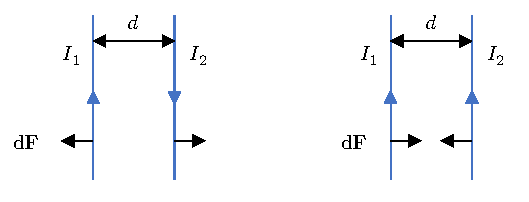
\includegraphics{force_parallel_conductors.pdf}
	\caption{Die Kraft auf parallele, stromdurchflossene Leiter ist anziehend, wenn der Stromfluss in verschiedene Richtungen geht und abstoßend, wenn der Strom in beiden Leiter in der gleichen Richtung fließt. }
	\label{fig:force_parallel_conductors}
\end{figure}

Diese Gleichung beschreibt das historische Biot-Savartsche Gesetz.

Verwendet man Gleichungen \eqref{eq:def_magn_flussdichte} und \eqref{eq:biot_savart}, so erhält man die Kraft zwischen zwei parallelen Leitern mit Abstand $d$ (siehe \Abbref{fig:force_parallel_conductors})
\begin{equation*}
	\frac{\diff\vec F}{\diff z} = \frac{\mu_0}{2\pi} \frac{I_1I_2}d,
\end{equation*}
die orthogonal zum Leiter ist.

Bis zum 20.5.2019 war der Ampère definiert als der Strom, der durch zwei parallele Leiter der Länge $\SI{1}{\m}$ mit $\SI{1}{\m}$ Abstand in gleicher Richtung fließt und eine Anziehungskraft von $\SI{1e-7}{\newton}$ bewirkt.

Heute gilt
\begin{equation*}
	\SI{1}{\ampere}\equiv \frac{\SI{1}{\coulomb}}{\SI{1}{\s}}.
\end{equation*}
Zwischen beliebigen Leiterschleifen $C_{1},C_{2}$ wirkt eine Kraft von
\begin{equation*}
	\vec {F}_{21}=-\vec {F}_{12}=-\frac{\mu _{0}}{4\pi }I_{1}I_{2}\oint _{C_{1}}\oint _{C_{2}}\frac{\vec {r}_{1}-\vec {r}_{2}}{\left| \vec {r}_{1}-\vec {r}_{2}\right| ^{3}}\diff \vec {r}_{1}\cdot \diff \vec {r}_{2}.
\end{equation*}



\section{Grundgleichungen der Magnetostatik}

Um die Grundgleichungen der Magnetostatik herzuleiten, gehen wir zuerst von dem Stromelement $I\diff \vec {r}$ über in die Stromdichte $\vec {j}\left(\vec {r}\right)$ mit $I\diff \vec {r}=\vec {j}\left(\vec {r}\right)\diff^3 \vec {r}$.

Die Kraft auf ein Stromgebiet ist das Integral der Kraftdichte
\begin{equation*}
	\vec {F}=\int \vec f\left(\vec {r}\right)\diffa[3]{\vec{r}}=\int \vec {j}\left(\vec {r}\right)\times \vec {B}\left(\vec {r}\right)\diffa[3]{\vec{r}}.
\end{equation*}
Für eine Punktladung $q$, die sich mit Geschwindigkeit $\vec {v}$ bewegt ($\vec {j}=q\vec {v}\delta \left(\vec {r}-\vec {r}\left(t\right)\right)$) gilt speziell
\begin{equation*}
	\vec F\left(\vec {r}\right)=q\vec {v}\times \vec {B}\left(\vec {r},t\right)
\end{equation*}
bzw. allgemein mit einem zusätzlichen elektrischen Feld
\begin{equation*}
	\vec F\left(\vec {r}\right)=q\left(\vec {v}\times \vec {B}\left(\vec {r},t\right)+\vec {E}\left(\vec {r},t\right)\right).
\end{equation*}
Diese Gesamtkraft ist die sogenannte Lorentzkraft.

Integration des Biot-Savartschen Gesetzes für Leiter führt auf\footnote{vergleichlich mit $\vec {E}(\vec r)=\frac{1}{4\pi \varepsilon _{0}}\int \rho \left(\vec {r}\right)\frac{\vec {r}-\vec {r}'}{\left| \vec {r}-\vec {r}'\right| ^{3}}\diffa[3]{\vec{r}'}$.}
\begin{equation*}
	\vec {B}\left(\vec {r}\right)=\frac{\mu _{0}}{4\pi }\int \vec {j}\left(\vec {r'}\right)\times \frac{\vec {r}-\vec {r}'}{\left| \vec {r}-\vec {r}'\right| ^{3}}\diffa[3]{\vec{r}'}.
\end{equation*}
Wie für das elektrische Feld können wir ein Potential einführen \textendash{} allerdings ist $\vec {B}$ kein Potentialfeld und daher ist das magnetische Potential ein Vektorpotential:
\begin{equation*}
	\vec {B}\left(\vec {r}\right)=\nabla \times \vec {A}\left(\vec {r}\right), \quad\vec {A}\left(\vec {r}\right)=\frac{\mu _{0}}{4\pi }\int \frac{\vec {j}\left(\vec {r}'\right)}{\left| \vec {r}-\vec {r}'\right| }\diffa[3]{\vec{r}'}
\end{equation*}
Die Divergenz von $\vec {B}$ verschwindet, weil stets gilt, dass $\nabla\cdot(\nabla\times \vec A) = 0$.
\begin{formal}
	Das Magnetfeld hat keine Quellen, $\divg \vec {B}=0$.
\end{formal}
In der integralen Formulierung,
\begin{equation*}
	\int _{V}\divg \vec {B}\,\diffa[3]{\vec{r}}=\int _{\partial V}\vec {B}\cdot \diff \vec {f}=0,
\end{equation*}
bedeutet das, dass die magnetischen Feldlinien geschlossen sind. Es gibt folglich keine magnetischen Ladungen, wo die Feldlinien beginnen oder enden.

Für die Rotation der magnetischen Flussdichte gilt
\begin{align}
	\begin{split}
		\label{eq:durchflutungsgesetz_magnetostatik}
		\rot \vec {B}&=\nabla \times \left(\nabla \times \vec {A}\right)=\nabla \left(\nabla \cdot \vec {A}\right)-\nabla ^{2}\vec {A}\\
		&=\frac{\mu _{0}}{4\pi }\nabla \int \vec {j}\left(\vec {r}'\right)\cdot \nabla \frac{1}{\left| \vec {r}-\vec {r}'\right| }\diffa[3]{\vec{r}'}-\frac{\mu _{0}}{4\pi }\int \vec {j}\left(\vec {r}'\right)\nabla ^{2}\frac{1}{\left| \vec {r}-\vec {r}'\right| }\diffa[3]{\vec{r}'}\\
		&=0+\mu _{0}\int \vec {j}\left(\vec {r}'\right)\delta \left(\vec {r}-\vec {r}'\right)\diffa[3]{\vec{r}'}\\&=\mu _{0}\vec {j}\left(\vec {r}\right).
	\end{split}
\end{align}

\begin{formal}
	Elektrische Ströme rufen Wirbel in der magnetischen Flussdichte hervor, $\rot \vec {B}=\mu _{0}\vec {j}\left(\vec {r}\right)$.
\end{formal}
Alternativ kann man sagen, dass die Zirkulation entlang der Oberfläche eines Volumens einem Strom durch das Volumen entspricht,
\begin{equation*}
	\boxed{\int _{\partial F}\vec {B}\cdot \diff \vec {r}=\mu _{0}I.}
\end{equation*}
Diese Gleichung ist als Ampèresches Gesetz bekannt. Mit seiner Nutzung kann man leicht das Magnetfeld von einem homogen stromdurchflossenen, zylindrischen Draht mit Radius $R$ bestimmen, wie in Abbildung \Abbref{fig:cylinder_conductor_with_diagrams} gezeigt. Wähle dazu eine kreisförmige Kurve $C$ mit Radius $r$ um die $z$-Achse herum. Aufgrund der Zylindersymmetrie ist das Magnetfeld nur vom Abstand $r$ der $z$-Achse abhängig und es gilt mit dem Ampèreschen Gesetz
\begin{align*}
	B\left(r\right)\oint _{C}1\diff s & =2\pi rB\left(r\right)=\mu _{0}I\left(r\right) \\
	\equivalence B\left(r\right)      & =\frac{\mu _{0}I\left(r\right)}{2\pi r}.
\end{align*}


\begin{figure}[htb]
	\centering
	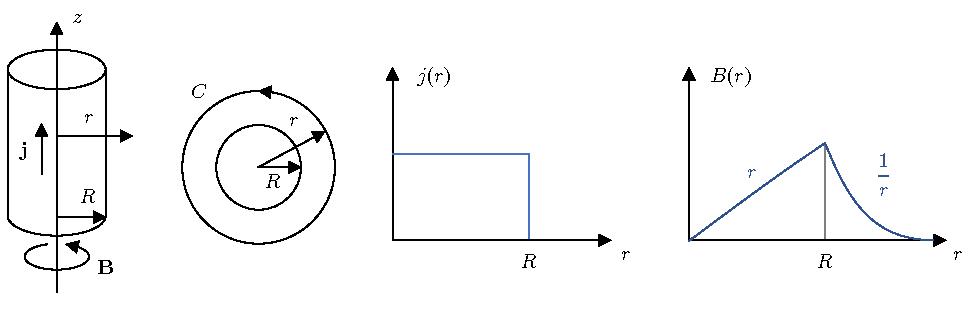
\includegraphics{cylinder_conductor_with_diagrams.pdf}
	\caption{Ein stromdurchflossener, zylindrischer Leiter mit Radius $R$ und Stromdichte $r$ erzeugt ein magnetisches Wirbelfeld. Links: schematische Darstellung, Mitte links: Querschnitt mit gedachter kreisförmiger Kurve $C$ mit Radius $r$ um den Leiter herum, Mitte rechts: Die Stromdichte ist konstant im Leiter und fällt außerhalb auf $0$ ab, rechts: im Leiter steigt der Betrag des Magnetfelds linear mit dem Abstand an und fällt außerhalb ab mit $r^{-1}$.  }
	\label{fig:cylinder_conductor_with_diagrams}
\end{figure}

Der Strom $I\left(r\right)$ enthält nur den Strom, der innerhalb der Kurve $C$ fließt. Innerhalb des zylindrischen Leiters ($r\leq R$) ist die eingeschlossene Fläche gerade $\pi r^{2}$ und damit
\begin{equation*}
	I\left(r\right)=j_{0}\pi r^{2}.
\end{equation*}


\begin{figure}[htb]
	\centering
	\tfigCoil
	\caption{Lange, stromdurchflossenen Spule. }
	\label{fig:long_coil_scheme}
\end{figure}

Außerhalb des Leiters ist $I$ konstant $j_{0}\pi R^{2}$, weil sich der Leiter und damit der Stromfluss nur bis $r=R$ erstreckt. Das Magnetfeld ist also
\begin{align*}
	B\left(r\right)=\frac{\mu _{0}}{2}j_{0}\begin{cases} r,               & r\leq R \\
              \frac{R^{2}}{r}, & r>R
	                                       \end{cases}
\end{align*}
und es ist kreisförmig um die $z$-Achse gerichtet, $\vec {B}\left(r,\varphi \right)=B\left(r\right)\vec {e}_{\varphi }$.

Genauso lässt sich das Feld einer unendlich langen Spule berechnen (\Abbref{fig:long_coil_scheme}):
\begin{align*}
	\oint \vec {B}\cdot \diff \vec {r} & =LB_{0}\overset{!}{=}\mu _{0}NI                   \\
	\implication B_{0}                 & =\mu _{0}\frac{N}{L}I, \vec {B}=B_{0}\vec {e}_{z}
\end{align*}
Zwischen den Windungen hebt sich das magnetische Feld weg.

Wie aus der Gleichung \eqref{eq:durchflutungsgesetz_magnetostatik} hervorgeht, lässt sich für das Vektorpotential $\vec {A}$ wie in der Elektrostatik eine Poissongleichung formulieren,
\begin{equation*}
	\nabla ^{2}\vec {A}=-\mu _{0}\vec {j}
\end{equation*}
und im Potential $\vec {A}\left(\vec {r}\right)$ findet sich wieder eine Greenschen Funktion
\begin{equation*}
	\vec {A}\left(\vec {r}\right)=\int \diffa[3]{\vec{r}'}G\left(\vec {r}-\vec {r}'\right)\vec {j}\left(\vec {r}'\right),\quad G\left(\vec {r}-\vec {r}'\right)=\frac{\mu _{0}}{4\pi }\frac{1}{\left| \vec {r}-\vec {r}'\right| }.
\end{equation*}


\section{Kleine Stromverteilungen: Der magnetische Dipol}

\subsection{Felder kleiner Stromverteilungen}

Wir führen zunächst wieder eine Entwicklung des magnetischen Potentials nach Momenten der Stromverteilung durch:
\begin{equation}
	\label{eq:entwicklung_magn_potential}
	\vec {A}\left(\vec {r}\right)=\frac{\mu _{0}}{4\pi }\int \diffa[3]{\vec{r}'}\frac{\vec {j}\left(\vec {r}'\right)}{\left| \vec {r}-\vec {r}'\right| }\approx \frac{\mu _{0}}{4\pi }\left(\frac{1}{r}\int \diffa[3]{\vec{r}'}\vec {j}\left(\vec {r}'\right)+\frac{\vec {r}}{r^{3}}\cdot \int \diffa[3]{\vec{r}'}\vec {j}\left(\vec {r}'\right)\vec {r}'+\ldots \right)
\end{equation}
Die Auswertung ist allerdings viel komplizierter als für das elektrische Potential und daher beschränken wir uns hier auf die Dipole und vernachlässigen höhere Multipolmomente. Außerdem verwenden wir als Hilfsatz folgende Gleichung, die für beliebige skalare Felder $g$ und $f$ sowie für ein quellenfreies Vektorfeld $\vec {j}$ gilt\footnote{Beweis: Betrachte $\int _{V}\nabla \left(gf\vec {j}\right)\diffa[3]{\vec{r}}$. Einerseits ist dieser Ausdruck mit dem Satz von Gauß gleich $\int _{\partial V}gf\vec {j}\cdot \diff \vec {f}$, was gleich $0$ ist, wenn man das Volumen groß genug wählt, dass auf dem Rand $\vec {j}\left(\vec {r}\right)=\vec {0}$ ist. Außerdem findet man mithilfe der Produktregel, dass $\int _{V}\nabla \left(gf\vec {j}\right)\diffa[3]{\vec{r}}=\int _{V}\vec {j}\cdot \nabla \left(gf\right)\diffa[3]{\vec{r}}+\int _{V}gf\nabla \cdot \vec {j}\diffa[3]{\vec{r}}$, wobei der letzte Term aufgrund der Bedingung $\divg \vec {j}=\vec {0}$ verschwindet, q.e.d.}:
\begin{equation}
	\label{eq:hilfssatz}
	\int \vec {j}\cdot \nabla \left(gf\right)\diffa[3]{\vec{r}}=0.
\end{equation}
Ferner können wir zeigen\footnote{Beweis: Mit der vorigen Formel $\int \vec {j}\cdot \nabla \left(gf\right)\diffa[3]{\vec{r}}=0$ ist mit $g=1$ und $f=x_{i}$ offensichtlicherweise $\int j_{k}\cdot \nabla _{k}x_{i}\diffa[3]{\vec{r}}=\int j_{i}\diffa[3]{\vec{r}}=0$, q.e.d. }, dass
\begin{equation*}
	\int \vec {j}\left(\vec {r}\right)\diffa[3]{\vec{r}}=0,
\end{equation*}
es also keine Strommonopole in $\vec {A}\left(\vec {r}\right)$ gibt. Als letzte Vorbereitung werten wir den zweiten Term in Gleichung \eqref{eq:entwicklung_magn_potential} aus
\begin{equation*}
	\vec {r}\cdot \int \diffa[3]{\vec{r}'}\vec {j}\left(\vec {r}'\right)\vec {r}'=x_{i}\int \diffa[3]{\vec{r}'}x_{i}'j_{k}\left(\vec {r}'\right).
\end{equation*}
Das Produkt $T=x_{i}'j_{k}$ ist ein Tensor zweiter Stufe und lässt sich zerlegen in einen symmetrischen und einen antisymmetrischen Teil, $T_{ik}=\frac{1}{2}\left(T_{ik}+T_{ki}\right)+\frac{1}{2}\left(T_{ik}-T_{ki}\right)$, also
\begin{equation*}
	\vec {r}\cdot \int \diffa[3]{\vec{r}'}\vec {j}\left(\vec {r}'\right)\vec {r}'=x_{i}\int \diffa[3]{\vec{r}'}\left(\frac{1}{2}\left(x_{i}'j_{k}+x_{k}'j_{i}\right)+\frac{1}{2}\left(x_{i}'j_{k}-x_{k}'j_{i}\right)\right).
\end{equation*}
Der erste Summand im Integranden (symmetrischer Teil des Tensors) verschwindet nach dem Hilfssatz \eqref{eq:hilfssatz} mit $g=x_{i}',f=x_{k}'$ und der zweite wird zu
\begin{equation*}
	\frac{1}{2}\int \diffa[3]{\vec{r}'}\left(\left(\vec {r}\cdot \vec {r}'\right)\vec {j}-\left(\vec {r}\cdot \vec {j}\right)\vec {r}'\right)=\frac{1}{2}\int \diffa[3]{\vec{r}'}\left(\vec {r}'\times \vec {j}\right)\times \vec {r}
\end{equation*}
evaluiert.

Nun können wir das magnetische Dipolmoment
\begin{equation*}
	\vec {m}=\frac{1}{2}\int \vec {r}'\times \vec {j}\left(\vec {r}\right)\diffa[3]{\vec{r}'}
\end{equation*}
und das Vektorpotential des magnetischen Dipols
\begin{equation*}
	\vec {A}\left(\vec {r}\right)=\frac{\mu _{0}}{4\pi }\frac{\vec {m}\times \vec {r}}{r^{3}}
\end{equation*}
einführen. Daraus ergibt sich (mit weiteren Umformungen) schließlich das Magnetfeld eines Dipols
\begin{equation*}
	\vec {B}\left(\vec {r}\right)=\rot \vec {A}=-\frac{\mu _{0}}{4\pi }\nabla \frac{\vec {m}\cdot \vec {r}}{r^{3}}=\frac{\mu _{0}}{4\pi }\frac{3\left(\vec {m}\cdot \hat{\vec {r}}\right)\hat{\vec {r}}-\vec {m}}{r^{3}},
\end{equation*}
was wieder völlig analog zum elektrischen Dipol ist.

Wir wollen im Folgenden einmal das Dipolmoment zweier einfacher Geometrien berechnen. Das Dipolmoment einer Stromschleife (\Abbref{fig:magnetic_dipole_field_circle_conductor_ellipsoid}, links) ist einfach (verwende $\vec {j}\diffa[3]{\vec{r}}=I\diff \vec {r}$)
\begin{equation*}
	\vec {m}=\frac{I}{2}\oint \vec {r}\times \diff \vec {r}.
\end{equation*}
Für eine ebene Schleife mit Fläche $F$ und Normalenvektor $\vec {n}$ (\Abbref{fig:magnetic_dipole_field_circle_conductor_ellipsoid}, Mitte) vereinfacht sich dieser Ausdruck zu
\begin{equation*}
	\vec {m}=IF\vec {n}.
\end{equation*}


\begin{figure}[htb]
	\centering
	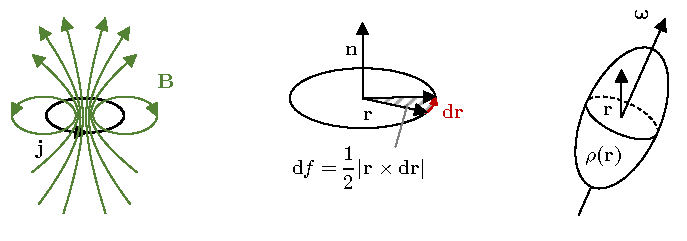
\includegraphics{magnetic_dipole_field_circle_conductor_ellipsoid.pdf}
	\caption{Links: Magnetfeld eines magnetischen Dipols, Mitte: Ein Kreisstrom erzeugt ein magnetisches Dipolmoment, rechts: starrer Körper, der mit $\vec\omega$ rotiert und einer Ladungsverteilung $\rho(\vec r)$ besitzt. }
	\label{fig:magnetic_dipole_field_circle_conductor_ellipsoid}
\end{figure}

Zuletzt betrachten wir einen starren geladenen Körper, der um eine Rotationsachse $\vec {\omega }$ rotiert (\Abbref{fig:magnetic_dipole_field_circle_conductor_ellipsoid}, rechts). Die lokale Geschwindigkeit für eine Ladung in diesem Körper ist $\vec {v}\left(\vec {r}\right)=\vec {\omega }\times \vec {r}$. Die rotierenden Ladungen resultieren in einer Stromdichte $\vec {j}=\rho \vec {v}$, sodass ein Dipolmoment induziert wird:
\begin{equation*}
	\vec {m}=\frac{1}{2}\int d^{3}\vec {r}\,\rho \left(\vec {r}\right)\vec {r}\times \vec {v}.
\end{equation*}
Gleichzeitig besitzt der Körper einen Drehimpuls
\begin{equation*}
	\vec {L}=\int \diffa[3]{\vec{r}}\rho _{m}\left(\vec {r}\right)\vec {r}\times \vec {v}.
\end{equation*}
Trifft man jetzt die Annahme, dass die Verteilungen von Ladung und Masse im Körper gleich sind,
\begin{equation*}
	\frac{\rho \left(\vec {r}\right)}{\rho _{m}\left(\vec {r}\right)}=\frac{q_{\mathrm{ges}}}{m_{\mathrm{ges}}}\equiv \frac{q}{M},
\end{equation*}
dann findet man eine Proportionalität von $\vec {m}$ und $\vec {L}$:
\begin{equation*}
	\vec {m}=\frac{q}{2M}\vec {L}
\end{equation*}
Der Proportionalitätsfaktor $\left| \vec {m}\right| /\left| \vec {L}\right| $ wird als gyromagnetisches Verhältnis bezeichnet. Für den Spin gibt es allerdings eine Abweichung, die aus der Relativitätstheorie hervorgeht und es gilt eigentlich
\begin{equation*}
	\vec {m}=g\frac{q}{2M}\vec {L}
\end{equation*}
mit einem zusätzlichen Landé-Faktor (oder g-Faktor), dessen Wert von der Teilchensorte abhängt. Für Elektronen ist $g\approx 2$, für Protonen $g\approx 2\cdot 2,79$ und für Neutronen $g\approx 2\cdot \left(-1,91\right)$.

Auch die Erde ist ein magnetischer Dipol, der durch Ströme im flüssigen äußeren Erdkern angetrieben wird. Bemerkenswerterweise ist die Dipolachse leicht gegen die Erdachse geneigt und die Polarität dreht sich rund alle 200.000 Jahre um. Der Mechanismus ist allerdings bis heute nicht genau verstanden.

\subsection{Kraft, Drehmoment und Energie}

Die bereits bekannte Kraft auf ein Volumen $V$ mit Stromverteilung $\vec {j}\left(\vec {r}\right)$
\begin{equation*}
	\vec {F}=\int \vec {j}\left(\vec {r}\right)\times \vec {B}\left(\vec {r}\right)\diffa[3]{\vec{r}}
\end{equation*}
lässt sich nach $\vec {B}$ um $\vec {r}=\vec {0}$ Taylor-entwickeln:
\begin{equation*}
	\vec {F}\approx \int \vec {j}\left(\vec {r}\right)\times \left(\vec {B}\left(0\right)+\vec {r}\cdot \nabla \vec {B}\left(0\right)+\ldots \right)\diffa[3]{\vec{r}}=\left(\vec {m}\times \nabla \right)\times \vec {B}\left(0\right)=\nabla \left(\vec {m}\cdot \vec {B}\right)
\end{equation*}
Die potentielle Energie eines Dipols $\vec {m}$ im magnetischen Feld $\vec {B}$ ergibt sich daraus durch Integration
\begin{equation*}
	\vec F=-\nabla U\implication U=-\vec {m}\cdot \vec {B}.
\end{equation*}
Das Minimum wird für $\vec {m} \upupharpoons \vec {B}$ erreicht\footnote{vgl. Funktionsweise von einem Kompass. }. $U$ enthält aber nicht die Energie um den Dipol $\vec {m}$ aufrechtzuerhalten!

Das Drehmoment hat die gleiche Form wie für elektrische Dipole,
\begin{equation*}
	\vec {M}=\vec {m}\times \vec {B}
\end{equation*}
und auch die Wechselwirkungsenergie für einen Dipol im Feld eines zweiten Dipols ist analog
\begin{equation*}
	U=-\frac{\mu _{0}}{4\pi }\frac{3\left(\vec {m}_{1}\cdot \hat{\vec {r}}\right)\left(\vec {m}_{2}\cdot \hat{\vec {r}}\right)-\vec {m}_{1}\cdot \vec {m}_{2}}{r^{3}}.
\end{equation*}



\section{Magnetische Felder in Materie}

Nun behandeln wir magnetische Felder in Materie. Die Vorgehensweise erfolgt analog zu den Kapiteln \ref{sec:mikroskopische_gleichungen_der_elektrostatik} und \ref{sec:Makroskopische_Gleichungen_der_Elektrostatik}. Die freien Ladungen bilden freie Ströme $j_{\mathrm{f}}\left(\vec {r},t\right)$ und gebundene Ladungen fügen jetzt noch gebundene Ströme hinzu $\vec {j}_{\mathrm{b}}\left(\vec {r},t\right)$. Außerdem werden auch magnetische Dipole durch den intrinsischen Spin der Teilchen hinzuaddiert. Die letzten beiden Quellen werden dann gemittelt über eine neue Größe beschrieben: die Magnetisierung.

\subsection{Einführung der Vakuumverschiebungsstromdichte}

In der Magnetostatik haben wir bisher nur
\begin{equation*}
	\nabla \times \vec {B}=\mu _{0}\vec {j},\quad\nabla \cdot \vec {j}=0
\end{equation*}
gehabt. Aber mit der vollständigen Kontinuitätsgleichung
\begin{equation*}
	\frac{\partial }{\partial t}\rho +\nabla \cdot \vec {j}=0
\end{equation*}
brauchen wir eine Verallgemeinerung, wenn $\nabla \cdot \vec {j}\neq 0$:
\begin{equation*}
	\nabla \times \vec {B}=\mu _{0}\vec {j}+\frac{1}{c^{2}}\frac{\partial \vec {E}}{\partial t}=\mu _{0}\left(\vec {j}+\varepsilon _{0}\frac{\partial \vec {E}}{\partial t}\right)
\end{equation*}
Das ist das Ampèresche Gesetz mit der Maxwellschen Verallgemeinerung.

\subsection{Einführung der Magnetisierung}

Wie für die Elektrostatik in Kapitel \ref{sec:mikroskopische_gleichungen_der_elektrostatik} und \ref{sec:Makroskopische_Gleichungen_der_Elektrostatik} beginnen wir, indem wir die mikroskopischen Gleichungen
\begin{equation*}
	\nabla\times \vec {b}=\mu _{0}\left(\vec {j}+\varepsilon _{0}\frac{\partial \vec {e}}{\partial t}\right), \quad\nabla\cdot \vec {b}=0
\end{equation*}
mitteln,
\begin{equation*}
	\vec {B}\left(\vec {r},t\right)=\left\langle \vec {b}\left(\vec {r},t\right)\right\rangle ,\quad \vec {E}\left(\vec {r},t\right)=\left\langle \vec {e}\left(\vec {r},t\right)\right\rangle .
\end{equation*}
Die Stromdichte
\begin{equation*}
	\vec {j}\left(\vec {r},t\right)=\vec {j}_{\mathrm{f}}\left(\vec {r},t\right)+\vec {j}_{\mathrm{b}}\left(\vec {r},t\right)
\end{equation*}
mit "`freien`` Strömen durch einzelne Ladungsträger mit Ladung $q_{i}$ und Geschwindigkeit $v_{i }$
\begin{equation*}
	\vec {j}_{\mathrm{f}}\left(\vec {r},t\right)=\sum _{i\left(f\right)}q_{i}\vec {v}_{i}\delta \left(\vec {r}-\vec {r}_{i}\left(t\right)\right)\implication \vec {j}_{\mathrm{F}}=\left\langle \vec {j}_{\mathrm{f}}\right\rangle .
\end{equation*}
Die gebundenen Ströme werden über alle Moleküle summiert, $\vec {j}_{\mathrm{b}}\left(\vec {r},t\right)=\sum _{n}\vec {j}_{n}\left(\vec {r},t\right)$ mit
\begin{equation*}
	\vec {j}_{n}\left(\vec {r},t\right)=\sum _{i\left(n\right)}q_{i}\vec {v}_{i}\delta \left(\vec {r}-\vec {r}_{i}\right)=\sum _{i\left(n\right)}q_{i}\left(\vec {v}_{n}+\vec {v}_{ni}\right)\delta \left(\vec {r}-\left(\vec {r}_{n}+\vec {r}_{ni}\right)\right)
\end{equation*}
und die Mittelung für das $n$-te Molekül ist (verwende wieder eine Glättungsfunktion $f$)
\begin{equation*}
	\left\langle \vec {j}_{n}\left(\vec {r},t\right)\right\rangle =\sum _{i\left(n\right)}q_{i}\left(\vec {v}_{n}+\vec {v}_{ni}\right)f\left(\vec {r}-\left(\vec {r}_{n}+\vec {r}_{ni}\right)\right).
\end{equation*}
Eine Taylor-Entwicklung um $\vec {r}_{n}$ liefert
\begin{equation*}
	\left\langle \vec {j}_{n}\left(\vec {r},t\right)\right\rangle =\sum _{i\left(n\right)}q_{i}\left(\vec {v}_{n}+\vec {v}_{ni}\right)\left[f\left(\vec {r}-\vec {r}_{n}\right)-\vec {r}_{ni}\cdot \nabla f\left(\vec {r}-\vec {r}_{n}\right)+\ldots \right].
\end{equation*}
Betrachte zunächst die Terme mit $\sum _{i\left(n\right)}q_{i}\vec {v}_{ni}$, die die molekularen Dipolmomente liefern. Der erste Term kann durch ein elektrisches Dipolmoment beschrieben werden:
\begin{equation*}
	\sum _{i\left(n\right)}q_{i}\vec {v}_{ni}=\sum _{i\left(n\right)}q_{i}\frac{\diff \vec {r}_{ni}}{\diff t}=\frac{\diff }{\diff t}\vec {p}_{n}
\end{equation*}
Der zweite Term enthält ein magnetisches Moment (verwende wieder die Tensorzerlegung in einen symmetrischen und einen asymmetrischen Anteil):
\begin{multline*}
	\sum _{i\left(n\right)}q_{i}\left(\vec {r}_{ni}\right)_{\beta }\left(\vec {v}_{ni}\right)_{\alpha }\\
	=\sum _{i\left(n\right)}\frac{1}{2}\left[q_{i}\left(\vec {r}_{ni}\right)_{\beta }\left(\vec {v}_{ni}\right)_{\alpha }-q_{i}\left(\vec {r}_{ni}\right)_{\alpha }\left(\vec {v}_{ni}\right)_{\beta }\right]+\sum _{i\left(n\right)}\frac{1}{2}\left[q_{i}\left(\vec {r}_{ni}\right)_{\beta }\left(\vec {v}_{ni}\right)_{\alpha }+q_{i}\left(\vec {r}_{ni}\right)_{\alpha }\left(\vec {v}_{ni}\right)_{\beta }\right],
\end{multline*}
wobei die Summanden der zweiten Summe verschwinden, weil diese Ströme jeweils auf ein Molekül beschränkt sind ($\nabla\cdot \vec {j}_{\mathrm{b}}=0$). Die erste Summe ist asymmetrisch und lässt sich als Kreuzprodukt schreiben,
\begin{equation*}
	\sum _{i\left(n\right)}q_{i}\left(\vec {r}_{ni}\right)_{\beta }\left(\vec {v}_{ni}\right)_{\alpha }=\frac{1}{2}\varepsilon _{\alpha \beta \gamma }\left(\sum _{i\left(n\right)}q_{i}\left(\vec {r}_{ni}\times \vec {v}_{ni}\right)\right)_{\gamma },
\end{equation*}
sodass sich ein sinnvolles molekulares magnetisches Dipolmoment ergibt,
\begin{equation*}
	\vec {m}_{n}=\frac{1}{2}\sum _{i\left(n\right)}q_{i}\left(\vec {r}_{ni}\times \vec {v}_{ni}\right).
\end{equation*}
Sammle nun alle bisher ausgewerteten Ausdrücke:
\begin{align*}
	\left\langle \left(\vec {j}_{n}\left(\vec {r},t\right)\right)_{\alpha }\right\rangle & =\left(\left(\sum _{i\left(n\right)}q_{i}\left(\vec {v}_{n}\right)_{\alpha }\right)+\frac{\diff }{\diff t}\left(\vec {p}_{n}\right)_{\alpha }\right)f\left(\vec {r}-\vec {r}_{n}\right)                                                                                                                                                                                                                 \\
	                                                                                     & \qquad-\left(\left(\sum _{i\left(n\right)}q_{i}\left(\vec {v}_{n}\right)_{\alpha }\left(\vec {r}_{ni}\right)_{\beta }\right)-\varepsilon _{\alpha \beta \gamma }\left(\vec {m}_{n}\right)_{\gamma }\right)\nabla _{\beta }f\left(\vec {r}-\vec {r}_{n}\right)                                                                                                                                           \\
	                                                                                     & =\left\langle q_{n}\left(\vec {v}_{n}\right)_{\alpha }\delta \left(\vec {r}-\vec {r}_{n}\right)\right\rangle +\frac{\partial }{\partial t}\left\langle \left(\vec {p}_{n}\right)_{\alpha }\delta \left(\vec {r}-\vec {r}_{n}\right)\right\rangle +\varepsilon _{\alpha \beta \gamma }\nabla _{\beta }\left\langle \left(\vec {m}_{n}\right)_{\gamma }\delta \left(\vec {r}-\vec {r}\right)\right\rangle \\
	                                                                                     & \qquad -\nabla _{\beta }\left\langle \left(\vec {v}_{n}\right)_{\alpha }\left(\vec {p}_{n}\right)_{\beta }\delta \left(\vec {r}-\vec {r}_{n}\right)\right\rangle
\end{align*}
Den letzten Term vernachlässigen wir im Folgenden als Term höherer Ordnung (Details sind im Buch von Jackson, Kap. 6.6, zu finden).

Mit diesen Ergebnissen erhalten wir jetzt schlussendlich die gemittelte Stromdichte der gebundenen Ladungen,
\begin{equation*}
	\left\langle \vec {j}_{\mathrm{b}}\left(\vec {r},t\right)\right\rangle =\sum _{n}\left\langle \vec {j}_{n}\left(\vec {r},t\right)\right\rangle =j_{\mathrm{M}}\left(\vec {r},t\right)+\frac{\partial }{\partial t}\vec {P}\left(\vec {r},t\right)+\nabla \times \vec {M}\left(\vec {r},t\right)
\end{equation*}
mit der Stromdichte der gebundenen Ladungen
\begin{equation*}
	\vec {j}_{\mathrm{M}}\left(\vec {r},t\right)=\left\langle \sum _{n}q_{n}\vec {v}_{n}\delta \left(\vec {r}-\vec {r}_{n}\right)\right\rangle ,
\end{equation*}
der makroskopischen Polarisation
\begin{equation*}
	\vec {P}\left(r,t\right)=\left\langle \sum _{n}\vec {p}_{n}\delta \left(\vec {r}-\vec {r}_{n}\right)\right\rangle
\end{equation*}
und der neu eingeführten Magnetisierung (Dichte der magnetischen Dipole)
\begin{equation*}
	\vec {M}\left(\vec {r},t\right)=\left\langle \sum _{n}\vec {m}_{n}\delta \left(\vec {r}-\vec {r}_{n}\right)\right\rangle .
\end{equation*}
Daraus ergibt sich die die gemittelte Stromdichte als Summe der makroskopischen und mikroskopischen Stromdichte,
\begin{equation*}
	\left\langle \vec {j}\left(\vec {r},t\right)\right\rangle =\left\langle \vec {j}_{\mathrm{f}}\left(\vec {r},t\right)\right\rangle +\left\langle \vec {j}_{\mathrm{b}}\left(\vec {r},t\right)\right\rangle =\underset{\vec {j}_{\mathrm{Ma}}}{\underbrace{\vec {j}_{\mathrm{F}}\left(\vec {r},t\right)+\vec {j}_{\mathrm{M}}\left(\vec {r},t\right)}}+\underset{\vec {j}_{\mathrm{Mi}}\left(\vec {r},t\right)}{\underbrace{\frac{\partial }{\partial t}\vec {P}\left(\vec {r},t\right)+\nabla \times \vec {M}\left(\vec {r},t\right)}}
\end{equation*}
und wir können die makroskopischen Feldgleichungen formulieren:
\begin{align*}
	\divg \vec {B} & =0                                                                                                                                                                                            \\
	\rot \vec {B}  & =\mu _{0}\left(\vec {j}_{\mathrm{Ma}}\left(\vec {r},t\right)+\vec {j}_{\mathrm{Mi}}\left(\vec {r},t\right)+\varepsilon _{0}\frac{\partial }{\partial t}\vec {E}\left(\vec {r},t\right)\right) \\
	               & =\mu _{0}\left(\vec {j}_{\mathrm{Ma}}\left(\vec {r},t\right)+\frac{\partial }{\partial t}\vec {D}\left(\vec {r},t\right)+\nabla \times \vec {M}\left(\vec {r},t\right)\right)
\end{align*}
Nun führen wir noch das magnetische Feld $\vec {H}$ ein,
\begin{equation*}
	\vec {H}\left(\vec {r},t\right)=\frac{1}{\mu _{0}}\vec {B}\left(\vec {r},t\right)-M\left(\vec {r},t\right)\equivalence \vec {B}\left(\vec {r},t\right)=\mu _{0}\left(H\left(\vec {r},t\right)+M\left(\vec {r},t\right)\right)
\end{equation*}
Die Magnetisierung $\vec {M}$ wird also wieder in ein Hilfsfeld integriert, was einen einfacheren Ausdruck für die zweite Feldgleichung erlaubt:
\begin{equation*}
	\boxed{\rot \vec {H}=\vec {j}_{\mathrm{Ma}}+\frac{\partial }{\partial t}\vec {D}}
\end{equation*}

\begin{formal}
	Die Wirbel des Magnetfelds $\vec {H}$ sind die makroskopische Stromdichte $\vec {j}_{\mathrm{Ma}}$ und der dielektrische Verschiebungsstrom $\partial _{t}\vec {D}$.
\end{formal}

Das fundamentale magnetische Feld ist die magnetische Flussdichte $\vec {B}$.


\subsection{Materialgesetze und Randbedingungen}

Wir haben bereits gesehen, dass die Felder $\vec {B}$ und $\vec {H}$ über die Magnetisierung in Beziehung stehen:
\begin{equation*}
	\vec {H}=\frac{1}{\mu _{0}}\vec {B}-\vec {M}.
\end{equation*}
Für den Fall, dass die Magnetisierung linear vom Magnetfeld abhängt, führen wir den (linearen) Tensor der magnetischen Suszeptibilität ein,
\begin{equation*}
	M_{i}=\left(\chi _{m}\right)_{ij}H_{j}.
\end{equation*}
Nur wegen der historischen Konvention drücken wir die Magnetisierung als $\vec {M}\left(\vec {H}\right)$ aus und nicht (sinnvollererweise) als $\vec {M}\left(\vec {B}\right)$. Wir schreiben dann also
\begin{equation*}
	\vec {B}=\mu \vec {H}, \mu =\mu _{0}\left(1+\chi _{m}\right)
\end{equation*}
mit dem Tensor der magnetischen Permeabilität $\mu $. Im Allgemeinen ist $\vec {M}\nparallel \vec {H}$.

Sind die Magnetfelder sogar isotrop, kann man einfach schreiben:
\begin{equation*}
	\vec {M}=\chi _{m}\vec {H}, \vec {B}=\mu \vec {H}=\mu _{0}\left(1+\chi _{m}\right)\vec {H}
\end{equation*}
und
\begin{equation*}
	\mu =\mu _{0}\left(1+\chi _{m}\right)\equiv \mu _{0}\mu _{r}.
\end{equation*}
Die dimensionslose Größe $\mu _{r}$ wird als relative Permeabilität bezeichnet.

Bemerkungen:
\begin{itemize}
	\item $\left| \mu _{r}-1\right| $ ist in der Regel in Größenordnungen von $10^{-6}$, also sehr klein.

	\item Bei $\mu _{r}>1$ bzw. $\chi >0$ liegt Paramagnetismus vor, $\vec {M}\parallel \vec {H}$, das heißt, die Ausrichtung der atomaren oder molekularen magnetischen Momente ist entlang $\vec {H}$.

	\item Für $\mu _{r}<1$ bzw. $\chi <0$ spricht man von Diamagnetismus, $\vec {M}\updownharpoons \vec {H}$.
\end{itemize}


Bei Ferromagnetismus gibt es eine permanente Magnetisierung, auch wenn kein Magnetfeld anliegt. Der Zusammenhang zwischen der magnetischen Flussdichte $\vec {B}$ und dem Magnetfeld $\vec {H}$ ist hier nicht linear, wie man an der sogenannten Hysteresekurve (siehe \Abbref{fig:hysterese}) sieht.

\begin{figure}[ht]
	\centering
	\tfighysterese
	\caption{Magnetische Hysterese: An ein zuerst unmagnetisches Material wird ein Feld $H$ angelegt und erhöht. Der Verlauf der magnetischen Flussdichte folgt der Kurve (1) und erreicht schließlich einen Sättigungswert $B_\mathrm{S}$ bei $H_\mathrm{S}$. Wird das Feld auf 0 verringert (Kurve (2)) bleibt eine Magnetisierung zurück (Remanenz). Ein entgegengesetztes Feld von der Stärke der Koerzitivfeldstärke $H_\mathrm{C}$ ist nötig, um die Restmagnetisierung aufzuheben. Jenseits dieser Feldstärke wird die Magnetisierung umgedreht und die Hysteresekurve umgekert durchlaufen. }
	\label{fig:hysterese}
\end{figure}
Zuerst ist das Material unmagnetisch (Punkt im Ursprung). Legt man nun ein Magnetfeld an und erhöht die Feldstärke, erhöht sich der magnetische Fluss im Material entlang der Kurve (1). Dieser wächst aber nicht unbegrenzt, da es schließlich zur Sättigung kommt. Die zugehörige Feldstärke heißt entsprechend Sättigungsfeldstärke $H_{\mathrm{S}}$ und $B_{\mathrm{S}}$ Sättigungswert. Wird nun das Feld wieder verringert, sinkt auch die Flussdichte entlang Kurve (2). Allerdings fällt $B$ nicht bis auf $0$ ab, sondern erreicht den Wert $B_{\mathrm{R}}$, die Remanenzflussdichte. Die Flussdichte fällt erst auf $0$, wenn eine gegengerichtete Koerzitivfeldstärke $H_{\mathrm{C}}$ angelegt wird.

Wir diskutieren nun die Randbedingungen, die im Wesentlichen die gleichen wie in der Elektrostatik sind.

\begin{figure}[ht]
	\centering
	\tfigGrenzflaecheMagnetic
	\caption{Beim Übergang zwischen Medien mit verschiedener Permeabilität ändern sich Magnetfeld und magnetische Flussdichte. Außerdem kann ein Flächenstrom $\vec k$ in der Grenzfläche fließen.
		Die Randbedingungen werden aus Anwendung des Satzes von Gauß auf eine kleine "`Dose`` und des Satzes von Stokes auf eine kleine Schleife, die jeweils einen Teil der Grenzfläche enthalten, hergeleitet. }
	\label{fig:grenzflaeche_magnetic}
\end{figure}

An einer Grenzfläche, wie in \Abbref{fig:grenzflaeche_magnetic} dargestellt, muss die Normalkomponente von $\vec {B}$ stetig sein, da
\begin{equation*}
	\divg \vec {B}=0\quad\xrightarrow[\text{Satz von Gau\ss }]{\text{Dose},\: \Delta  h\rightarrow 0}\quad\hat{\vec {n}}\cdot \left(\vec {B}^{\left(2\right)}-\vec {B}^{\left(1\right)}\right)=0\equivalence B_{\perp }^{\left(1\right)}=B_{\perp }^{\left(2\right)}.
\end{equation*}
Insbesondere ist für ein lineares, isotropes Material auch
\begin{equation*}
	\mu _{1}H_{\perp }^{\left(1\right)}=\mu _{2}H_{\perp }^{\left(2\right)}.
\end{equation*}
Für die Tangentialkomponente von $\vec {H}$ gilt:
\begin{align*}
	\rot \vec {H} & =\vec {j}_{\mathrm{Ma}}+\frac{\partial \vec {D}}{\partial t}\xrightarrow{\text{Schleife}} \int \rot \vec {H}\cdot \diff \vec {f}=\int \vec {H}\cdot \diff \vec {s}=\int \left(\vec {j}_{\mathrm{Ma}}+\frac{\partial \vec {D}}{\partial t}\right)\cdot \hat{\vec {m}}\diff \vec f \\
	              & \xrightarrow{\Delta  h\rightarrow 0}\hat{\vec {t}}\cdot \left(\vec {H}^{\left(2\right)}-\vec {H}^{\left(1\right)}\right)=H_{\parallel }^{\left(2\right)}-H_{\parallel }^{\left(1\right)}=\vec {k}\cdot \hat{\vec {m}}
\end{align*}
mit einem Flächenstrom $\vec {k}$, der noch in der Grenzfläche fließen kann.

Ist das zweite Material sehr leicht magnetisierbar, also $\mu _{2}$ sehr groß gegenüber $\mu _{1}$ und $H^{\left(1\right)}_\parallel\approx 0$, also $\vec {H}^{\left(1\right)}$ orthogonal auf der Grenzfläche (siehe \Abbref{fig:magnetic_refraction}), dann kann das Feld nicht in das zweite Material eindringen ($\vec H^{(2)}\approx 0$) und das letztere verhält sich wie ein elektrischer Leiter, dessen Oberfläche eine Äquipotentialfläche ist.

\begin{figure}[ht]
	\centering
	\tfigMagneticRefraction
	\caption{Treffen die Magnetfeldlinien senkrecht auf eine Grenzfläche zu einem Material mit sehr viel größerer Permeabilität, so dringt das Magnetfeld nicht wesentlich in das zweite Material ein. }
	\label{fig:magnetic_refraction}
\end{figure}

\subsection{Magnetische Skalarpotentiale und ihre Anwendungen}



In der Magnetostatik ist wie wir gesehen haben $\nabla \cdot \vec {B}=0$ und $\nabla \times \vec {H}=\vec {j}$.
\begin{itemize}
	\item Für ein homogenes, lineares Medium ohne Ströme ist $\nabla \times \vec {H}=0$ und wir können $\vec {H}$ als Potentialfeld eines magnetischen Skalarpotentials $\phi _{m}$ schreiben
	      \begin{equation*}
		      \vec {H}=-\nabla \phi _{m}
	      \end{equation*}
	      und mit $\vec {B}=\mu \vec {H}$ und $\nabla \cdot \vec {B}=0$ erhalten wir eine Laplace-Gleichung
	      \begin{equation*}
		      \nabla ^{2}\phi _{m}=0.
	      \end{equation*}
	      Für eine Stromschleife gilt zum Beispiel an einem Punkt $P$
	      \begin{equation*}
		      \phi _{m}\left(P\right)=-\frac{I\Omega  }{4\pi },
	      \end{equation*}
	      wobei $\Omega$ das eingeschlossene Raumwinkelelement ist, siehe \Abbref{fig:ConductorLoopWithRefPoint}.

	      \begin{figure}[htb]
		      \centering
		      \tfigConductorLoopWithRefPoint
		      \caption{Das magnetische Potential einer stromdurchflossenen Leiterschleife mit Fläche $F$ an einem Punkt $P$ ist proportional zu dem Raumwinkelelement, das durch die Projektion der Schleife auf den Punkt $P$ eingeschlossen wird. }
		      \label{fig:ConductorLoopWithRefPoint}
	      \end{figure}
	\item In einem harten Ferromagneten ist $\vec {M}$ vorgegeben und $\vec {j}=0$. Dann ist
	      \begin{equation*}
		      \nabla \cdot \vec {B}=\mu _{0}\nabla \cdot \left(\vec {H}+\vec {M}\right)=0,\quad \vec {H}=-\nabla \phi _{m}
	      \end{equation*}
	      und folglich
	      \begin{equation*}
		      \nabla ^{2}\phi _{m}=-\rho _{m},\quad \rho _{m}=-\nabla \cdot \vec {M}.
	      \end{equation*}
	      In einem Ferromagneten gilt also eine Poisson-Gleichung mit einer effektiven magnetischen Ladungsdichte $\rho _{m}$. Ohne Randflächen ist die Lösung einfach
	      \begin{equation*}
		      \phi _{m}=-\frac{1}{4\pi }\int \frac{\nabla '\cdot \vec {M}\left(\vec {r}'\right)}{\left| \vec {r}-\vec {r}'\right| }\diffa[3]{\vec{r}'}
	      \end{equation*}
	      und mit partieller Integration
	      \begin{equation*}
		      \phi _{m}=-\frac{1}{4\pi }\nabla \cdot \int \frac{\vec {M}\left(\vec {r}'\right)}{\left| \vec {r}-\vec {r}'\right| }\diffa[3]{\vec{r}'}.
	      \end{equation*}
	      Führt man eine Fernfeldentwicklung durch, $1/\left| \vec {r}-\vec {r}'\right| \approx 1/r$ und berücksichtigt nur den ersten Term, so erhält man
	      \begin{equation*}
		      \phi _{m}\left(\vec {r}\right)=-\frac{1}{4\pi }\nabla \left(\frac{1}{r}\right)\cdot \int \vec {M}\left(\vec {r}'\right)\diffa[3]{\vec{r}'}=\frac{1}{4\pi }\frac{\vec {m}\cdot \vec {r}}{r^{3}},
	      \end{equation*}
	      also ein Dipolfeld. Mit Randflächen ist
	      \begin{equation*}
		      \phi _{m}\left(\vec {r}\right)=-\frac{1}{4\pi }\int _{V}\frac{\nabla '\cdot \vec {M}\left(\vec {r}'\right)}{\left| \vec {r}-\vec {r}'\right| }\diffa[3]{\vec{r}'}+\frac{1}{4\pi }\oint _{\partial V}\frac{\vec {n}'\cdot \vec {M}\left(\vec {r}'\right)}{\left| \vec {r}-\vec {r}'\right| }\diff \vec {f}'.
	      \end{equation*}
	      Der Ausdruck $\vec {n}\cdot \vec {M}$ lässt sich als effektive magnetische Flächenladungsdichte $\sigma _{m}$ sehen. Ist die Magnetisierung homogen, dann ist das Potential nur von $\sigma _{m}$ abhängig.
\end{itemize}
Beispiele
\begin{itemize}
	\item Homogen magnetisierte Kugel:
	      \begin{equation*}
		      \phi _{m}\left(\vec {r}\right)=-\frac{1}{4\pi }\vec {M}\cdot \nabla \int _{V_{\mathrm{K}}}\frac{\diffa[3]{\vec{r}'}}{\left| \vec {r}-\vec {r}'\right| }=-\frac{1}{2}\vec {M}\cdot \nabla \int _{0}^{R}\int _{-1}^{1}\frac{r'^{2}\diff r'\diff \cos \vartheta '}{\sqrt{r^{2}+r'^{2}+2rr'\cos \vartheta '}}\diff \vartheta
	      \end{equation*}
	      Im Inneren der Kugel ($r<R$) ist das Ergebnis
	      \begin{equation*}
		      \phi _{m}\left(\vec {r}\right)=\frac{1}{3}\vec {M}\cdot \vec {r}, \quad\vec {H}_{\mathrm{i}}=-\nabla \phi _{m}=-\frac{1}{3}\vec {M},\quad \vec {B}_{\mathrm{i}}=\mu _{0}\left(\vec {H}_{\mathrm{i}}+\vec {M}\right)=\frac{2}{3}\mu _{0}\vec {M},
	      \end{equation*}
	      also $\vec {H}_{\mathrm{i}}\updownharpoons \vec {M}\upupharpoons \vec {B}_{\mathrm{i}}$.

	      Außerhalb der Kugel ist dagegen
	      \begin{equation*}
		      \phi _{m}\left(\vec {r}\right)=\frac{1}{4\pi }\frac{\vec {m}\cdot \vec {r}}{r^{3}},\quad \vec {m}=\frac{4}{3}\pi R^{3}\vec {M}
	      \end{equation*}
	      und
	      \begin{equation*}
		      H_{\mathrm{a}}=\frac{1}{\mu _{0}}\vec {B}_{\mathrm{a}}=-\nabla \phi _{m}
	      \end{equation*}
	      also wieder ein Dipolfeld. Magnetische Flussdichte und Magnetfeld sind in \Abbref{fig:magnetic_field_homogenously_magnetized_ball} dargestellt \textendash{} im Innern der Kugel ist das Magnetfeld entgegen der magnetischen Flussdichte gerichtet. Während $\vec {B}$ ein reines Wirbelfeld ist ($\divg \vec {B}=0$), weist $\vec {H}$ einen Sprung am Kugelrand auf und besitzt damit Quellen $\sigma _{m}=\vec {n}\cdot \vec {M}$.

	      \begin{figure}[htb]
		      \centering
		      \begin{tikzpicture}[
				      scale=.7,
				      mcolor/.style=legreen,
				      pics/graph/.style={background code={
								      \coordinate (O) at (0,0);
								      \coordinate (P) at (1,2);
								      \draw (O) circle [radius=1];
								      \foreach \vzx in {1,-1}{
										      \draw[midarrow] (\vzx*0.5,0.866) ..
										      controls ($1.2*(\vzx*0.5,0.866)$)
										      and (\vzx*1.2, 2.4) .. (\vzx*2.5,3);
										      \draw[midarrow] (\vzx*2.5,-3) ..
										      controls (\vzx*1.2,-2.4)
										      and ($1.2*(\vzx*0.5,-0.866)$) .. (\vzx*0.5,-0.866);
										      \draw[midarrow=.51] (\vzx*0.866,0.5)
										      .. controls +($.8*(\vzx*0.866,0.5)$)
										      and (\vzx*3,1)
										      .. (\vzx*3,0)
										      .. controls (\vzx*3,-1) and ($1.6*(\vzx*0.866,-0.5)$)
										      .. (\vzx*0.866,-0.5) ;
										      \draw[arr] (\vzx*0.866,#1*-0.4) -- (\vzx*0.866,#1*0.4);
										      \draw[arr] (\vzx*0.5,#1*-0.8) -- (\vzx*0.5,#1*0.8);
										      \draw[arr, mcolor] (\vzx*0.7,-0.4) -- +(0,0.8);
										      \draw[arr, mcolor] (\vzx*0.25,-0.4) -- +(0,0.8);
									      }
								      \draw[midarrow=.6] (0,1) -- (0,3.2);
								      \draw[midarrow=.4] (0,-3.2) -- (0,-1);
								      \draw[arr] (0,#1*-.9) -- (0,#1*0.9);
							      }}
			      ]

			      %\pic=1 at (0,0) [transform shape]{graph};
			      %\pic at (7,0) [transform shape]{graph};

			      \draw (0,0) pic[transform shape] {graph=1} node[outer sep=70,above] {$\vec B$-Feld};
			      \draw (7,0) pic[transform shape] {graph=-1} node[outer sep=70,above] {$\vec H$-Feld};
			      \node[mcolor] at (-1.5,0) {$\vec M$};
			      \node[mcolor] at (-1.5+7,0) {$\vec M$};
		      \end{tikzpicture}
		      \caption{Magnetisches Feld und magnetische Flussdichte einer homogen magnetisierten Kugel. Anders als die magnetische Flussdichte $B$ weist das Magnetfeld $H$ einen Sprung (Umpolung) an der Kugeloberfläche auf.  }
		      \label{fig:magnetic_field_homogenously_magnetized_ball}
	      \end{figure}

	\item Magnetisierbare Kugel im äußeren Feld $\vec {B}_{0}$:

	      Mit der Annahme, dass die Magnetisierung $\vec {M}=\left(\mu _{r}-1\right)\vec {H}_{\mathrm{i}}$ linear innerhalb des Kugelvolumens $V_{k}$ ist, erhält man durch Addition der Flussdichte $\vec {B}_{0}$
	      \begin{equation*}
		      \vec {B}_{\mathrm{i}}=\vec {B}_{0}+\frac{2}{3}\mu _{0}\vec {M},\quad \vec {H}_{\mathrm{i}}=\frac{1}{\mu _{0}}\vec {B}_{0}-\frac{1}{3}\vec {M}.
	      \end{equation*}
	      Ähnlich zur Elektrostatik beschreibt $-\vec {M}/3$ ein Entmagnetisierungsfeld. Mittels des linearen Materialgesetzes erhält man schließlich
	      \begin{equation*}
		      H_{\mathrm{i}}=\frac{1}{\mu _{0}}\frac{3}{\mu _{r}+2}\vec {B}_{0}
	      \end{equation*}
	      und
	      \begin{equation*}
		      \vec {M}=\frac{3}{\mu _{0}}\frac{\mu _{r}-1}{\mu _{r}+2}\vec {B}_{0}.
	      \end{equation*}
\end{itemize}

Beim Magnetismus ist alles analog zur Elektrizität AUSSER überall da, wo es genau anders rum ist

\section{Faradaysches Induktionsgesetz}

Bisher haben wir die Elektrostatik und die Magnetostatik getrennt betrachtet. Außerdem haben wir zwar bisher keine Zeitabhängigkeiten berücksichtigt, aber z.B. bereits gesehen, dass zeitabhängige Phänomene eine Rolle spielen, wie zum Beispiel in
\begin{equation*}
	\rot \vec {H}=\vec {j}+\frac{\partial \vec {D}}{\partial t}.
\end{equation*}
Solche sind unter anderem wichtig bei elektromagnetischen Wellen, dem Auf- und Abbau von Feldern etc.

\subsection{Integrale und differentielle Formulierung}

Die Entdeckung des Induktionsgesetzes durch Michael Faraday beruht auf der Beobachtung, dass durch eine Leiterschleife, das einem bewegten magnetischen Feld ausgesetzt ist, ein Strom fließt.

Wir betrachten im Folgenden ein Grundexperiment von Faraday, in dem ein Magnet in der Nähe einer Leiterschleife mit einer Geschwindigkeit $\vec v$ bewegt wird (siehe \Abbref{fig:inductionA}), sodass sich der magnetische Fluss durch die Schleife mit der Zeit ändert.

\begin{figure}
	\centering
	\tfigInductionA
	\caption{Ein Magnetfeld wird in der Nähe einer Leiterschleife $C=\partial F$ bewegt. Der sich ändernde magnetische Fluss bewirkt die Induktion einer Spannung in der Schleife und damit einen Induktionsstrom $I$. }
	\label{fig:inductionA}
\end{figure}

Wir bezeichnen die Leiterschleife als Randkurve $\partial F$ einer Fläche $F$ und führen zwei neue Größen ein: den magnetischen Fluss
\begin{equation*}
	\phi _{B}=\int _{F}\vec {B}\cdot \diff \vec {f}
\end{equation*}
und die elektrische Ringspannung entlang $\partial F$
\begin{equation*}
	Z_{E}=\int _{\partial F}\vec {E}\cdot \diff \vec {r}.
\end{equation*}
Die Ringspannung $Z_{E}$ bewirkt einen Stromfluss in der Schleife. Hiermit und aus den experimentellen Beobachtungen folgte ursprünglich die integrale Formulierung des Induktionsgesetzes
\begin{equation*}
	Z_{E}=-\frac{\diff }{\diff t}\phi _{B}\equivalence \int _{\partial F}\vec {E}\cdot \diff \vec {r}=-\frac{\diff }{\diff t}\int \vec {B}\cdot \diff \vec {f}.
\end{equation*}

\begin{formal}
	Die zeitliche Änderung des magnetischen Flusses durch eine Leiterschleife ruft eine Ringspannung und damit einen Strom hervor.
\end{formal}
Die Bedeutung des negativen Vorzeichens wird mit der Lenzschen Regel erklärt:
\begin{formal}
	Das induzierte elektrische Feld bzw. der induzierte elektrische Strom erzeugt ein Magnetfeld, das der Ursache der magnetischen Flussänderung entgegenwirkt.
\end{formal}
Mit dem Satz von Stokes kann das Induktionsgesetz auch differentiell ausgedrückt werden:
\begin{equation*}
	\rot \vec {E}=-\frac{\partial \vec {B}}{\partial t}
\end{equation*}

\begin{formal}
	Die Wirbel des elektrischen Feldes sind durch die Änderung der magnetischen Flussdichte bestimmt.
\end{formal}


\subsection{Bewegte Leiter}

Bisher haben wir den Leiter festgehalten und das Magnetfeld verändert. Als nächstes soll stattdessen der Leiter bewegt werden, wie in \Abbref{fig:inductionB} dargestellt.

\begin{figure}[ht]
	\centering
	\tfigInductionB
	\caption{Nun wird statt des Magnetfeldes die Leiterschleife mit der Geschwindigkeit $\vec v$ bewegt. }
	\label{fig:inductionB}
\end{figure}

Wir schreiben die treibende Ringspannung wieder als
\begin{equation}
	\label{eq:ringspannung_ruhesystem_leiter}
	Z_{E}=\int _{\partial F}\vec {E}'\cdot \diff \vec {r},
\end{equation}
aber jetzt wird das elektrische Feld im Ruhesystem des Leiters $\vec {E}'$ eingesetzt.

Die Physik soll nach Einsteins Relativitätstheorie in allen Inertialsystemen gleich sein. Eine Beschreibung des Versuchs im Ruhesystem des Leiters muss dasselbe Ergebnis liefern wie im Ruhesystem des Magnetfeldes. Dazu muss die Elektrodynamik invariant unter Lorentz-Transformationen sein. Für kleine Geschwindigkeiten gehen diese Transformationen in Galilei-Transformationen (vernachlässige für diesen Zweck Translationen in Raum und Zeit) $\vec {r}'=\vec {r}-vt$ über. Im Moment werden wir uns auf diese beschränken.

Für den magnetischen Fluss, der jetzt aus dem Integral über eine veränderliche Fläche $F\left(t\right)$ hervorgeht,
\begin{equation*}
	\frac{\diff }{\diff t}\phi _{B}=\frac{\diff }{\diff t}\int _{F\left(t\right)}\vec {B}\left(\vec {r},t\right)\cdot \diff \vec {f},
\end{equation*}
führen wir daher eine Galilei-Transformation durch
\begin{equation*}
	\frac{\diff }{\diff t}\phi _{B}=\frac{\diff }{\diff t}\int _{F}\vec {B}\left(\vec {r}'+\vec {v}t,t\right)\cdot \diff \vec {f}=\int _{F}\frac{\diff }{\diff t}\vec {B}\left(\underset{\vec {r}}{\underbrace{\vec {r}'+\vec {v}t}},t\right)\cdot \diff \vec {f}=\int _{F}\left(\frac{\partial }{\partial t}+\frac{\diff \vec {r}}{\diff t}\cdot \nabla _{\vec {r}}\right)\vec {B}\cdot \diff \vec {f}'.
\end{equation*}
Den zweiten Summanden im Integral schreiben wir um zu
\begin{equation*}
	\frac{\diff \vec {r}}{\diff t}\cdot \nabla _{\vec {r}}\vec {B}=\vec {v}\cdot \nabla _{\vec {r}}\vec {B}=-\nabla \times \left(\vec {v}\times \vec {B}\right)+\vec {v}\left(\nabla \cdot \vec {B}\right)
\end{equation*}
und erhalten
\begin{equation}
	\label{eq:dt_magn_potential}
	\frac{\diff }{\diff t}\phi _{B}=\int _{F}\left(\frac{\partial }{\partial t}-\nabla \times \left(\vec {v}\times \right)\right)\vec {B}\cdot \diff \vec {f}=\int _{F}\frac{\partial }{\partial t}\vec {B}\cdot \diff \vec {f}-\oint _{\partial F}\left(\vec {v}\times \vec {B}\right)\cdot \diff \vec {r}
\end{equation}
Diese Berechnungen wurden im Inertialsystem des Leiters durchgeführt. Nun soll zurück in das Laborsystem (Ruhesystem des Magnetfelds) transformiert werden. Wir wissen bereits, dass
\begin{equation*}
	Z_{e}=-\frac{\diff }{\diff t}\phi _{B}
\end{equation*}
gelten muss. Einsetzen der Gleichungen \eqref{eq:ringspannung_ruhesystem_leiter} und \eqref{eq:dt_magn_potential} führt auf
\begin{equation*}
	\int _{\partial F}\left(\vec {E}'-\vec {v}\times \vec {B}\right)\cdot \diff \vec {r}=-\int _{F}\frac{\partial }{\partial t}\vec {B}\cdot \diff \vec {f}
\end{equation*}
Daraus kann man das elektrische Feld im Laborsystem ablesen:
\begin{equation*}
	\vec {E}=\vec {E}'-\vec {v}\times \vec {B}
\end{equation*}
Dieses Ergebnis ist auch sinnvoll, weil $\rot \vec {E}=\partial _{t}\vec {B}$ erfüllt ist und außerdem die Lorentzkraft auf eine Ladung $q$ im Leiter
\begin{equation*}
	\vec {F}=q\vec {E}'=q\left(\vec {E}+\vec {v}\times \vec {B}\right)
\end{equation*}
ist (im Ruhesystem des Leiters bewegt sich $q$ nicht, im Laborsystem allerdings schon, und zwar mit $\vec {v}$).

\section{Energie des magnetischen Feldes und Induktivität}

\subsection{Energie eines statischen Magnetfeldes}

Die Energie von einem statischen Magnetfeld entspricht genau der Energie, die zum Aufbau des Feldes beim Einschalten des Stroms aufgebracht werden muss. Dabei entstehen aber auch temporäre elektrische Felder, sodass die Induktion berücksichtigt werden muss.

Die Arbeit pro Zeit $\diff _{t}U$, um den Strom $I$ bzw. die Stromdichte $\vec {j}$ aufrecht zu erhalten ist
\begin{equation*}
	\frac{\diff U}{\diff t}=-I\int _{C}\vec {E}\cdot \diff \vec {r}
\end{equation*}
Mit der integralen Formulierung des Induktionsgesetzes gilt also
\begin{equation*}
	\frac{\diff U}{\diff t}=I\frac{\diff }{\diff t}\int \vec {B}\cdot \diff \vec {f}
\end{equation*}
Damit kann man die Energiezunahme, die durch eine Änderung um $\delta \vec {B}$ bewirkt wird, schreiben als
\begin{equation*}
	\delta U=I\int \delta \vec {B}\cdot \diff \vec {f}=I\int \rot \left(\delta \vec {A}\right)\cdot \diff \vec {f}=I\int _{C}\delta \vec {A}\cdot \diff \vec {r}=\int \vec {j}\cdot \delta \vec {A}\diffa[3]{\vec{r}}=\int \left(\nabla \times \vec {H}\right)\cdot \delta \vec {A}\diffa[3]{\vec{r}}.
\end{equation*}
Der Anteil $\partial _{t}\vec {D}$ wird weggelassen, da dieser im Anfangs- und Endzustand gleich $0$ ist. Betrachte zunächst den Integranden
\begin{equation*}
	\left(\nabla \times \vec {H}\right)\cdot \delta \vec {A}=\nabla \cdot \left(\vec {H}\times \delta \vec {A}\right)+\vec {H}\cdot \left(\nabla \times \delta \vec {A}\right).
\end{equation*}
Der erste Summand verschwindet im Integral als Oberflächenterm. Es bleibt\footnote{Zur Erinnerung: In einem Dielektrikum gilt ganz äquivalent $\delta U_{\mathrm{el}}=\int \vec {E}\cdot \delta \vec {D}\diffa[3]{\vec{r}}$. }
\begin{equation*}
	\delta U=\int \vec {H}\cdot \delta \vec {B}\diffa[3]{\vec{r}},
\end{equation*}
bzw. in einem linearen Material
\begin{equation}
	\label{eq:magnetische_energie_linear}
	U=\frac{1}{2}\int \vec {H}\cdot \vec {B}\diffa[3]{\vec{r}}=\frac{1}{2}\int \vec {j}\cdot \vec {A}\diffa[3]{\vec{r}}.
\end{equation}
Alternativ kann man auch die Poisson-Gleichung
\begin{equation*}
	\nabla ^{2}\vec {A}=-\mu \vec {j}\implication \vec {A}=\frac{\mu }{4\pi }\int \frac{\vec {j}\left(\vec {r}'\right)}{\left| \vec {r}-\vec {r}'\right| }\diffa[3]{\vec{r}'}
\end{equation*}
aufstellen und erhält mit Gleichung \eqref{eq:magnetische_energie_linear}
\begin{equation*}
	U = \frac{\mu }{8\pi }\int \diffa[3]{\vec {r}'}\int \diffa[3]{\vec {r}}\frac{\vec {j}\left(\vec {r}\right)\cdot \vec {j}\left(\vec {r}'\right)}{\left| \vec {r}-\vec {r}'\right| }.
\end{equation*}

\subsection{Induktivität}

Mit den Erkenntnissen aus dem letzten Kapitel stellt sich die Frage, wie mehrere Leiterschleifen (wie z.B in \Abbref{fig:TwoInductors} dargestellt) miteinander wechselwirken.

\begin{figure}[ht]
	\centering
	\tfigTwoInductors
	\caption{Mehrere stromdurchflossene Leiterschleifen $C_i$ mit verschiedenen Induktivitäten $L_i$ beinflussen gegenseitig die Energie, die in den Magnetfeldern enthalten ist. }
	\label{fig:TwoInductors}
\end{figure}

Die Feldenergie zweier Leiterschleifen können wir schreiben als
\begin{equation*}
	U=\frac{1}{2}\sum _{i,k}L_{ik}I_{i}I_{k}
\end{equation*}
mit Selbstinduktivität $L_{ii}$ und Gegeninduktivität  $L_{ik},i\neq k$
\begin{align}
	\label{eq:selbstinduktivität}
	L_{ii} & =\frac{\mu }{4\pi }\frac{1}{I_{i}^{2}}\int \int \diffa[3]{\vec{r}}\diffa[3]{\vec{r}'}\frac{\vec {j}_{i}\left(\vec {r}\right)\cdot \vec {j}_{i}\left(\vec {r}'\right)}{\left| \vec {r}-\vec {r}'\right| } \\
	L_{ik} & =L_{ki}=\frac{\mu }{4\pi }\int _{C_{i}}\int _{C_{k}}\frac{\diff \vec {r}_{\mathrm{i}}\cdot \diff \vec {r}_{k}}{\left| \vec {r}-\vec {r}'\right| }
\end{align}
Es lässt sich nun bestimmen, welchen Fluss die Selbstinduktivität erzeugt:
\begin{equation*}
	\phi _{B}=\int \vec {B}\cdot \diff \vec {f}=\int \rot \vec {A}\cdot \diff \vec {f}=\oint _{\partial F}\vec {A}\cdot \diff \vec {r}=\frac{\mu }{4\pi }\oint _{\partial F}\int \frac{\vec {j}\left(\vec {r}'\right)\cdot \diff \vec {r}}{\left| \vec {r}-\vec {r}'\right| }\diffa[3]{\vec{r}'}\equiv LI
\end{equation*}
mit
\begin{equation*}
	L=\frac{\mu }{4\pi }\frac{1}{I}\oint _{\partial F}\int \frac{\vec {j}\left(\vec {r}'\right)\cdot \diff \vec {r}}{\left| \vec {r}-\vec {r}'\right| }\diffa[3]{\vec{r}'}.
\end{equation*}
Mit der Ersetzung $I\diff \vec {r}=\vec {j}\diffa[3]{\vec{r}}$ erhalten wir gerade die Gleichung \eqref{eq:selbstinduktivität}. Die Ringspannung entlang der Leiterschleife ist
\begin{equation*}
	V=\oint \vec {E}\cdot \diff \vec {r}=-\frac{\diff }{\diff t}\phi _{B}=-L\frac{\diff }{\diff t}I.
\end{equation*}
Führen wir eine Verallgemeinerung auf ein System von Leiterschleifen durch, erhalten wir die Ringspannung $V_{i}$ der Schleife $i$
\begin{equation*}
	V_{i}=\oint _{C_{i}}\vec {E}\cdot \diff \vec {r}=-\sum _{k}L_{ik}\frac{\diff }{\diff t}I_{k}.
\end{equation*}
Für einen geraden Draht mit Querschnittsradius $a$ und Länge $h$ (siehe \Abbref{fig:cylindricalConductorAndCoil} links) ist zum Beispiel
\begin{equation*}
	L=\frac{\mu }{2\pi }j\left(\ln \left(\frac{2h}{a}\right)-\frac{3}{4}\right)
\end{equation*}
und für eine unendliche lange Spule mit Querschnittsfläche $A$ und $N$ Windungen pro Länge $h$ (siehe \Abbref{fig:cylindricalConductorAndCoil} rechts)
\begin{equation*}
	L=\mu N^{2}\frac{A}{h},
\end{equation*}
denn $U=HBV/2=\mu H^{2}A/2$ mit $H=NI/h$ liefert
\begin{equation*}
	U=\frac{1}{2}\mu N^{2}I^{2}\frac{A}{h}
\end{equation*}
und
\begin{equation*}
	U=\frac{1}{2}LI^{2}.
\end{equation*}

\begin{figure}[htb]
	\centering
	\tfigcylindricalConductorAndCoil
	\caption{Links: Zylindrisches Drahtstück der Länge $h$ und Radius $a$ in einem Medium mit Permeabilität $\mu$. Rechts: Stück einer (eng gewickelten) Spule der Länge $h$. }
	\label{fig:cylindricalConductorAndCoil}
\end{figure}
% !TEX root = Theo_III.tex


\chapter{Grundgleichungen der Elektrodynamik}

\section{Die Maxwellschen Gleichungen: Zusammenstellung}

Die Maxwellgleichungen bilden die Basis der Elektrodynamik und fast alle Gleichungen zur Beschreibung elektromagnetische Phänomene können aus ihnen hergeleitet werden. Das Ziel ist die Beschreibung der Dynamik von elektrischen und magnetischen \textendash{} den elektromagnetischen \textendash{} Feldern.

Alle Maxwell-Gleichungen wurden in den vorangegangenen Kapiteln bereits in einer oder mehreren Formen behandelt.

Das Gaußsche Gesetz
\begin{equation*}
	\divg \vec {D}=\rho
\end{equation*}
besagt, dass die Quellen des dielektrischen Feldes makroskopische Ladungsdichten sind. Die magnetische Flussdichte hat keine Quellen, es gibt keine magnetischen Monopole und die Feldlinien sind geschlossen,
\begin{equation*}
	\divg \vec {B}=0.
\end{equation*}
Nach dem Faradayschen Induktionsgesetz
\begin{equation*}
	\rot \vec {E}=-\frac{\partial \vec {B}}{\partial t}
\end{equation*}
erzeugen veränderliche Magnetfelder rotierende elektrische Felder. Zuletzt beschreibt das Ampèresche Gesetz (mit Maxwellschem Verschiebungsstrom), dass rotierende Magnetfelder aus Stromdichten und veränderlichen dielektrischen Feldern entstehen,
\begin{equation*}
	\rot \vec {H}=\vec {j}+\frac{\partial \vec {D}}{\partial t}.
\end{equation*}
Diese Gleichungen gelten sowohl im Vakuum als auch in Materie. Dabei ist $\rho \left(\vec {r},t\right)$ die makroskopische Ladungsdichte und $\vec {j}\left(\vec {r},t\right)$ die makroskopische Stromdichte. Diese erfüllen die schon bekannte Kontinuitätsgleichung
\begin{equation*}
	\frac{\partial \rho }{\partial t}+\divg \vec {j}=0.
\end{equation*}
Im Vakuum nehmen die Maxwell-Gleichungen die folgende Form an:
\begin{equation*}
	\divg \vec {E}=\frac{1}{\varepsilon _{0}}\rho ,\quad \rot \vec {E}=-\frac{\partial \vec {B}}{\partial t},\quad \divg \vec {B}=0,\quad \rot \vec {B}=\mu _{0}\vec {j}+\frac{1}{c^{2}}\frac{\partial }{\partial t}\vec {E}
\end{equation*}
Auch die mikroskopischen Maxwellgleichungen haben wir kennengelernt. In Materie wird über stark fluktuierende Felder gemittelt, $\vec {E}=\left\langle \vec {e}\right\rangle $ und $\vec {B}=\left\langle \vec {b}\right\rangle $, sodass für die Ladungs- und Flussdichte gilt:
\begin{align*}
	\left\langle \tilde{\rho }\right\rangle    & =\rho -\nabla \cdot \vec {P}+\partial _{k}\partial _{l}Q_{kl}+\ldots  \\
	\left\langle \tilde{\vec {j}}\right\rangle & =\vec {j}+\frac{\partial }{\partial t}\vec {P}+\nabla \times \vec {M}
\end{align*}
Durch Einführung des dielektrischen Verschiebungsfeldes $\vec {D}$ und des Magnetfeldes $\vec {H}$ als Hilfsfelder erhält man dann die Materialgleichungen
\begin{equation*}
	\vec {D}=\varepsilon _{0}\vec {E}+\vec {P}-\nabla Q, \vec {B}=\mu _{0}\left(\vec {H}+\vec {M}\right)
\end{equation*}
bzw. in linearen Medien einfacher
\begin{alignat*}{4}
	\vec {P} & =\varepsilon _{0}\chi _{e}\vec {E} &  & \implication \vec {D} &  & =\varepsilon \vec {E},\quad &  & \varepsilon =\varepsilon _{0}\left(1+\chi _{e}\right)=\varepsilon _{0}\varepsilon _{r} \\
	\vec {M} & =\chi _{m}\vec {H}                 &  & \implication \vec {B} &  & =\mu \vec {H},\quad         &  & \mu =\mu _{0}\left(1+\chi _{m}\right)=\mu _{0}\mu _{r}.
\end{alignat*}
Die Kraftdichte auf Ladungsdichten und Stromdichten ist
\begin{equation*}
	f\left(\vec {r},t\right)=\rho \vec {E}+\vec {j}\times \vec {B},
\end{equation*}
also gerade die "`Lorentzkraft-Dichte`` als Kontinuumsform der Lorentzkraft.

\section{Elektromagnetische Potentiale}

Eine allgemeine Lösungsstrategie der Maxwellschen Gleichungen liefert die Bestimmung der elektromagnetischen Potentiale. Die Maxwellschen Gleichungen lassen sich als Paare von zwei homogenen Differentialgleichungen,
\begin{equation*}
	\divg \vec {B}=0, \quad\rot \vec {E}+\frac{\partial \vec {B}}{\partial t}=0
\end{equation*}
und zwei inhomogenen Differentialgleichungen,
\begin{equation*}
	\divg \vec {D}=\rho ,\quad \rot \vec {H}-\frac{\partial \vec {D}}{\partial t}=\vec {j}
\end{equation*}
schreiben.

Zuerst werden die homogenen Maxwellgleichungen gelöst. Die zweite Gleichung lässt sich umschreiben zu
\begin{equation*}
	0=\rot \left(\vec {E}+\frac{\partial \vec {A}}{\partial t}\right)\equiv -\rot \left(\nabla \varphi \right).
\end{equation*}
Dabei haben wir ein Vektorpotential $\vec {B}\equiv \nabla \times \vec {A}$ und ein skalares Potential $\vec {E}+\partial _{t}\vec {A}=-\nabla \varphi $ eingeführt. Das magnetische Vektorpotential $\vec {A}$ ist in dieser Form bereits bekannt und das skalare Potential $\varphi $ ist die Verallgemeinerung des elektrischen Potentials auf dynamische Felder.

Die so gewonnenen Gleichungen
\begin{equation}
	\label{eq:equations_for_B_and_E}
	\vec {B}=\rot \vec {A},\quad \vec {E}=-\nabla \varphi -\frac{\partial \vec {A}}{\partial t}
\end{equation}
können jetzt in die inhomogenen Maxwellgleichungen eingesetzt werden, wobei wir uns im Folgenden auf die Gleichungen im Vakuum beschränken. Einsetzen in das Gaußsche Gesetz liefert
\begin{equation}
	\label{eq:dgl_phi_A_rho}
	\nabla ^{2}\varphi +\frac{\partial }{\partial t}\nabla \cdot \vec {A}=-\frac{\rho }{\varepsilon _{0}}
\end{equation}
und aus dem Ampèreschen Gesetz folgt
\begin{equation*}
	\nabla \times \left(\nabla \times \vec {A}\right)=\mu _{0}\vec {j}-\frac{1}{c^{2}}\left(\nabla \frac{\partial \varphi }{\partial t}+\frac{\partial ^{2}\vec {A}}{\partial t^{2}}\right),
\end{equation*}
was man umstellen kann zu
\begin{equation}
	\label{eq:em_wellengleichung}
	\nabla ^{2}\vec {A}=\frac{1}{c^{2}}\frac{\partial ^{2}}{\partial t^{2}}\vec {A}-\nabla \left(\nabla \cdot \vec {A}+\frac{1}{c^{2}}\frac{\partial \varphi }{\partial t}\right)=-\mu _{0}\vec {j}.
\end{equation}
Wir erhalten also insgesamt vier gekoppelte partielle Differentialgleichungen für $\vec {A}$ und $\varphi $ statt acht für $\vec {E}$ und $\vec {B}$. In der Wellengleichung \eqref{eq:em_wellengleichung} können wir zur Bequemlichkeit den D’Alembert-Operator oder auch Wellenoperator
\begin{equation*}
	\Box\equiv\frac{1}{c^{2}}\frac{\partial ^{2}}{\partial t^{2}}-\nabla ^{2}
\end{equation*}
einführen.

In den Gleichungen \eqref{eq:equations_for_B_and_E} sind allerdings die Potentiale $\varphi $ und $\vec {A}$ nicht eindeutig, denn sie können mithilfe einer beliebigen skalaren Eichfunktion $\lambda \left(\vec {r},t\right)$ umgeeicht werden:
\begin{equation}
	\label{eq:umeichung}
	\tilde{\vec {A}}=\vec {A}+\nabla \lambda , \quad\tilde{\varphi }=\varphi -\frac{\partial \lambda }{\partial t}
\end{equation}
Alle auf diese Weise gewonnenen Potentiale $\tilde{\varphi }$ und $\tilde{\vec {A}}$ lassen die physikalischen Felder in \eqref{eq:equations_for_B_and_E} unverändert, was als Eichinvarianz bezeichnet wird. Es wird meist eine spezielle Wahl für die Eichung getroffen.

\subsection{Lorenz-Eichung}

Für die Lorenz-Eichung werden $\vec {A}$ und $\varphi $ so gewählt, dass
\begin{equation}
	\label{eq:lorenzeichung}
	\nabla \cdot \vec {A}+\frac{1}{c^{2}}\frac{\partial \varphi }{\partial t}=0,
\end{equation}
Diese Gleichung ist invariant unter den Lorentz-Transformation der speziellen Relativitätstheorie. Es ergeben sich damit die folgenden inhomogenen Wellengleichungen für $\varphi $ und $\vec {A}$:
\begin{align*}
	\nabla ^{2}\vec {A}-\frac{1}{c^{2}}\frac{\partial ^{2}}{\partial t^{2}}\vec {A} & =-\mu _{0}\vec {j}\equivalence \Box \vec {A}=\mu _{0}\vec {j}                              \\
	\nabla ^{2}\varphi -\frac{1}{c^{2}}\frac{\partial ^{2}}{\partial t^{2}}\varphi  & =-\frac{1}{\varepsilon _{0}}\rho \equivalence \Box \varphi =\frac{1}{\varepsilon _{0}}\rho
\end{align*}
Bemerkenswerterweise sind jetzt die verschiedenen Potentiale entkoppelt. Die Lorenz-Eichung ist immer durchführbar, denn man $\lambda $ nur nach der Differentialgleichung (setze \eqref{eq:umeichung} in \eqref{eq:lorenzeichung} ein)
\begin{equation*}
	\nabla ^{2}\lambda -\frac{1}{c^{2}}\frac{\partial ^{2}}{\partial t^{2}}\lambda =-\left(\nabla \cdot \vec {A}+\frac{1}{c^{2}}\frac{\partial \varphi }{\partial t}\right)
\end{equation*}
zu wählen, was stets möglich ist.


\subsection{Coulomb-Eichung}

Für die Coulomb-Eichung wählt man das magnetische Vektorpotential $\vec {A}$ divergenzfrei, also sodass
\begin{equation*}
	\nabla \cdot \vec {A}=0.
\end{equation*}
Dann gilt mit Gleichung \eqref{eq:dgl_phi_A_rho}
\begin{equation*}
	\nabla ^{2}\varphi =-\frac{1}{\varepsilon _{0}}\rho
\end{equation*}
und $\varphi $ ist gerade das Coulomb-Potential von $\rho $:
\begin{equation*}
	\varphi \left(\vec {r},t\right)=\frac{1}{4\pi \varepsilon _{0}}\int \frac{\rho \left(\vec {r}',t'\right)}{\left| \vec {r}-\vec {r}'\right| }\diffa[3]{\vec{r}'}
\end{equation*}
Aus der Gleichung \eqref{eq:dgl_phi_A_rho} erhält man dann
\begin{equation*}
	\nabla ^{2}\vec {A}-\frac{1}{c^{2}}\frac{\partial ^{2}}{\partial t^{2}}\vec {A}=-\mu _{0}\vec {j}+\frac{1}{c^{2}}\nabla \frac{\partial \varphi }{\partial t}.
\end{equation*}
Auf der rechten Seite erkennen wir den transversalen Anteil der Stromdichte,
\begin{equation*}
	\nabla ^{2}\vec {A}-\frac{1}{c^{2}}\frac{\partial ^{2}}{\partial t^{2}}\vec {A}\equiv\mu _{0}\vec {j}_{t},\quad \vec {j}_{t}=\frac{1}{4\pi }\nabla \times \int \frac{\rot \vec {j}\left(\vec {r}',t'\right)}{\left| \vec {r}-\vec {r}'\right| }\diffa[3]{\vec{r}'}.
\end{equation*}
Man sieht sofort, dass $\divg \vec {j}_{t}=0$, weil $\vec {j}_{t}$ ein reines Wirbelfeld ist.

Wegen $\nabla \cdot \vec {A}=0$ sind die Wellen von $\vec {A}$ transversal, weswegen man auch von der transversalen Eichung oder Strahlungseichung spricht. Das Vektorpotential $\vec {A}$ bestimmt die Wellenausbreitung, während $\varphi $ die statische Lösung beschreibt.

\section{Erhaltungssätze der Elektrodynamik}

\subsection{Erhaltung von Energie: Satz von Poynting}

Wir erinnern uns an die elektromagnetische Kraftdichte, die aus der Lorentzkraft hervorgeht:
\begin{equation*}
	\vec {f}\left(\vec {r},t\right)=\rho \vec {E}+\vec {j}\times \vec {B},\quad \vec {j}=\rho \vec {v}
\end{equation*}
Multiplikation mit der Geschwindigkeit der Ladungsdichte $\vec {v}$ liefert die pro Volumen- und Zeiteinheit geleistete Arbeit des elektrischen Feldes:
\begin{equation*}
	\vec {f}\cdot \vec {v}=\vec {j}\cdot \vec {E}.
\end{equation*}
Sie entspricht genau der mechanischen Arbeit bzw. Jouleschen Wärme. Das magnetische Feld verrichtet keine Arbeit, da $\vec {v}\cdot \left(\vec {j}\times \vec {B}\right)$.

Den Satz von Poynting leiten wir nun her, indem wir das Induktionsgesetz skalar mit dem Magnetfeld $\vec {H}$ multiplizieren und das Durchflutungsgesetz mit dem elektrischen Feld $\vec {E}$ und die beiden Gleichungen subtrahieren:
\begin{equation*}
	\vec {H}\cdot \left(\nabla \times \vec {E}\right)-\vec {E}\cdot \left(\nabla \times \vec {H}\right)=-\vec {j}\cdot \vec {E}-\vec {E}\cdot \frac{\partial \vec {D}}{\partial t}-\vec {H}\cdot \frac{\partial \vec {B}}{\partial t}.
\end{equation*}
Umstellen und Anwenden von $\nabla \cdot \left(\vec {E}\times \vec {H}\right)=\vec {H}\cdot \left(\nabla \times \vec {E}\right)-\vec {E}\cdot \left(\nabla \times \vec {H}\right)$ führt auf die Gleichung
\begin{equation}
	\label{eq:satz_von_poynting}
	\boxed{\vec {E}\cdot \frac{\partial \vec {D}}{\partial t}+\vec {H}\cdot \frac{\partial \vec {B}}{\partial t}+\nabla \cdot \left(\vec {E}\times \vec {H}\right)=-\vec {j}\cdot \vec {E}.}
\end{equation}
Die ersten beiden Terme auf der linken Seite geben die Änderung der elektromagnetischen Feldenergie pro Volumen und Zeiteinheit an. Der Teil $\nabla \cdot \left(\vec {E}\times \vec {H}\right)$ beschreibt den Fluss der elektromagnetischen Feldenergie aus einem Volumen heraus und die rechte Seite ist gerade die mechanische Arbeit bzw. Joulesche Wärme (wie wir gerade gesehen haben), die dem System verloren geht.

Die Größe $\vec {E}\times \vec {H}$ wird als Poynting-Vektor definiert,
\begin{equation*}
	\vec {S}=\vec {E}\times \vec {H}.
\end{equation*}
Er gibt die elektromagnetische Energiestromdichte an und seine Einheit ist dementsprechend Energie pro Fläche und Zeit.

Wir betrachten jetzt zwei Spezialfälle. Im Vakuum und in linearen Materialien ist $\vec {D}=\varepsilon \vec {E}$ und $\vec {B}=\mu \vec {H}$ und wir vernachlässigen Zeitabhängigkeiten von $\varepsilon $ und $\mu $. Mit der elektromagnetischen Feldenergiedichte $u=\left(\vec {E}\cdot \vec {D}+\vec {H}\cdot \vec {B}\right)/2$ lässt sich die Gleichung \eqref{eq:satz_von_poynting} nun umschreiben zu
\begin{equation*}
	\frac{\partial u}{\partial t}+\nabla \cdot \vec {S}=-\vec {j}\cdot \vec {E}
\end{equation*}
bzw. in der integralen Formulierung
\begin{equation*}
	\frac{\diff }{\diff t}\int _{V}u\diffa[3]{\vec{r}}+\int _{\partial V}\vec {S}\cdot \diff \vec {f}=-\int \vec {j}\cdot \vec {E}\diffa[3]{\vec{r}}.
\end{equation*}
Als zweiter Sonderfall sollen linear dispersive Materialien behandelt werden. Die Materialkonstanten $\varepsilon $ und $\mu $ werden als komplexe, frequenzabhängige Konstanten geschrieben,
\begin{equation*}
	\varepsilon \left(\omega \right)=\varepsilon '\left(\omega \right)+i\varepsilon ''\left(\omega \right),\quad \mu \left(\omega \right)=\mu '\left(\omega \right)+i\mu ''\left(\omega \right).
\end{equation*}
Wir betrachten zeitlich periodische (und harmonische) Felder und beschreiben sie durch komplexe Größen:
\begin{align*}
	\vec {E}\left(\vec {r},t\right) & =\vec {E}_{0}\left(\vec {r}\right)e^{-i\omega t},                 & \vec {H}\left(\vec {r},t\right) & =\vec {H}_{0}\left(\vec {r}\right)e^{-i\omega t}         \\
	\vec {D}\left(\vec {r},t\right) & =\varepsilon \left(\omega \right)\vec {E}\left(\vec {r},t\right), & \vec {B}\left(\vec {r},t\right) & =\mu \left(\omega \right)\vec {H}\left(\vec {r},t\right)
\end{align*}
Physikalisch sind natürlich nur die reellen Felder $\vec {E}_{\mathrm{R}}=\mathfrak{R}\left(\vec {E}\right), \vec {H}_{\mathrm{R}}=\mathfrak{R}\left(\vec {H}\right)$ usw. messbar.

Die Änderung der elektromagnetischen Energiedichte lässt sich als Mittelung über eine Periode schreiben:
\begin{align*}
	\dot{u} & =\frac{1}{T}\int _{0}^{T=\frac{2\pi }{\omega }}\left(\vec {E}_{\mathrm{R}}\cdot \frac{\partial \vec {D}_{\mathrm{R}}}{\partial t}+\vec {H}_{\mathrm{R}}\cdot \frac{\partial \vec {B}_{\mathrm{R}}}{\partial t}\right)\diff t                  \\
	        & =\frac{1}{T}\int _{0}^{T=\frac{2\pi }{\omega }}\left(\omega E_{0}^{2}\cos \left(\omega t\right)\left[-\varepsilon '\left(\omega \right)\sin \left(\omega t\right)+\varepsilon ''\left(\omega \right)\cos \left(\omega t\right)\right] \right. \\
	        & \qquad\qquad\qquad \left. +\omega H_{0}^{2}\cos \left(\omega t\right)\left[-\mu '\left(\omega \right)\sin \left(\omega t\right)+\mu ''\left(\omega \right)\cos \left(\omega t\right)\right]\right)\diff t
\end{align*}
Man könnte zuerst denken, dass dieser Ausdruck verschwindet, da die Feldenergie konstant sein sollte. Das Integral der Terme, die den realen Anteil $\varepsilon '$ und $\mu '$ der elektromagnetischen Materialkonstanten enthalten, verschwindet tatsächlich, weil das Produkt $\cos \left(\omega t\right)\sin \left(\omega t\right)$ über eine Periode integriert $0$ ist. Die Terme mit den imaginären Anteilen $\varepsilon ''$ und $\mu ''$ heben sich dagegen nicht auf, weil
\begin{align*}
	\dot{u} & =\frac{\omega }{T}\left(E_{0}^{2}\varepsilon ''\left(\omega \right)+H_{0}^{2}\mu ''\left(\omega \right)\right)\int _{0}^{T=\frac{2\pi }{\omega }}\cos ^{2} \left(\omega t\right)\diff t \\
	        & =\frac{\omega }{2\pi }\left(E_{0}^{2}\varepsilon ''\left(\omega \right)+H_{0}^{2}\mu ''\left(\omega \right)\right)\int _{0}^{2\pi }\cos ^{2} \left(u\right)\diff u                      \\
	        & =\frac{\omega }{2}\left(E_{0}^{2}\varepsilon ''\left(\omega \right)+H_{0}^{2}\mu ''\left(\omega \right)\right).
\end{align*}
Die imaginären Anteile $\varepsilon ''\left(\omega \right)$ und $\mu ''\left(\omega \right)$ der elektromagnetischen Materialkonstanten sind also verantwortlich für die Dissipation der elektromagnetischen Energie.

Wir betrachten jetzt geladene Teilchen und elektromagnetische Felder im Vakuum und führen die "`mechanische`` Energie $u_{\text{mech}}$ ein, bzw. die Energie, die nicht elektromagnetisch ist. Wir können dann wegen
\begin{equation*}
	\frac{\diff u_{\text{mech}}}{\diff t}=\vec {j}\cdot \vec {E}
\end{equation*}
sagen, dass
\begin{equation*}
	\frac{\partial }{\partial t}\left(u_{\text{mech}}+u_{\text{Feld}}\right)+\divg \vec {S}=0.
\end{equation*}
Dies ist die Kontinuitätsgleichung für die Gesamtenergie und beschreibt damit die Energieerhaltung des Systems.

\subsection{Impulserhaltung}

Wenn die "`mechanische`` Energie in elektromagnetische umgewandelt werden kann und umgekehrt, dann ist es auch sinnvoll, analog zum mechanischen Impuls so etwas wie einen Impuls des elektromagnetischen Feldes zu definieren, um eine Kontinuitätsgleichung im Vakuum abzuleiten.

Die zeitliche Änderung des mechanischen Impulses $P_{\text{mech}}$ lässt sich als Integral über die Impulsdichte $p_{\text{mech}}$ beschreiben, dessen zeitliche Änderung gerade der Kraftdichte $f$ entspricht, die durch die Lorentzkraft ausgedrückt werden kann:
\begin{equation*}
	\frac{\diff P_{\text{mech}}}{\diff t}=\frac{\diff }{\diff t}\int p_{\text{mech}}\diffa[3]{\vec{r}}=\int f\left(\vec {r},t\right)\diffa[3]{\vec{r}}=\int \left(\rho \vec {E}+\vec {j}\times \vec {B}\right)\diffa[3]{\vec{r}}
\end{equation*}
Die elektromagnetische Kraftdichte lässt sich mithilfe der Maxwellschen Gleichungen umformen zu
\begin{align*}
	\rho \vec {E}+\vec {j}\times \vec {B} & =\nabla \cdot \vec {D}\vec {E}+\left(\nabla \times \vec {H}-\frac{\partial \vec {D}}{\partial t}\right)\times \vec {B}                                                                                                                                                                                                          \\
	                                      & =\vec {E}\left(\nabla \cdot \vec {D}\right)+\vec {B}\times \frac{\partial \vec {D}}{\partial t}-\vec {B}\times \left(\nabla \times \vec {H}\right)                                                                                                                                                                              \\
	                                      & =\underset{\mathrm{A}}{\underbrace{\vec {E}\left(\nabla \cdot \vec {D}\right)+\left(\nabla \times \vec {E}\right)\times \vec {D}}}-\frac{\partial }{\partial t}\underset{\mathrm{B}}{\underbrace{\left(\vec {D}\times \vec {B}\right)}}-\underset{\mathrm{C}}{\underbrace{\vec {B}\times \left(\nabla \times \vec {H}\right)}}.
\end{align*}
Der Term B beschreibt die neue Impulsdichte des elektromagnetischen Feldes
\begin{equation*}
	p_{\mathrm{em}}=\vec {D}\times \vec {B}=\frac{1}{c^{2}}\vec {E}\times \vec {H}=\frac{1}{c^{2}}\vec {S}.
\end{equation*}
Die $i$-te Komponente vom Term A lässt sich als
\begin{equation*}
	E_{i}\partial _{j}D_{j}-\partial _{i}^{\left(E\right)}\left(E_{j}D_{j}\right)+D_{j}\partial _{j}E_{i}=\partial _{j}\left(E_{i}D_{j}\right)-\frac{1}{2}\partial _{i}\left(E_{j}D_{j}\right)=\partial _{j}\left(E_{i}D_{j}-\frac{1}{2}\delta _{ij}E_{k}D_{k}\right)
\end{equation*}
schreiben (wobei der Differentialoperator $\partial _{i}^{\left(E\right)}$ nur auf Komponente von $E$ wirkt) und die $i$-te Komponente von Teil C als
\begin{equation*}
	\partial _{i}^{\left(H\right)}\left(H_{j}B_{j}\right)+B_{j}\partial _{j}H_{i}+\underset{0}{\underbrace{H_{i}\partial _{j}B_{j}}}=\partial _{j}\left(H_{i}B_{j}-\frac{1}{2}\delta _{ij}H_{k}B_{k}\right).
\end{equation*}
Zusammen können die Terme B und C als Ableitung $\partial _{j}T_{ij}$ eines Tensors $T_{ij}$ geschrieben werden. $T_{ij}$ ist der Maxwellsche Spannungstensor (dessen elektrostatischer Anteil schon aus Kapitel \ref{sec:maxwellscher_spannungstensor} bekannt ist):
\begin{equation*}
	T_{ij}=E_{i}D_{j}+H_{i}B_{j}-\frac{1}{2}\delta _{ij}\left(E_{k}D_{k}+H_{k}B_{k}\right)
\end{equation*}
Er erlaubt eine integrale Beschreibung der Impulsbilanz
\begin{equation*}
	\frac{\diff }{\diff t}\int \left(p_{\text{mech}}+p_{\mathrm{em}}\right)_{i}\diffa[3]{\vec{r}}=\int _{V}\partial _{j}T_{ij}\diffa[3]{\vec{r}}=\int _{\partial V}T_{ij}\diff f_{j}.
\end{equation*}



\end{document}
